\documentclass[conference]{IEEEtran}
\IEEEoverridecommandlockouts
% The preceding line is only needed to identify funding in the first footnote. If that is unneeded, please comment it out.
\usepackage{cite}
\usepackage{amsmath,amssymb,amsfonts}
\usepackage{algorithmic}
\usepackage{graphicx}
\usepackage{textcomp}
\usepackage{xtab}
\usepackage{xcolor}

\pagestyle{plain}
\pagenumbering{arabic}

\def\BibTeX{{\rm B\kern-.05em{\sc i\kern-.025em b}\kern-.08em
    T\kern-.1667em\lower.7ex\hbox{E}\kern-.125emX}}
    
\begin{document}

\title{MC GPT \\
    {\textsuperscript{}- Party Mood Maker \& Play Mini-Games -}
    }

\author{\IEEEauthorblockN{1\textsuperscript{st} Kang JunGyu}
\IEEEauthorblockA{\textit{Dept. of Information Systems } \\
\textit{Hanyang Univ.}\\
Seoul, Republic of Korea \\
jgpk226@gmail.com}
\and
\IEEEauthorblockN{2\textsuperscript{nd} Kim Jihoon}
\IEEEauthorblockA{\textit{Dept. of Information Systems } \\
\textit{Hanyang Univ.}\\
Seoul, Republic of Korea \\
jhkimlego@gmail.com}
\and
\IEEEauthorblockN{3\textsuperscript{rd} Park Jongsu}
\IEEEauthorblockA{\textit{Dept. of Information Systems } \\
\textit{Hanyang Univ.}\\
Seoul, Republic of Korea \\
qwt629@gmail.com}
}

\maketitle

\begin{abstract}
Our team is focusing on providing an application service for making up the mood of parties that are hosted at homes and shared spaces. We plan developing lighting \& appliance control, multiplayer games and space management functions, available to all participants for an entertaining party.\\
We came up with the idea “MC GPT” as we thought of a solution that could release the burden of party hosts and make the party more memorable. Party hosts have many factors to consider such as the lighting of the space, temperature, contents of the party, music and many others. To reduce these tasks focused on the host, our team developed three main functions.\\
First, “MC GPT” has the function to register and control various appliances at any place. For example, lighting devices can be adjusted in color and brightness; other appliances can be adjusted accordingly, such as temperature control of air conditioners. Moreover, we use generative AI to suggest and change the color and brightness of lights according to user inputs.\\
Another function is providing multiplayer mini-games that can be enjoyed with mobile devices of participants. Playing the game involves one game host and other participants. The host can see the questions along with answers of the games, answering orders of participants and moving on to the next games. Participants can view questions of the games and are also provided with an answering button that checks order based on the speed of pressing the button.\\
Finally, space owners can control their spaces by using a unique code generated by the application. These codes can be distributed to other participants which allows them to gain access to all the appliances and games. Importantly, the code can be refreshed which prohibits access from outdated codes.\\
In conclusion, our team hopes to provide appliance control along with a game function that will reduce the tasks required by party hosts, resulting in a more seamless party and help all participants leave with a memorable party experience.
\end{abstract}

\vspace{0.5cm}

\begin{IEEEkeywords}
MC, Manager, Lighting, Appliance, Game
\end{IEEEkeywords}

\section {Role Assignment}

\begin{table}[htbp]
 \begin{tabular}{|p{1cm}|p{1.7cm}|p{5cm}|}
     \hline
     Name & Roles & Task description and etc. \\
     \hline
     Kang JunGyu & Development Manager, Software developer (Back-end) &  
     Development Manager is responsible for managing the overall project. He oversees the functions that are required, the UI/UX configuration, the flawless operation of the prototype, and whether the project proceeds as planned. In addition, he constantly monitors the team member’s progress and whether they are communicating effectively.\\
     \hline
        \end{tabular}
\end{table}
\begin{table}[htbp]
     \begin{tabular}{|p{1cm}|p{1.7cm}|p{5cm}|}
     \hline
     & &
     Software developer (Back-end) is in charge of creating databases, web services, and APIs used by front-end developers. For this position, an understanding of the core database and its features is essential. Every logic as well as integrating with the front-end is developed by him. He uses two tracks of servers, which are the main server and the AI server. The main server interacts with the database, manages user authentication, and handles most server-side logic by Java Spring. The AI Server uses AI codes, open AI, and other libraries for games by Python Flask. He also writes HTTP request codes and WebSocket connection codes on Front-end using React-Native for this project.\\
     \hline
\end{tabular}

 \begin{tabular}{|p{1cm}|p{1.7cm}|p{5cm}|}
     Kim Jihoon & Product Designer, Software developer (AI) & 
     A Product Designer must focus on the usability of a product or service and modify the design of a product to obtain better results. He is responsible for communicating smoothly with other team members and create collaboration.
     A software developer (AI) is responsible for any requirements of the project in terms of data and artificial intelligence. This role selects and refine data into adequate forms in order to make the artificial intelligence model. This role uses machine learning for implementing artificial intelligence to requirements of the software, must run and test model and make a statistical analysis.
     \\
     \hline
     Park Jongsu & Software developer (Front-end), UI/UX Designer & 
     Software Developer(Front-end) is responsible for the creation and implementation of the user interface of web applications. They use technologies like HTML, CSS, and JavaScript to build visually appealing and responsive websites. Their duties involve writing and optimizing code, ensuring compatibility across various devices and browsers, and collaborating with back-end developers. They play a crucial role in optimizing website performance, conducting testing and debugging, and staying updated with the latest front-end development trends and practices.\\
     & & 
     UI/UX Designers focus on the visual and interactive aspects of software applications, designing the user interface and ensuring aesthetics and functionality. They conduct user research to create wireframes and prototypes, collaborate with development teams for accurate implementation, and conduct\\
     \hline
     \end{tabular}
 \end{table}
 
\begin{table}[htbp]
     \begin{tabular}{|p{1cm}|p{1.7cm}|p{5cm}|}
     \hline
     & &
    usability testing. Their role is to create a user-centric, visually appealing, and accessible experience.\\
     \hline
\end{tabular}
\end{table}

\section{Introduction}

    \subsection{Motivation and Term Definition}
        n house parties and Korean ‘MT’s, where many college students and young adults go to have fun these days, the ‘Host’ can  have a hard time controlling the party and provide various recreational content. If the Host was someone other than a human or aided by an app or software, it can ultimately lead to a better party experience. Also everyone could join the party instead of being divided into host and participants, because the host can choose from various functions to lessen the burden of party preparation.\\
    	For a fun MT and house party, not only party games but also setting the party mood is one of the most important things. To do so, our team figured it could be done by providing lighting \& appliance control, mini-games and space control.
        \begin{itemize}
            \item MT : Membership Training in Korea - A party lasts roughly two days and is considered a free-form training session, where students spend time socializing with peers in the same majors or student clubs, often at a remote location.
            \item MC : a Korean phrase used to refer to the official host of the ceremonies, parties, events, or similar performances.
        \end{itemize}

    \subsection{Problem Statements}
        There are a number of issues that arise when hosting parties and games. Running out of game ideas, not enough people to conduct the games, the wrong situation for the party, and more. We will provide a service that will make it simpler for party hosts to manage their party.
        \subsubsection{Why House Parties are Trending}
        
        Home parties have gained popularity in South Korea, especially among the younger generation, for several reasons
        \begin{itemize}
            \item Influence of Social Media: The development of social media platforms made it easier to archive and share special moments. House parties are desired moments worth sharing among many social media users, which resulted in the increase of hosting house parties.
            \item Cost-Effective: House parties are a more budget-friendly option compared to expensive dining or clubbing. Due to recent inflation of the economy, the number of people dining out has decreased significantly. Therefore, sharing simple food and drinks with friends has become a economical option.
            \item Feels Like Home: House parties provide a comfortable and convenient setting to spend time with friends and family, usually following with meaningful interactions and conversations.
            \item Diversity of Activities: House parties offer a range of activities beyond food and drinks, including board games, karaoke, movie nights, dancing, and mini-games.
            \item Cultural Influence: here is a growing interest in Western culture in South Korea, and the concept of house parties from the west may have contributed to their popularity.
        \end{itemize}
        
        \subsubsection{Role of the Party Host}
        As a party host, you need to be in charge of the mood, and you want to keep things interesting and preventing participants from getting bored. Most of all, you want to make sure your guests have a good time.\\
        There are a number of issues that arise when hosting parties and games. Running out of game ideas, not enough people to run the games, the wrong atmosphere for the party and others.\\
        The main role of a house party host is to help guests have a good time and keep the party seamless, but they can't fully enjoy the party with other things to worry about.

    \subsection{Solution}
        We will provide a service that will make it simpler for party hosts to manage their appliances during parties. It will be controlled by using generative AI and providing suggestions.\\
        These days, there are appliances for home parties, but we wanted a way to integrate with smart home systems and devices to make it easy to control multiple devices from one app.\\
        We want to provide  mini-games that require no preparation and is accessible to everyone. We don't want the host to feel stressed about preparing, but rather provide a time for everyone to have fun during the party.

    \subsection{Research on Any Relative Software}
        \subsubsection{Ten-Ten arcade}
            'Ten-Ten' is a multiplayer battle game designed for accessible and enjoyable gaming experiences. The software stands out with its simplicity, allowing users to swiftly create and join game rooms through barcode scanning.\\
            Notable features include real-time multiplayer connectivity, making it ideal for social settings like college events and company orientations. The game offers a diverse range of options, from smartphone-based games to simultaneous multiplayer experiences, catering to varied preferences.\\
            The software's competitive edge lies in its robust ranking and statistics system. Displaying top 100 rankings for each game, it fosters competition and motivates players to challenge themselves. Additionally, the visualization of player activity provides a quick overview of their engagement.\\
            It offers a user-friendly and socially connected multiplayer gaming platform with diverse game options and a compelling ranking system. Its simplicity and versatility make it suitable for various social gatherings and events.\\

        \subsubsection{LG ThinQ}
            LG ThinQ is a comprehensive brand and platform developed by LG Electronics, integrating cutting-edge technologies to enhance the functionality and connectivity of various home appliances and electronic devices. With a focus on artificial intelligence (AI) and smart home solutions, LG ThinQ enables seamless communication and coordination among LG products, with an interconnected ecosystem. Users can control and monitor their devices remotely, leverage AI-driven features for optimized performance, and enjoy a more intuitive and personalized user experience. Whether it's smart TVs, refrigerators, air conditioners, or other appliances, LG ThinQ represents innovation, convenience, and creating a more intelligent and interconnected home environment.
    \section{Requirement Analysis}
    
    \subsection{Logging In}
    Logging in is required for users to have access to functions of the application. Without a login, it is impossible to use any of the functions of the app. If the application is not logged in, users can create their own account or login using an account they have created before. 
    
    \subsection{Creating Account}
    Users can sign up by setting a user id and password of their preference. Signing in requires input  of the given information in the sign up process such as userid, password and name.
    
    \subsection{Space Management}
    “Space” refers to any type of place where parties can be held and added to the software. Space management mainly focuses on space creation and space connection. Space creation means making a new space so that it can be used to link with electronics and made available for others to join. Space connection means gaining access to spaces via the code provided by owners. Each space has a unique code which can be shared with others and is required to access the functions provided. The code can be generated by creating a space in the application and request code generation on the settings tab. Also, Space management is separated into 2 types of classes;owners and users.\\ \\
    Space owner: Can generate random authentication codes for individual spaces. Also, it is possible to refresh the code which terminates the validity of the code for previous users, forcing them to lose access of the space.\\ \\
    Space user: A space user can gain access to spaces with the code provided by the owner. By having the code, the user also has access to the lighting and appliances pre-registered by the Space owner.

    \subsection{Status Dashboard}
    Users can view the status of the space upon logging into the software. It is the first page that a user will encounter upon connecting to a space. The dashboard acts as the main page of the application. It includes the name of the space, a simple announcement bar, data on space temperature and air quality. The name of the space is provided by owners, space temperature and air quality information comes from data on the related appliance. Also, it contains a music player where all users with access can add desired songs to a shared playlist. It is connected to whatever music output device that is present at the space, which means controlling the music player will have an effect on the sound of the space for everyone. 

    \subsection{Lighting Control}
    Provides controlling any hardware with lighting function. Users can change the brightness, color and effects of the lights using the software. It is not just for lighting devices but also for any kind of appliance that has a lighting function such as a NUGU candle or LG Mood-Up refrigerator Also, users can input any type of situation desired in natural language and the lighting will automatically change accordingly using AI. The input can be made by a input box using a keyboard or by requesting it in speech to an AI speaker. To help users that cannot make a decision for which lighting to use, there will be some preset requests available to execute.

    \subsection{Appliance Control}
    Provides control of any appliances that are synced with the software, such as changing the space temperature using an air conditioner, checking remaining beer amount on Homebrew,  setting the power of a air purifier. It will be functioning as a shared setting, which means any user can adjust the appliance. This will help make the environment of the party adequete for party instantly. Also, space owners can lock certain appliances, which results in prohibiting users from access to the locked appliance. Locking option can be activated by toggling a lock icon inside the appliance settings

    \subsection{Party Games}
    Users can play games from a list of games provided. There are 2 types of users in the process of the game, operator and participant. \\
    
    Game operator: Page consist of the answer of the game, a list to check the answering order, buttons for moving on to the next game and quitting the game for everyone\\
    
    Game participant: Page consist of the game question and a push button for confirming the answering order, which is in first-come-first-served basis.\\
    
    Currently there will be 3 games that will be serviced, however it is possible to include various games since the format is shared. The list of serviced games are as following.\\

    \begin{itemize}
        \item Image game: An AI model merges the face of two celebrities, the participants are asked to guess the celebrities based on the merged image.
        \item Landmark guessing game: The game receives the coordinates of famous landmarks around the world from OpenAI API. The data is sent to Google map API for a street view photo of the coordinate. Participants are required to guess the landmark from the street view photo.
        \item Gather up: Game operator first inputs the number of participants. NUGU speaker plays any music for about 10 seconds, stop the music and tell how many people to gather up. Then, participants gather up according to the given number and participants who could not gather up are eliminated. The process will be entirely conducted by the NUGU speaker, and the given number will be calculated by a pre-set algorithm
    \end{itemize}
    
\section{Development Environment}
    \subsection{Choice of Software}
        \subsubsection{Estimated Cost}
            \begin{itemize}
                \item AWS EC2 \& S3: About 3 USD per month
            \end{itemize}
    \begin{table}[htbp]
        \caption{Development Language and Environment}
        \centering
        \begin{tabular}{| p{1.2cm}|p{6.8cm} |} 
             \hline
             Tools and Language & Description and Reason for Selection \\ [0.5ex]
             \hline
             Spring & Spring is a comprehensive and widely adopted framework for building Java-based enterprise applications. It provides a range of tools and libraries that simplify the development of large-scale, robust, and highly maintainable applications. The Spring framework addresses various aspects of application development, aspect-oriented programming, and transaction management. Spring facilitates the development of enterprise-class applications and microservices by promoting best practices and modularity. It's an essential tool for Java developers looking to streamline application development and improve code quality.\\
            &
            The reasons for choosing Spring framework over others is first, has a characteristic that the developer does not depend on particular libraries or container stacks. Also, in the process of database synchronization(when working on a scale of status change), it is fairly simple to annotate transactions. Most of all, it is very popular that has the biggest community and a very stable framework. \\
             \hline
             React
             
             Native & React Native is an open-source UI software framework created by Meta Platform, Inc. It is used to develop applications for Android, Android TV, iOS, macOS, tvOS, Web, Windows and UWP by enabling developers to use the React framework along with native platform capabilities. It is also being used to develop virtual reality applications at Oculus. One of the biggest feature of React Native is being able to create native UI for Android and iOS using JavaScript, and create high-quality UI faster than using HTML.
             React Native communicates with Native Thread over native bridges, optimizing performance unlike web apps. Using a method of communicating with the native without using this web is called a Hybrid App, and there are Xamarin, Native Script, and flutter.
             In this project, we chose React Native for developing mobile applications in the frontend development environment because it offers a wealth of resources, and it supports native development environments for both Android and iOS, making it a superior choice over other mobile app programming frameworks.\\
             \hline
             Python & Python is a high-level, versatile, and dynamically-typed programming language known for its simplicity and readability. It has a vast standard library and a thriving ecosystem of third-party packages and frameworks, which makes it suitable for a wide range of applications, including web development, data analysis, machine learning. Python's syntax is clear and expressive, making it an ideal language for both beginners and experienced developers. It supports multiple programming paradigms, including procedural, object-oriented, and functional programming. Python has gained significant popularity in recent years for data science and machine learning thanks to libraries like NumPy, pandas, scikit-learn, and TensorFlow. It is also used in web development with frameworks like Flask. Python's simplicity, versatility, and large community make it one of the most popular programming languages in the world.\\
             \hline
        \end{tabular}
    \end{table}
    
\begin{table}[htbp]
    \centering
        \begin{tabular}{| p{1.2cm}|p{6.8cm} |}
             \hline
             PostgreSQL &  PostgreSQL, often referred to as "Postgres," is a powerful open-source relational database management system (RDBMS). It's known for its advanced features and extensibility, making it a popular choice for both small and large-scale applications. PostgreSQL offers robust support for structured data, ACID compliance, and features like indexing, full-text search, and geospatial capabilities. It is highly extensible and allows developers to create custom functions and data types. With a strong focus on data integrity and security, PostgreSQL is widely used in a variety of industries, including web applications, data warehousing, and geographic information systems (GIS). \\ [1ex]
             \hline
        \end{tabular}
    \end{table}
    
    \begin{table}[htbp]
        \caption{Development Language and Environment}
        \centering
        \begin{xtabular}{|p{2cm}|p{4cm}|}
        \hline
        Name & Develop Environment\\
        \hline
        Kang Jungyu & 
        macOS Sonoma 14.0 \hfill \break Spring, Flask\\
        \hline
        Kim Jihoon & 
        macOS Sonoma 14.0 \hfill \break Pytorch, TeXLive\\
        \hline
        Park Jongsu & 
        macOS Sonoma 14.0 \hfill \break React-Native, Figma\\
        \hline
        \end{xtabular}
    \end{table}

    \newpage
    \subsection{Software in Use}
    
        \begin{figure}[htbp]
        \centerline{
\includegraphics[width=5cm]{Images/logo/github.png}}
        \label{fig}
        \caption{Logo of GitHub}
        \end{figure}
        \subsubsection{GitHub}
        GitHub is an indispensable platform in the world of software development. It serves as a web-based hub that plays a pivotal role in version control and team collaboration, allowing developers to efficiently manage their source code. It is particularly known for its Git-based repository hosting, which enables developers to store, manage, and monitor changes in their codebase. GitHub provides a range of features designed to streamline the development process, including code repositories for version control, pull requests for peer review, and issue tracking for tracking and managing project tasks and bugs. Developers can work on different branches of a project simultaneously and merge their changes seamlessly. This fosters collaboration among team members and ensures the integrity of the codebase. GitHub has become an essential tool for distributed software development, enabling remote teams to work together seamlessly.\\
        
        \begin{figure}[htbp]
        \centerline{
\includegraphics[width = 4.5cm]{Images/logo/intellij.png}}
        \label{fig}
        \caption{Logo of IntelliJ IDEA}
        \end{figure}
        \subsubsection{IntelliJ IDEA}
        IntelliJ IDEA is a powerful integrated development environment (IDE) that is specifically designed for Java developers. It offers a plethora of tools and features to streamline Java software development. The IDE provides intelligent code completion, allowing developers to write code faster and with fewer errors. It also offers extensive code analysis, which can detect potential issues and suggest improvements in real-time. The IDE supports popular Java frameworks, libraries, and build tools, making it a valuable tool for Java developers. Its user-friendly interface and extensive plugin support further enhance the development experience.\\
    
        \begin{figure}[htbp]
        \centerline{
\includegraphics[width=5cm]{Images/logo/vsc.png}}
        \label{fig}
        \caption{Logo of Visual Studio Code}
        \end{figure}
        \subsubsection{Visual Studio Code}
        Visual Studio Code, commonly referred to as VS Code, is a highly versatile and extensible code editor developed by Microsoft. It has gained immense popularity in the software development community, not only for its support of multiple programming languages but also for its role in mobile app development, including React Native. VS Code offers syntax highlighting, code navigation, and debugging tools that are indispensable for React Native development. Developers can write and debug code efficiently and take advantage of a vast library of extensions to tailor the editor to their specific needs. It is a lightweight but powerful tool for web and mobile app development, offering a seamless and customizable development experience. It was chosen and being used to compile React-Native codes for our project.\\
    
    
        \begin{figure}[htbp]
        \centerline{
\includegraphics[width=4.5cm]{Images/logo/xcode.png}}
        \label{fig}
        \caption{Logo of Xcode}
        \end{figure}
        \subsubsection{Xcode}
         Xcode is Apple's official integrated development environment (IDE) specifically designed for macOS and iOS app development. It serves as a comprehensive toolset for developing applications for Apple platforms, including iOS, macOS, watchOS, and tvOS. Xcode includes a code editor with features like code completion, code analysis, and integrated debugging, making it an indispensable tool for writing code for Apple's ecosystem. It also provides a graphical interface builder that simplifies the design of user interfaces for iOS apps. Furthermore, Xcode streamlines the app development process by offering tools for testing, profiling, and app distribution through the App Store. It is a complete package for building, testing, and deploying high-quality applications on Apple devices.\\
    
        \begin{figure}[htbp]
        \centerline{
\includegraphics[width=7cm]{Images/logo/pycharm.png}}
        \label{fig}
        \caption{Logo of PyCharm}
        \end{figure}
        \subsubsection{PyCharm}
        PyCharm, also developed by JetBrains, is an indispensable integrated development environment (IDE) for Python developers. It offers a set of features designed to streamline Python software development. PyCharm's code editor includes intelligent code completion, which suggests code snippets and identifies potential errors as you type. This feature significantly improves code quality and development speed. The IDE also supports various Python frameworks and libraries, making it easier to work with popular technologies like Django and Flask. It also simplifies virtual environment management, which is crucial for Python project isolation and package management.\\
        
        \begin{figure}[htbp]
        \centerline{
\includegraphics[width=4.5cm]{Images/logo/jupyter.png}}
        \label{fig}
        \caption{Logo of Jupyter Notebook}
        \end{figure}
        \subsubsection{Jupyter Notebook}
        Jupyter Notebook is an open-source web application that allows users to create and share documents that contain live code, equations, visualizations, and narrative text. It's widely used for data analysis, scientific computing, and machine learning. Jupyter Notebooks support various programming languages, including Python.. These notebooks are composed of cells that can contain code, text, or visual outputs, making it a valuable tool for creating reproducible research and data-driven documents. It provides an interactive and user-friendly environment for data exploration, analysis, and sharing. Jupyter Notebook is a preferred among data scientists, researchers, and educators for its flexibility and interactivity.\\

        \begin{figure}[htbp]
        \centerline{
\includegraphics[width=5cm]{Images/logo/expo.png}}
        \label{fig}
        \caption{Logo of Expo}
        \end{figure}
        \subsubsection{Expo}
        Expo is a set of tools and services that simplifies the development of React Native applications. It provides a variety of pre-built components and libraries, making it easier for developers to create mobile apps without the need for extensive native code development. Expo also offers a development client that allows developers to preview their applications on physical devices without the need for complex setup. It's a valuable tool for rapidly prototyping and developing mobile applications and can be especially useful for developers looking for a simplified and accelerated development process.\\

        \begin{figure}[htbp]
        \centerline{
\includegraphics[width=7cm]{Images/logo/aws.png}}
        \label{fig}
        \caption{Logo of AWS EC2}
        \end{figure}
        \subsubsection{AWS EC2}
        AWS EC2, part of Amazon Web Services, is a scalable and flexible cloud computing platform that provides virtual servers known as instances. These instances can be customized to run various operating systems and applications, making it a cornerstone for cloud-based software development. Developers can launch, manage, and scale virtual machines based on their needs. AWS EC2 offers various instance types optimized for different workloads, including compute, memory, and storage-optimized instances, enabling developers to choose the right infrastructure for their applications. It plays a critical role in building and deploying web applications, backend services, and other software solutions in the cloud.\\
        
        \begin{figure}[htbp]
        \centerline{
\includegraphics[width=6cm]{Images/logo/awss3.png}}
        \label{fig}
        \caption{Logo of AWS S3}
        \end{figure}
        \subsubsection{AWS S3}
        AWS S3, part of the Amazon Web Services suite, is a highly scalable object storage service. It provides developers with a secure and durable solution for storing and retrieving data in the cloud. Using S3, developers can create storage buckets to organize and manage their data, whether it be for static website hosting, data archiving, or backup. AWS S3 offers features such as versioning, access control, and seamless integration with other AWS services. Its reliability and scalability make it a fundamental component for data storage in various cloud-based applications and services.\\

        \begin{figure}[htbp]
        \centerline{
\includegraphics[width=4.5cm]{Images/logo/openai.png}}
        \label{fig}
        \caption{Logo of OpenAI}
        \end{figure}
        \subsubsection{OpenAI API}
        OpenAI API is a powerful artificial intelligence service provided by OpenAI. It allows developers to integrate natural language processing and generation capabilities into their applications. With OpenAI API, developers can build applications that understand, generate, and interact with human-like text. It's designed to handle a variety of language tasks, such as text completion, language translation, and conversation generation. OpenAI API empowers developers to create intelligent and context-aware applications, enhancing the overall user experience with advanced language understanding.\\

        \begin{figure}[htbp]
        \centerline{
\includegraphics[width=4.5cm]{Images/logo/forge.png}}
        \label{fig}
        \caption{Logo of Miniforge}
        \end{figure}
        \subsubsection{Miniforge}
        Miniforge is a distribution of the popular Conda package manager, optimized for minimalism and efficiency. Conda is used for managing packages and environments in data science and scientific computing. Miniforge is designed for users who want to create lightweight, customizable environments for specific tasks. It allows you to create isolated and reproducible environments for different Python projects, making it easier to manage dependencies and packages. Miniforge is especially valuable for data scientists and researchers who need to create custom Python environments for their work and prefer a minimalistic approach to package management. It was used in our project to create virtual environments for machine learning codes.\\

        \begin{figure}[htbp]
        \centerline{
\includegraphics[width=5.5cm]{Images/logo/datagrip.png}}
        \label{fig}
        \caption{Logo of DataGrip}
        \end{figure}
        \subsubsection{DataGrip}
        DataGrip, developed by JetBrains, is a specialized database management tool essential in software development. It supports multiple database systems, making it an all-in-one solution for related tasks. DataGrip offers a wide range of features, including SQL code development, schema visualization, and data exploration, simplifying database management through a unified interface for various engines. It enables developers to write and execute SQL queries, analyze data structures, and optimize performance. Intelligent code completion, real-time analysis, and database navigation features expedite development and management.\\

        \begin{figure}[htbp]
        \centerline{
\includegraphics[width=5.5cm]{Images/logo/postman.png}}
        \label{fig}
        \caption{Logo of Postman}
        \end{figure}
        \subsubsection{Postman}
        Postman is a versatile tool for simplifying API testing and working in software development. It serves as an API development and testing platform, enabling developers to create, send, and monitor HTTP requests. Acting as an API client, Postman allows developers to interact with API endpoints, test functionality, and ensure correct operation. It supports automation by enabling the creation of request collections and automated testing. Postman offers a user-friendly interface for request building and organization, facilitating collaboration between developers and testers.\\

        \begin{figure}[htbp]
        \centerline{
\includegraphics[width=5.5cm]{Images/logo/colab.png}}
        \label{fig}
        \caption{Logo of Google Colab}
        \end{figure}
        \subsubsection{Google Colab}
        Google Colab is a cloud-based platform for machine learning and data analysis that provides free access to a virtual machine with GPUs. It runs in a web browser and offers a Jupyter Notebook interface, making it a convenient tool for writing and executing code for data science and machine learning projects. Google Colab allows users to run Python code, perform data analysis, and train machine learning models using GPU acceleration, which can significantly speed up computations. It's a powerful resource for data scientists and machine learning engineers who need a cost-effective way to perform compute-intensive tasks without investing in local hardware.\\

        \begin{figure}[htbp]
        \centerline{
\includegraphics[width=4.5cm]{Images/logo/nugu.png}}
        \label{fig}
        \caption{Logo of Nugu Developers}
        \end{figure}
        \subsubsection{NUGU Playbuilder}
        NUGU Playbuilder is a development platform provided by NUGU, an AI assistant developed by SK Telecom. It is specifically designed for creating voice-activated and conversational AI applications and services. NUGU Playbuilder simplifies the process of building voice interfaces and chatbots, allowing developers to design and implement natural language interactions. This platform provides tools for creating voice scripts, defining dialogue flows, and integrating with various data sources and services, making it a valuable asset for developers looking to create AI-powered applications and services.\\

        \begin{figure}[htbp]
        \centerline{
\includegraphics[width=5cm]{Images/logo/figma.png}}
        \label{fig}
        \caption{Logo of Figma}
        \end{figure}
        \subsubsection{Figma}
        Figma is a popular web-based design and prototyping tool known for its collaborative and user-friendly features. It empowers designers to create user interfaces, prototypes, and design components with real-time collaboration, ideal for cross-functional teams. It simplifies sharing design assets with developers, providing a platform for design handoff. Developers can inspect design specs, export assets, and collaborate with designers in real-time. Figma's flexibility and cloud-based approach facilitate seamless communication between designers and developers throughout a project's design and development phases.\\

        \begin{figure}[htbp]
        \centerline{
\includegraphics[width=5cm]{Images/logo/notion.png}}
        \label{fig}
        \caption{Logo of Notion}
        \end{figure}
        \subsubsection{Notion}
        Notion is a versatile workspace that caters to the diverse needs of software development teams. It combines note-taking, task management, knowledge sharing, and collaborative documentation. Notion offers a flexible and customizable platform for organizing information, managing projects, and sharing knowledge. Teams can structure their work using pages, databases, and boards, with support for various data types like text, tables, files, and multimedia content. Notion excels in project management, enabling task lists, reminders, and collaboration on project boards. Notion's seamless collaboration features concurrent work on the same page, making it a valuable tool for collaboration.\\

        \begin{figure}[htbp]
        \centerline{
\includegraphics[width=5.5cm]{Images/logo/slack.png}}
        \label{fig}
        \caption{Logo of Slack}
        \end{figure}
        \subsubsection{Slack}
        Slack is a highly popular communication platform designed to enhance collaboration and communication within software development teams. It offers real-time messaging, file sharing, and integration with various software tools. Slack simplifies team communication by providing chat channels for different topics or teams, direct messaging, and file sharing capabilities. Developers can create channels dedicated to specific projects or discussions, making it easy to organize and find conversations. One of Slack's key strengths is its extensive library of integrations with third-party tools. It allows teams to connect other software tools, like GitHub and Google Drive, directly to their Slack workspace, streamlining workflows and enhancing productivity. Slack also supports notification customization, ensuring that team members receive updates and alerts relevant to their roles and responsibilities. It plays a crucial role in fostering efficient communication, project discussion, and workflow optimization within software development teams.\\

        \begin{figure}[htbp]
        \centerline{
\includegraphics[width=5cm]{Images/logo/overleaf.png}}
        \label{fig}
        \caption{Logo of Overleaf}
        \end{figure}
        \subsubsection{Overleaf}
        Overleaf is a web-based platform designed for collaborative scientific writing and document preparation, especially for LaTeX documents. It simplifies the process of creating complex documents with mathematical equations, tables, and references. Overleaf offers real-time collaboration features, enabling multiple authors to work on the same document simultaneously. It provides a rich text editor with LaTeX support and a compilation engine, allowing authors to see real-time previews of their documents. It's a valuable tool for researchers and academics who need to create and collaborate on scholarly documents and reports. Also, it has a feature where it can be synced with GitHub and committed to a repository.\\

        \begin{figure}[htbp]
        \centerline{
\includegraphics[width=4.5cm]{Images/logo/texlive.png}}
        \label{fig}
        \caption{Logo of TeXLive}
        \end{figure}
        \subsubsection{TeXLive}
        TeX Live is a comprehensive distribution of the TeX typesetting system, which is widely used for document preparation in fields such as scientific and technical publishing, academia, and literature. It is cross-platform, supporting Windows, macOS, and Linux, and provides a vast collection of packages and fonts to address a wide range of document types and formats. TeX Live is renowned for its high-quality typesetting and is often used to create documents with complex layouts, mathematical notation, and bibliographies. It is the go-to choice for authors and researchers who require precise control over the visual appearance of their documents.\\
        
\section{Specification}
    \subsection{Loading Page}
        When a application communicates with servers, a delay is inevitable in the process. During the delay, it might show just a blank screen to users. To prevent users from getting a blank page, a loading screen will appear instead. This applies to all functions that require server communication including login, register, space creation, space connection and etc. \\
        This loading page UI is made by ‘skeleton’ from React Native. While receiving data from the server, components without received data shows that it is loading. In other words, while server is processing and receiving data after a http request has been made by the client. It can make a seamless and user friendly UI by using the loading screen.
    \subsection{Login Page}
        \begin{figure}[htbp]
            \centerline{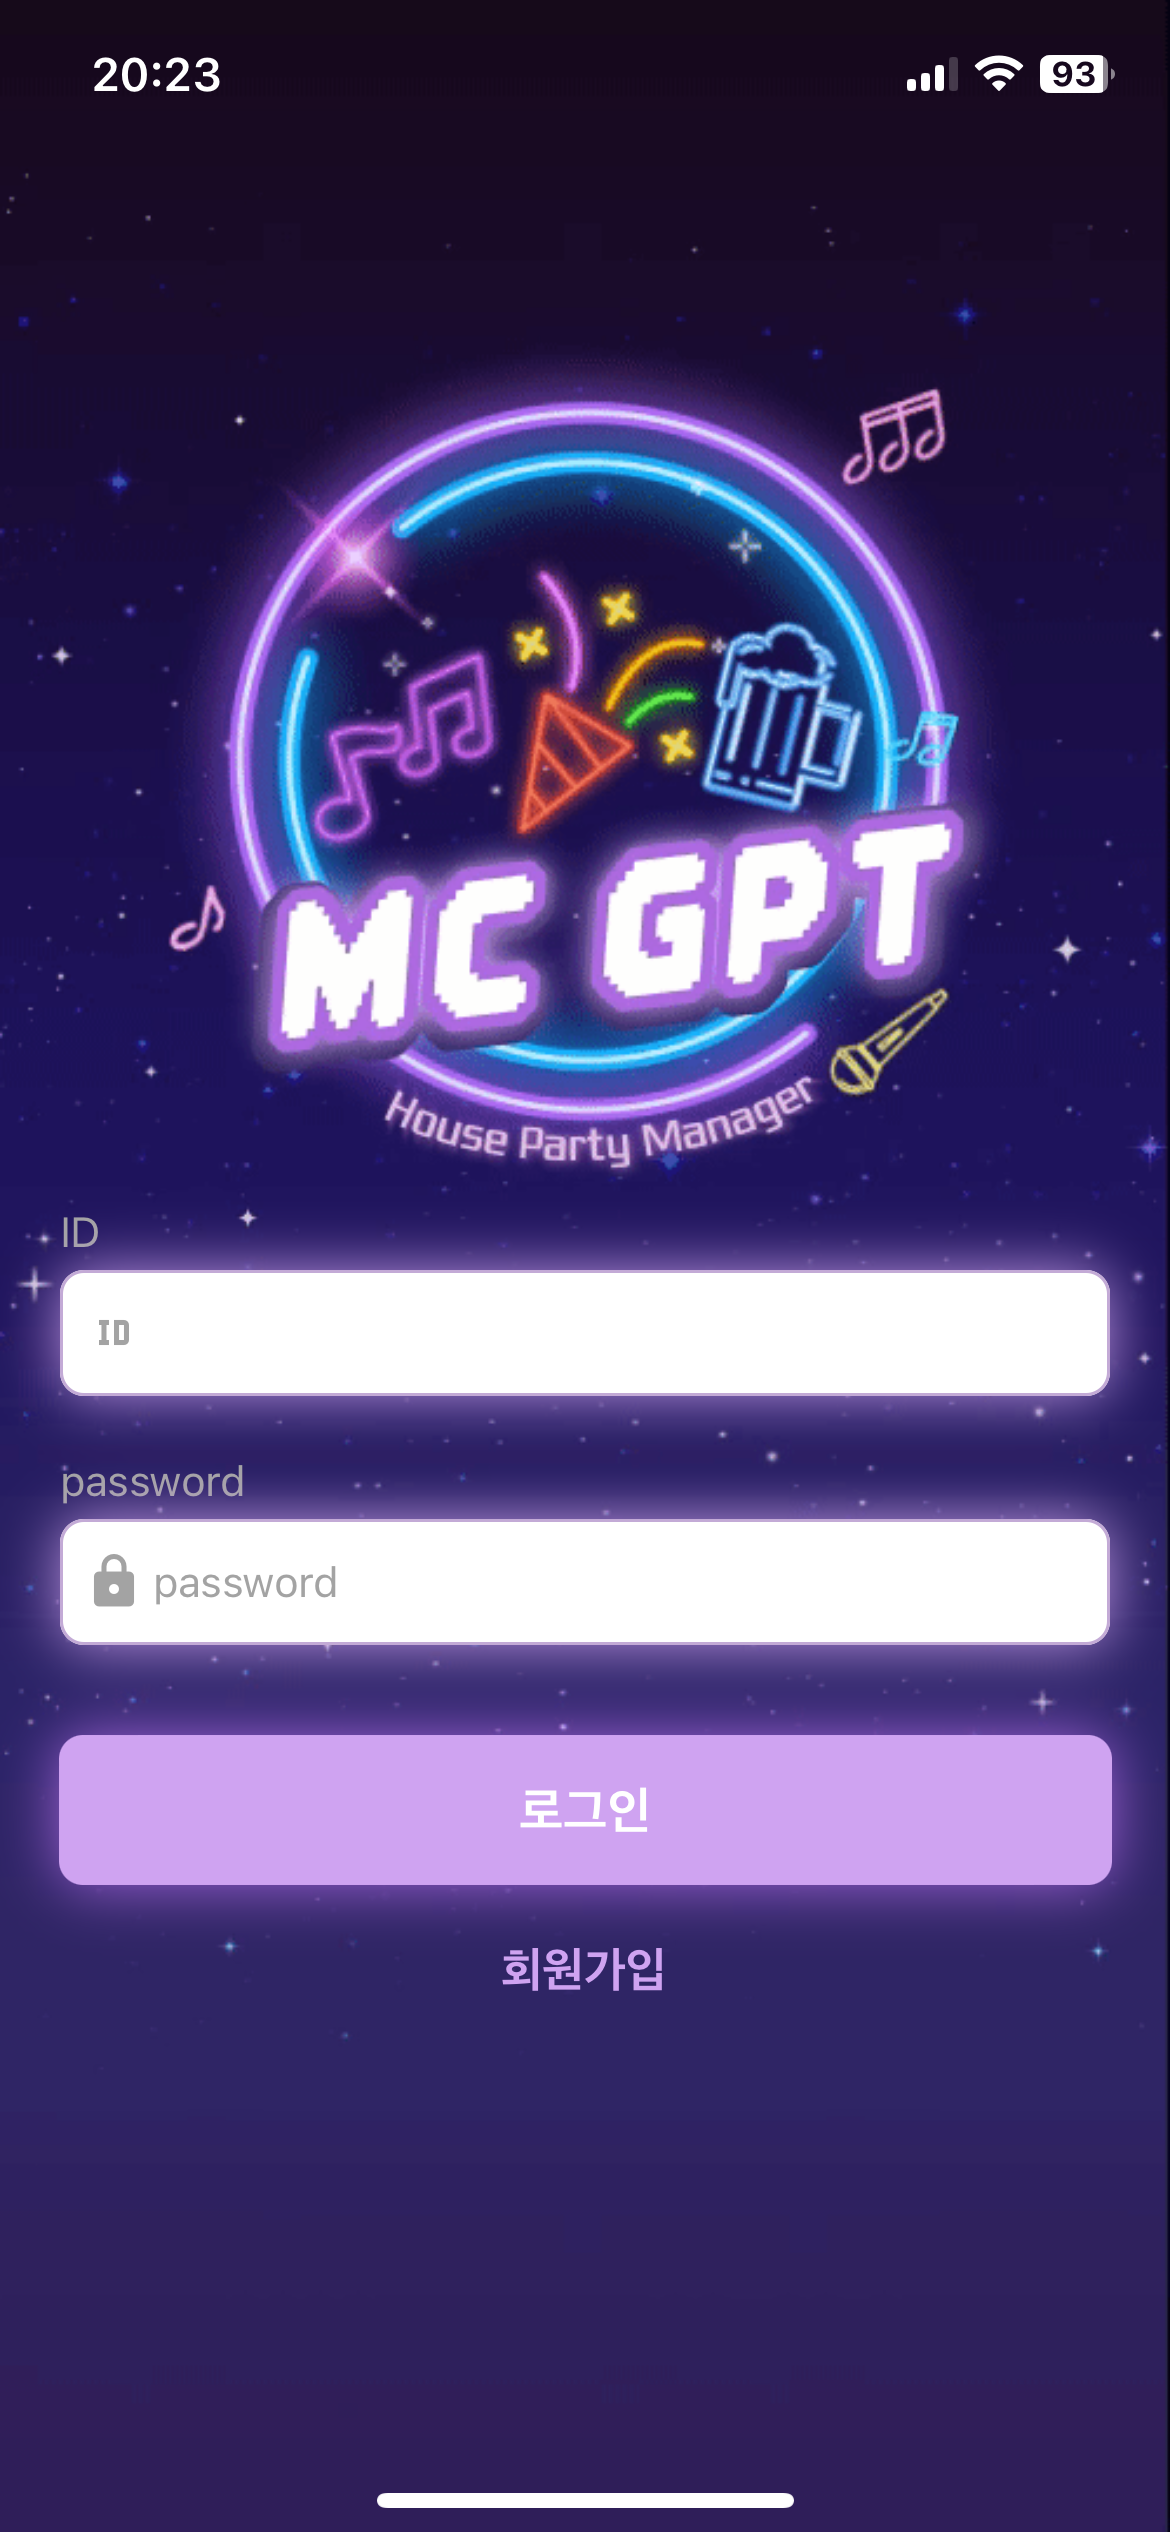
\includegraphics[width=3cm]{Images/screen/login/LOGIN_EMPTY.PNG}}
            \label{fig}
            \caption{Login Page}
        \end{figure}
        Logging in is required for users to have access to functions of the application. Without a login, it is impossible to use any of the functions of the app. If the application is not logged in, users can create their own account or login using an account they have created before. \\
        In a back-end point of view, The client receives an ID and password from the user and sends a request to the server when a button is pressed. On the server, it checks if there is ‘Member’ data in the DB and, if it exists, returns a security token known as JWT. The token expires after a certain time for security reasons and needs to be refreshed.  The client stores the JWT and includes it in the header of every request sent. \\
        In a front-end point of view, When a user clicks on the ID input field or the password input field, the input field's border is emphasized, and a keyboard appears. The screen moves up when the keyboard appears to ensure that it does not cover the screen.  If the user enters their ID and then presses the next button on the keyboard, it automatically transits to the password input field. The password displayed on the screen is encrypted while it is being entered.  Both the ID and password must be entered for the login button to become active. When the login button is pressed, it changes to a loading screen while the login process is executed on the server. After the login process is completed, the screen transitions to a page with a list of spaces. If the login fails, an Alert message is displayed, and the user remains on the login screen.
    \subsection{Register Page}
        \begin{figure}[htbp]
            \centerline{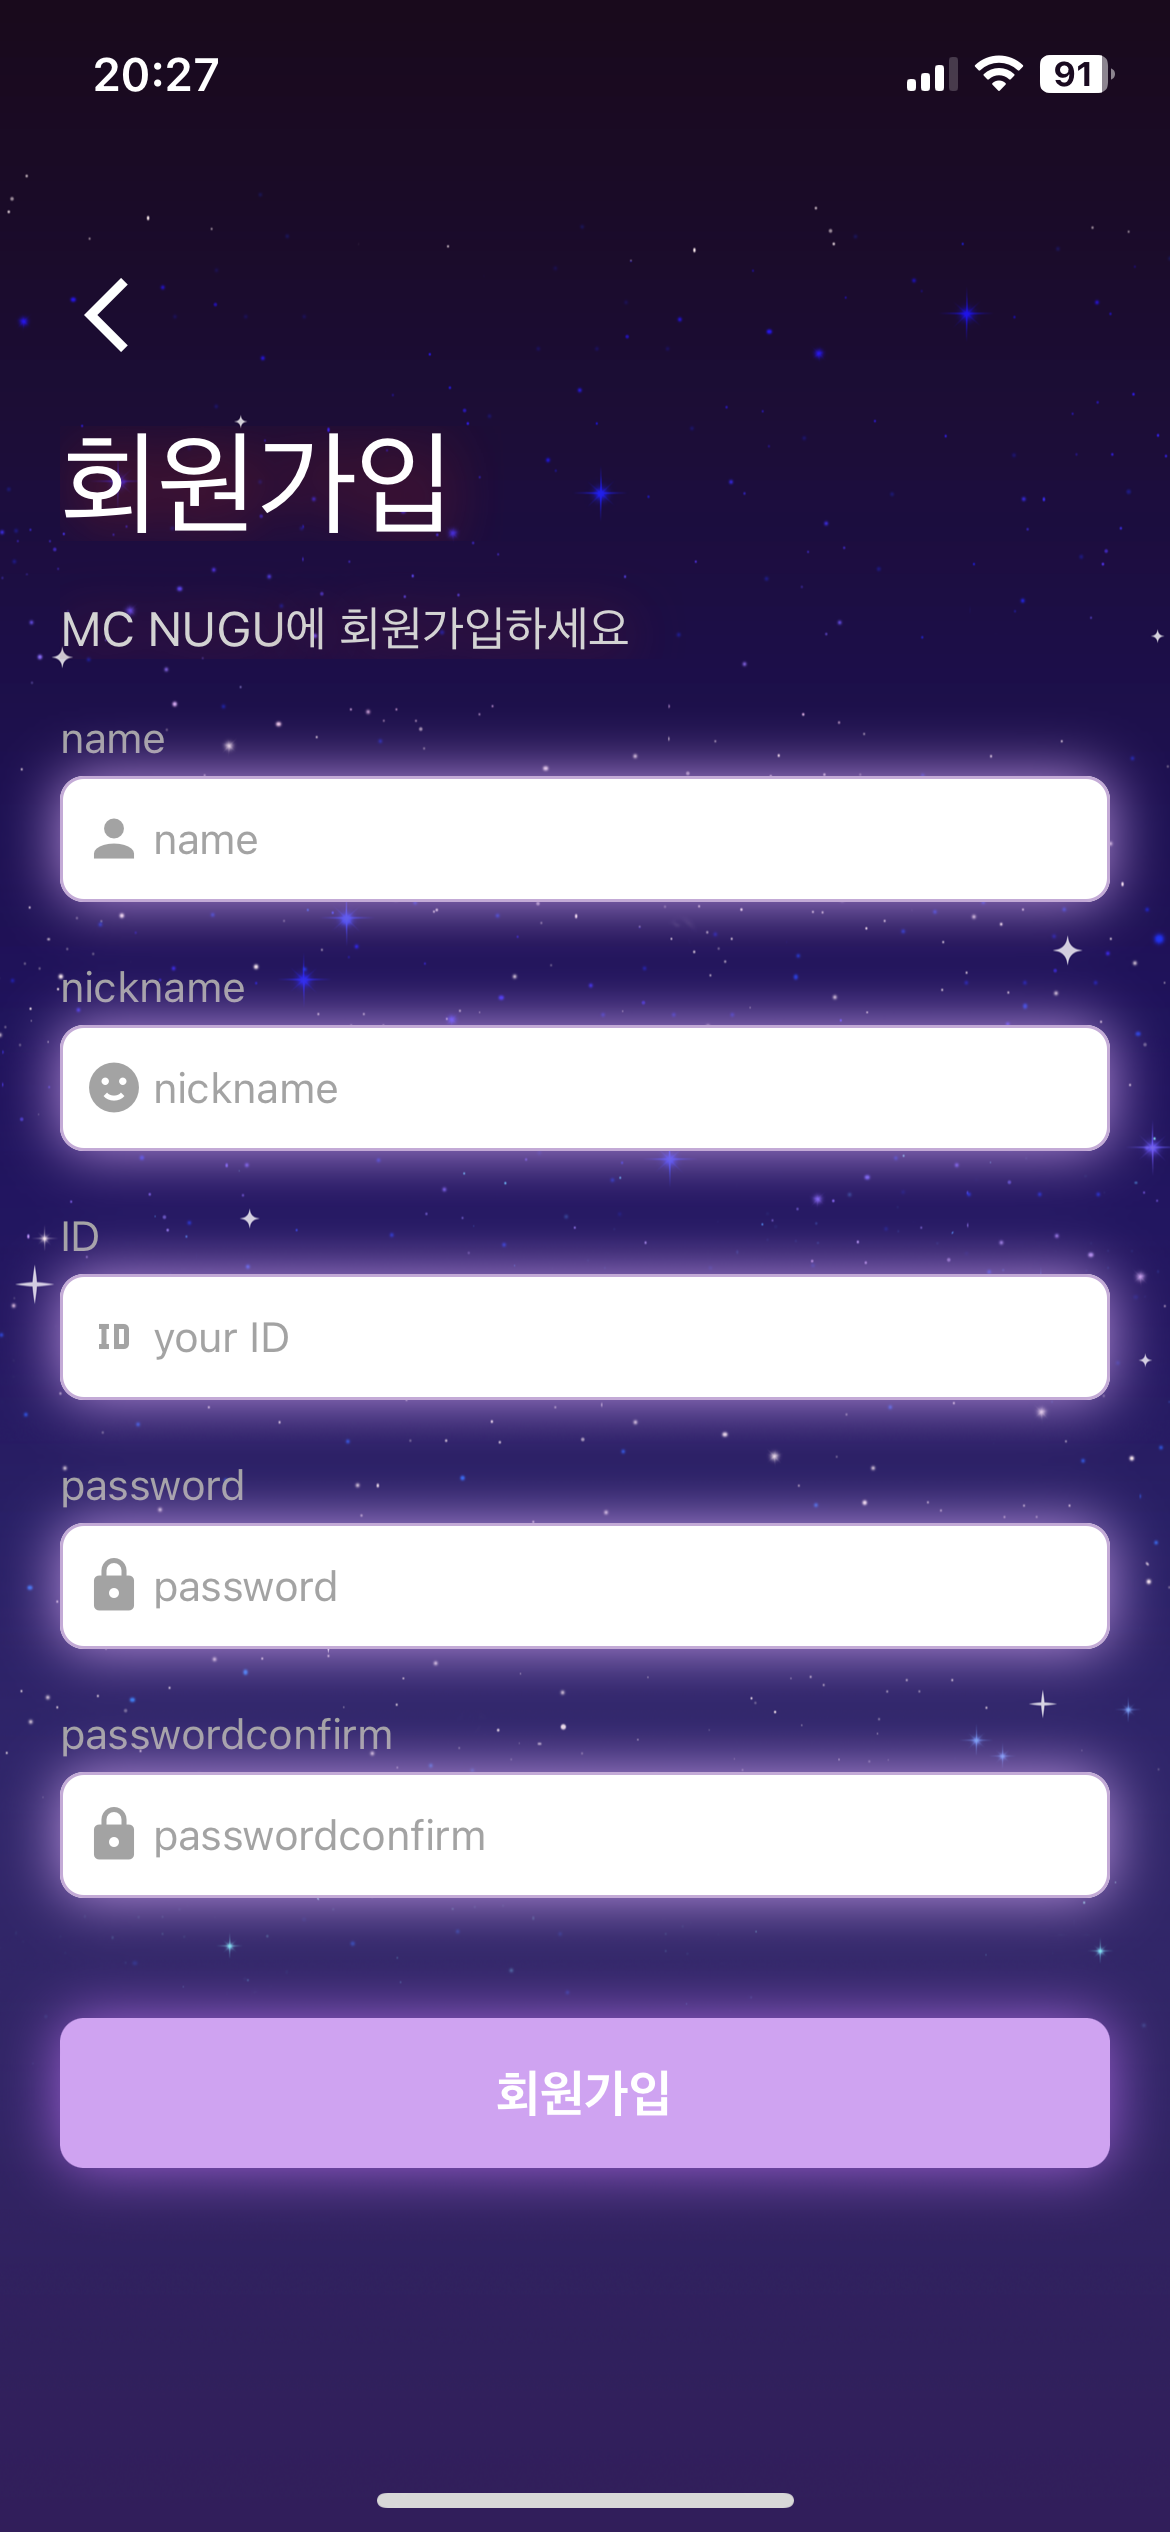
\includegraphics[width=3cm]{Images/screen/signup/SIGNUP_EMPTY.PNG}}
            \caption{Register Page}
            \label{fig}
        \end{figure}
        Users can sign up by setting a user id and password of their preference. Signing in requires input  of the given information in the sign up process such as user id, password and name. There are boxes for input of the ID, name, nickname, password and password check. ID is the one that should be input in the login process, name refers to real name, nickname will be the name that will be shown to other users, password is also used in the login process and password check is used to double check if the user made their password as intended.\\
        Initially, on the client side, there are character limits and a check to ensure that the password and password check fields match. Once the client-side validation is successful, the client sends these fields to the server because client-side checks can be easily bypassed. On the server side, there is a secondary validation for each field to check for errors. If there are no errors, the data is saved to the Member database.  \\
        For the UI which is similar to the login process, clicking on an input field highlights it, brings up the keyboard, and ensures that the keyboard doesn't cover the screen. Even if the user doesn't directly click on an input field, pressing the next button will move to the next input field. The password and password confirm fields are displayed in an encrypted format. If any of the fields (name, nickname, ID, password, password confirm) are left empty or if the password and password confirm do not match, the sign-up button remains inactive. Only when all input fields are correctly filled does the sign-up button become active. Upon successful registration, the screen transits to the login page. If registration fails, an alert message is displayed, and the user remains on the registration screen.
    \subsection{Space List Page}
        \begin{figure}[htbp]
            \centerline{
            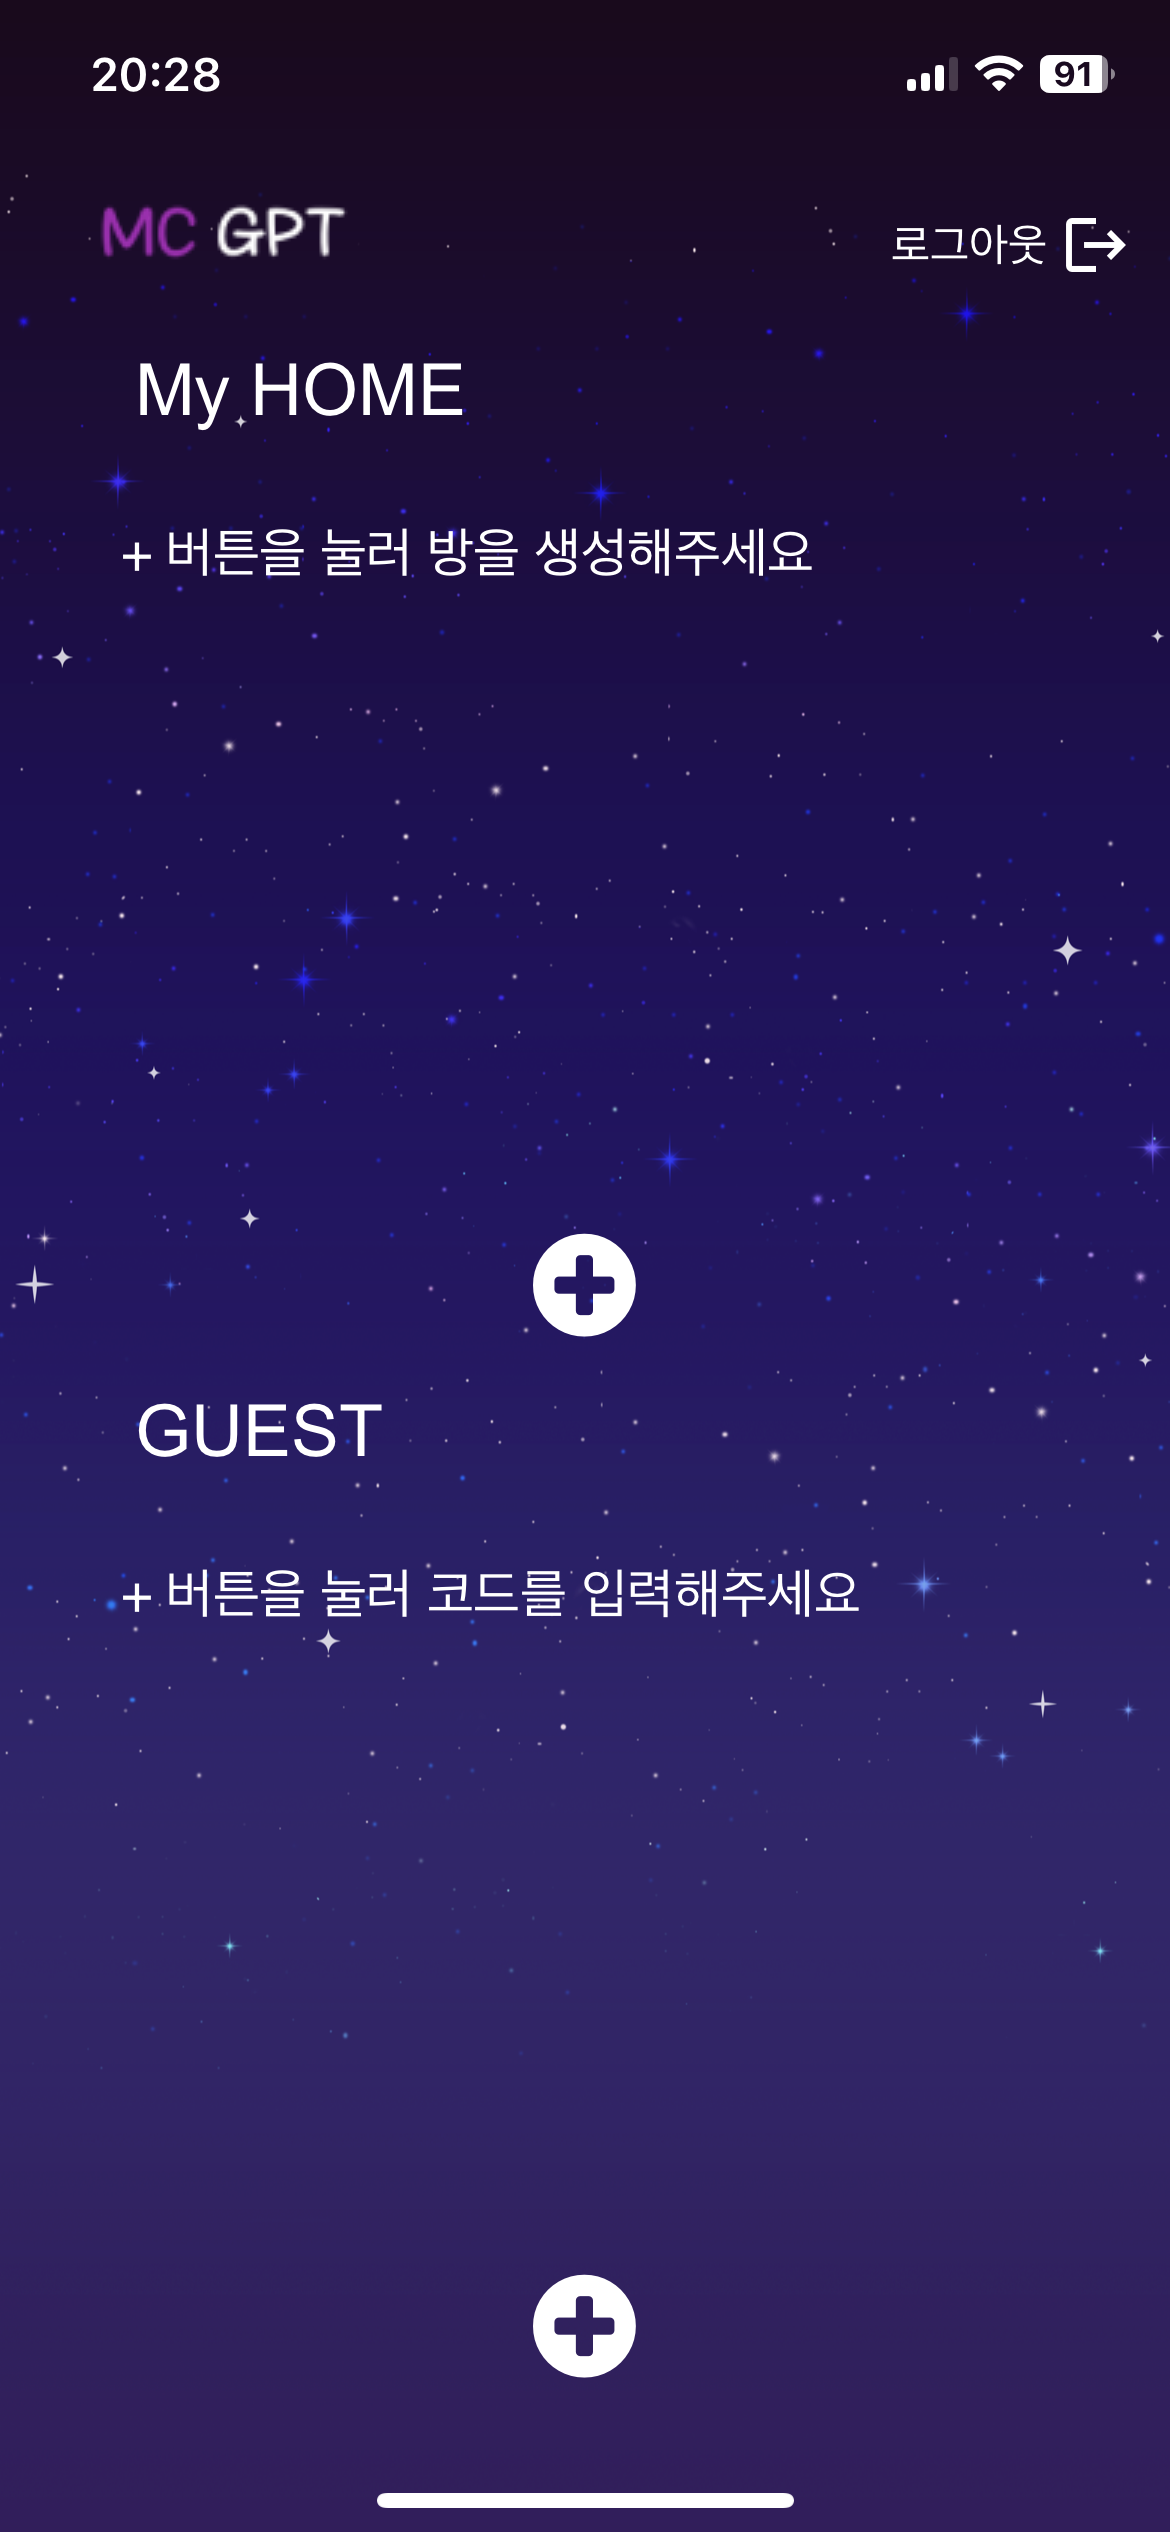
\includegraphics[width=3cm]{Images/screen/space/1_SPACE_EMPTY.PNG}
            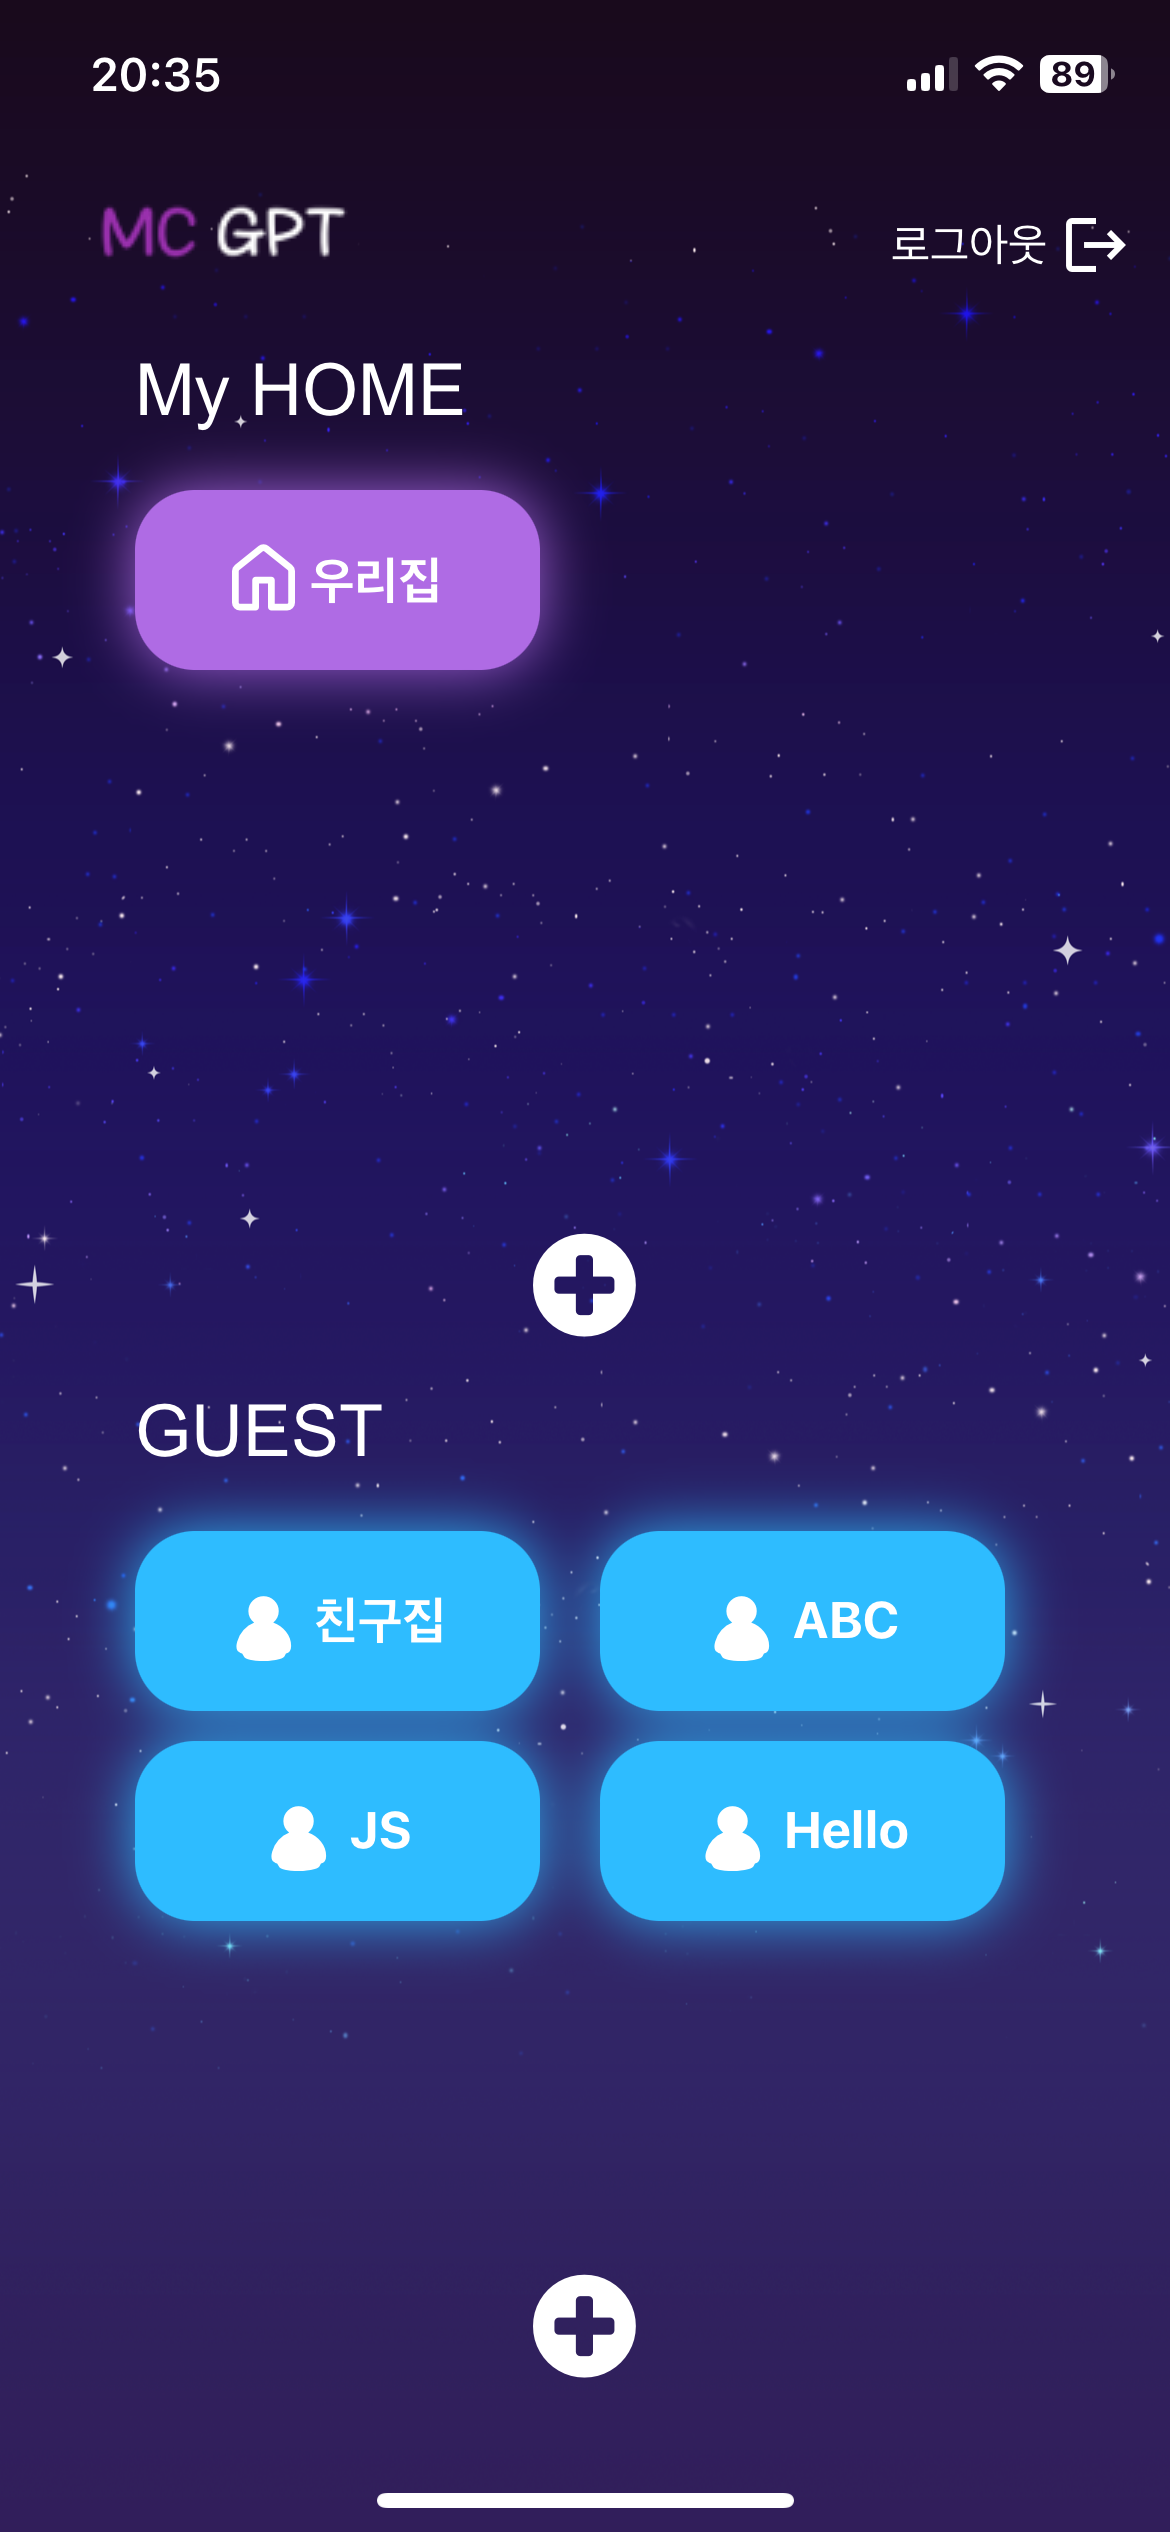
\includegraphics[width=3cm]{Images/screen/space/8_SPACE_FULL.PNG}}
            \caption{Space List Page}
            \label{fig}
        \end{figure}
        “Space” refers to any type of place where parties can be held and these spaces can be added to the application. Page with the list of spaces is where users can outlook the spaces that are registered to the app. It is divided into two parts; first is ‘My Home ', which is the list of spaces that are owned by the user and registered to the application. Second is ‘Guest’ which has a list of spaces that the users are as guests by inputting the entrance code of spaces. Also there are buttons to activate pop-ups that allow users to add a new space or a pop-up for guest users to input the space code they have received.\\
        The JWT, sent in the header, is decoded to extract the user's ID. Using this ID, both the list of spaces owned by the member and the list of spaces the member has joined as a guest are retrieved.\\
        On the screen, the space list is displayed in two columns, with a "My Home" section and a "Guest" section, clearly distinguishing between the spaces the member owns and the spaces they have joined as a guest.  Clicking the "Create Space" button opens a pop-up screen for creating a space, and clicking the "Enter Code" button opens a pop-up screen for entering a code to join an existing space. Space owners will see their spacess listed under "My Home," while guests will see records of the spaces they have joined under the "Guest" section.  Clicking the "Log Out" button will transition the screen back to the initial login screen.
    \subsection{Space Registration Pop-Up}
        \begin{figure}[htbp]
            \centerline{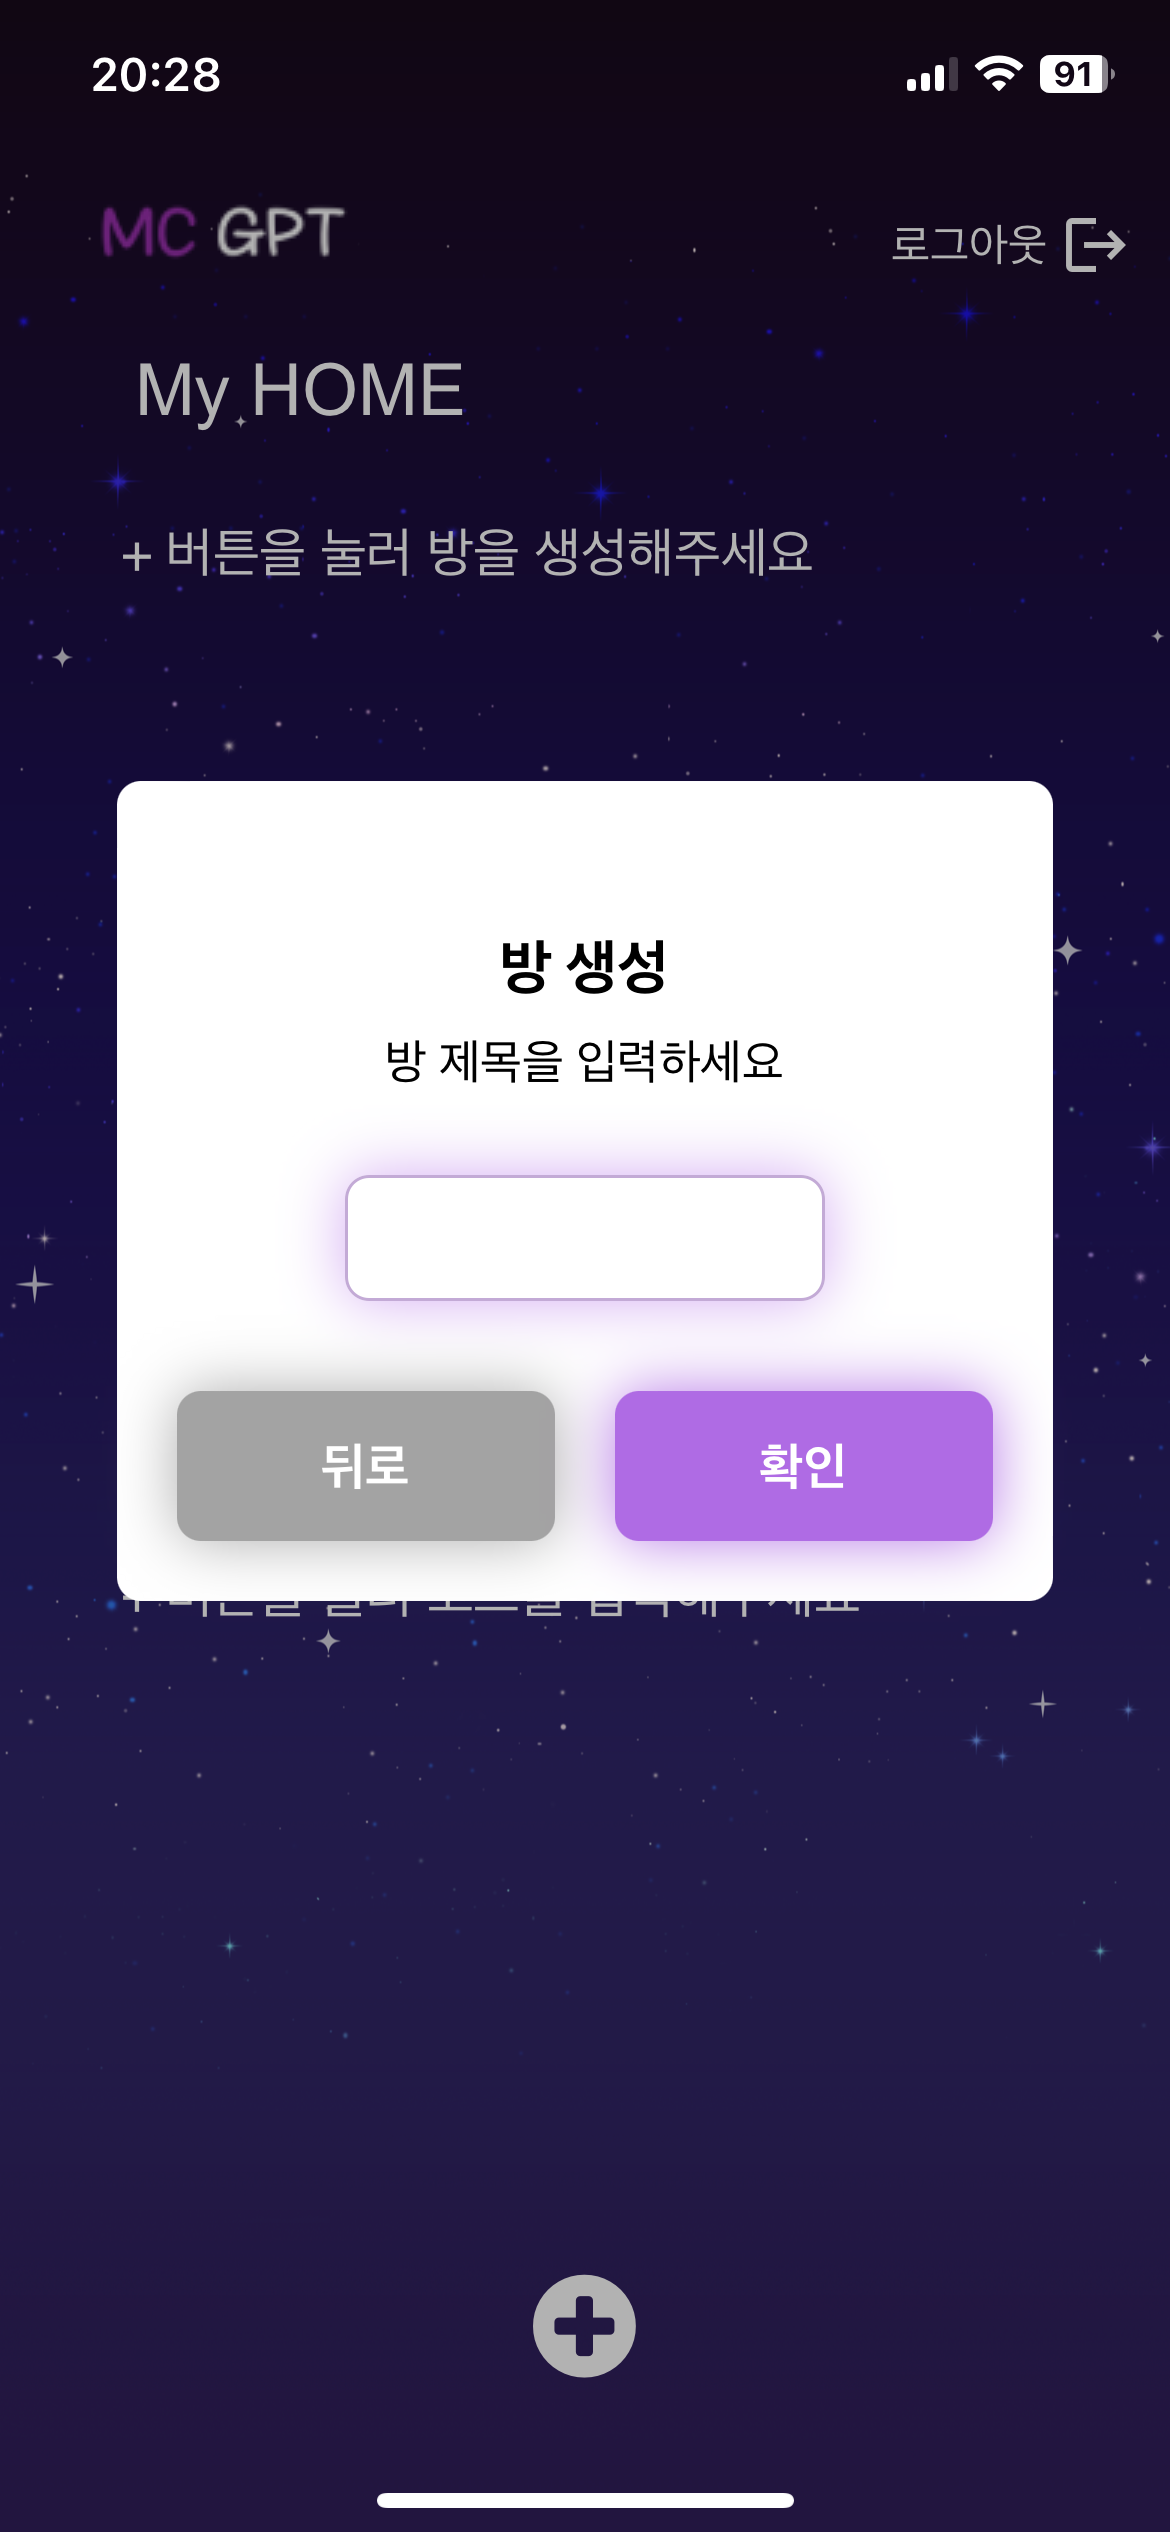
\includegraphics[width=3cm]{Images/screen/space/2_SPACE_POPUP1.PNG}}
            \caption{Space Registration Pop-Up}
            \label{fig}
        \end{figure}
        For a space to be ready to use in the application, it needs to be registered firsthand. The space registration pop-up can be accessed via the space list page. By activating the pop-up, space owners can input the name of the space and receive a invitation code for the space. After this process is valid, the new space should be added to the space list page.\\
        On the screen, the user inputs a room name, and a request is sent to the server to store it in the Home database. During this process, a room ID is generated along with a 4-digit random code that will be used for guest access. \\
        A pop-up screen for entering the space title is displayed. While this pop-up is open, the background of the room selection screen becomes opaque, and elements on the room selection screen cannot be interacted until the pop-up is closed. If the user clicks the "Back" button, they return to the space selection screen. If they enter a valid space title and click the "Confirm" button, a space is created, and the screen transitions to the Dashboard Page of the newly created space. If the space title is not entered correctly, a space creation failure alert is displayed, and the pop-up screen remains open.
    \subsection{Space Entrance Pop-Up}
        \begin{figure}[htbp]
            \centerline{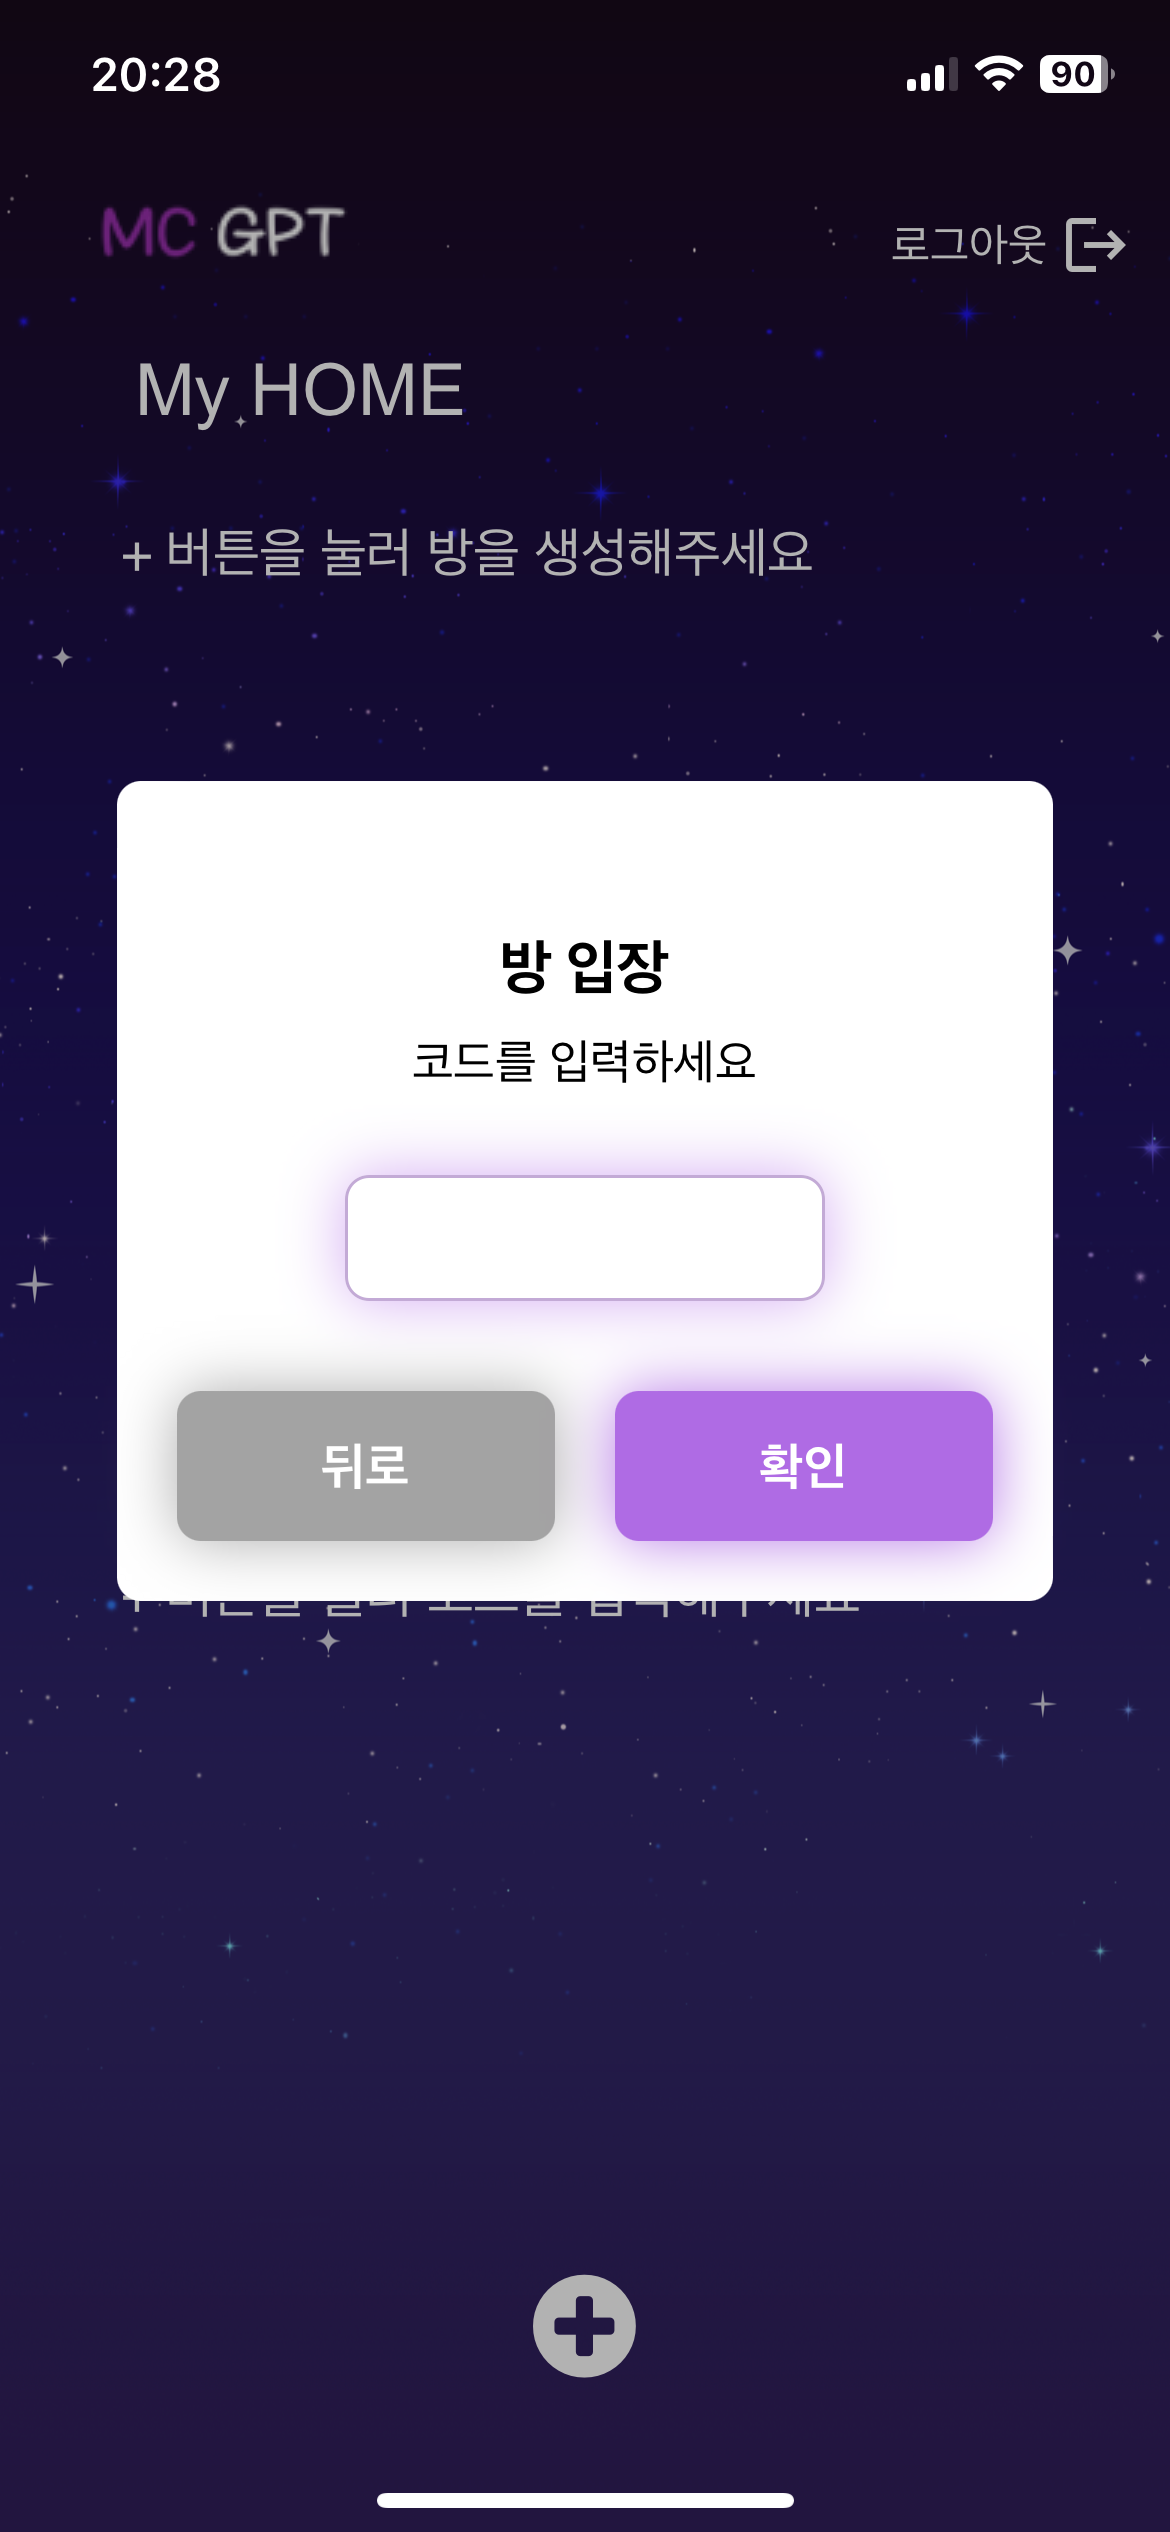
\includegraphics[width=3cm]{Images/screen/space/5_SPACE_POPUP2.PNG}}
            \caption{Space Entrance Pop-Up}
            \label{fig}
        \end{figure}
        Space entrance pop-up is the first step for guest users to be able to gain allowance to spaces. This pop-up can be accessed from the space list page.  A space user can gain access to spaces with the code provided by the owner. By having the code, the user also has access to the lighting and appliances pre-registered by the Space owner. Upon inserting a valid space code, it will add a new space to the guest section of the space list page. Now users are allowed on the spaces.\\
        On the screen, when a code is entered, a request is sent to the server. The server searches the Home database for a matching entry. It also retrieves the user's ID from the JWT and fetches Member information. Once a match is found, the server stores the relationship between the Home and the Member in the Guest database, marking the user as a guest in that particular space.\\
        The process for entering a space using a code is similar to the space creation pop-up. After entering a valid code and clicking the "Confirm" button, the user enters the corresponding space, and the initial page, the Dashboard Page, is displayed. If the code is not entered correctly, an alert message is shown, prompting the user to re-enter the code, and the pop-up screen remains open.
    \subsection{Dashboard (Main Page)}
        \begin{figure}[htbp]
            \centerline{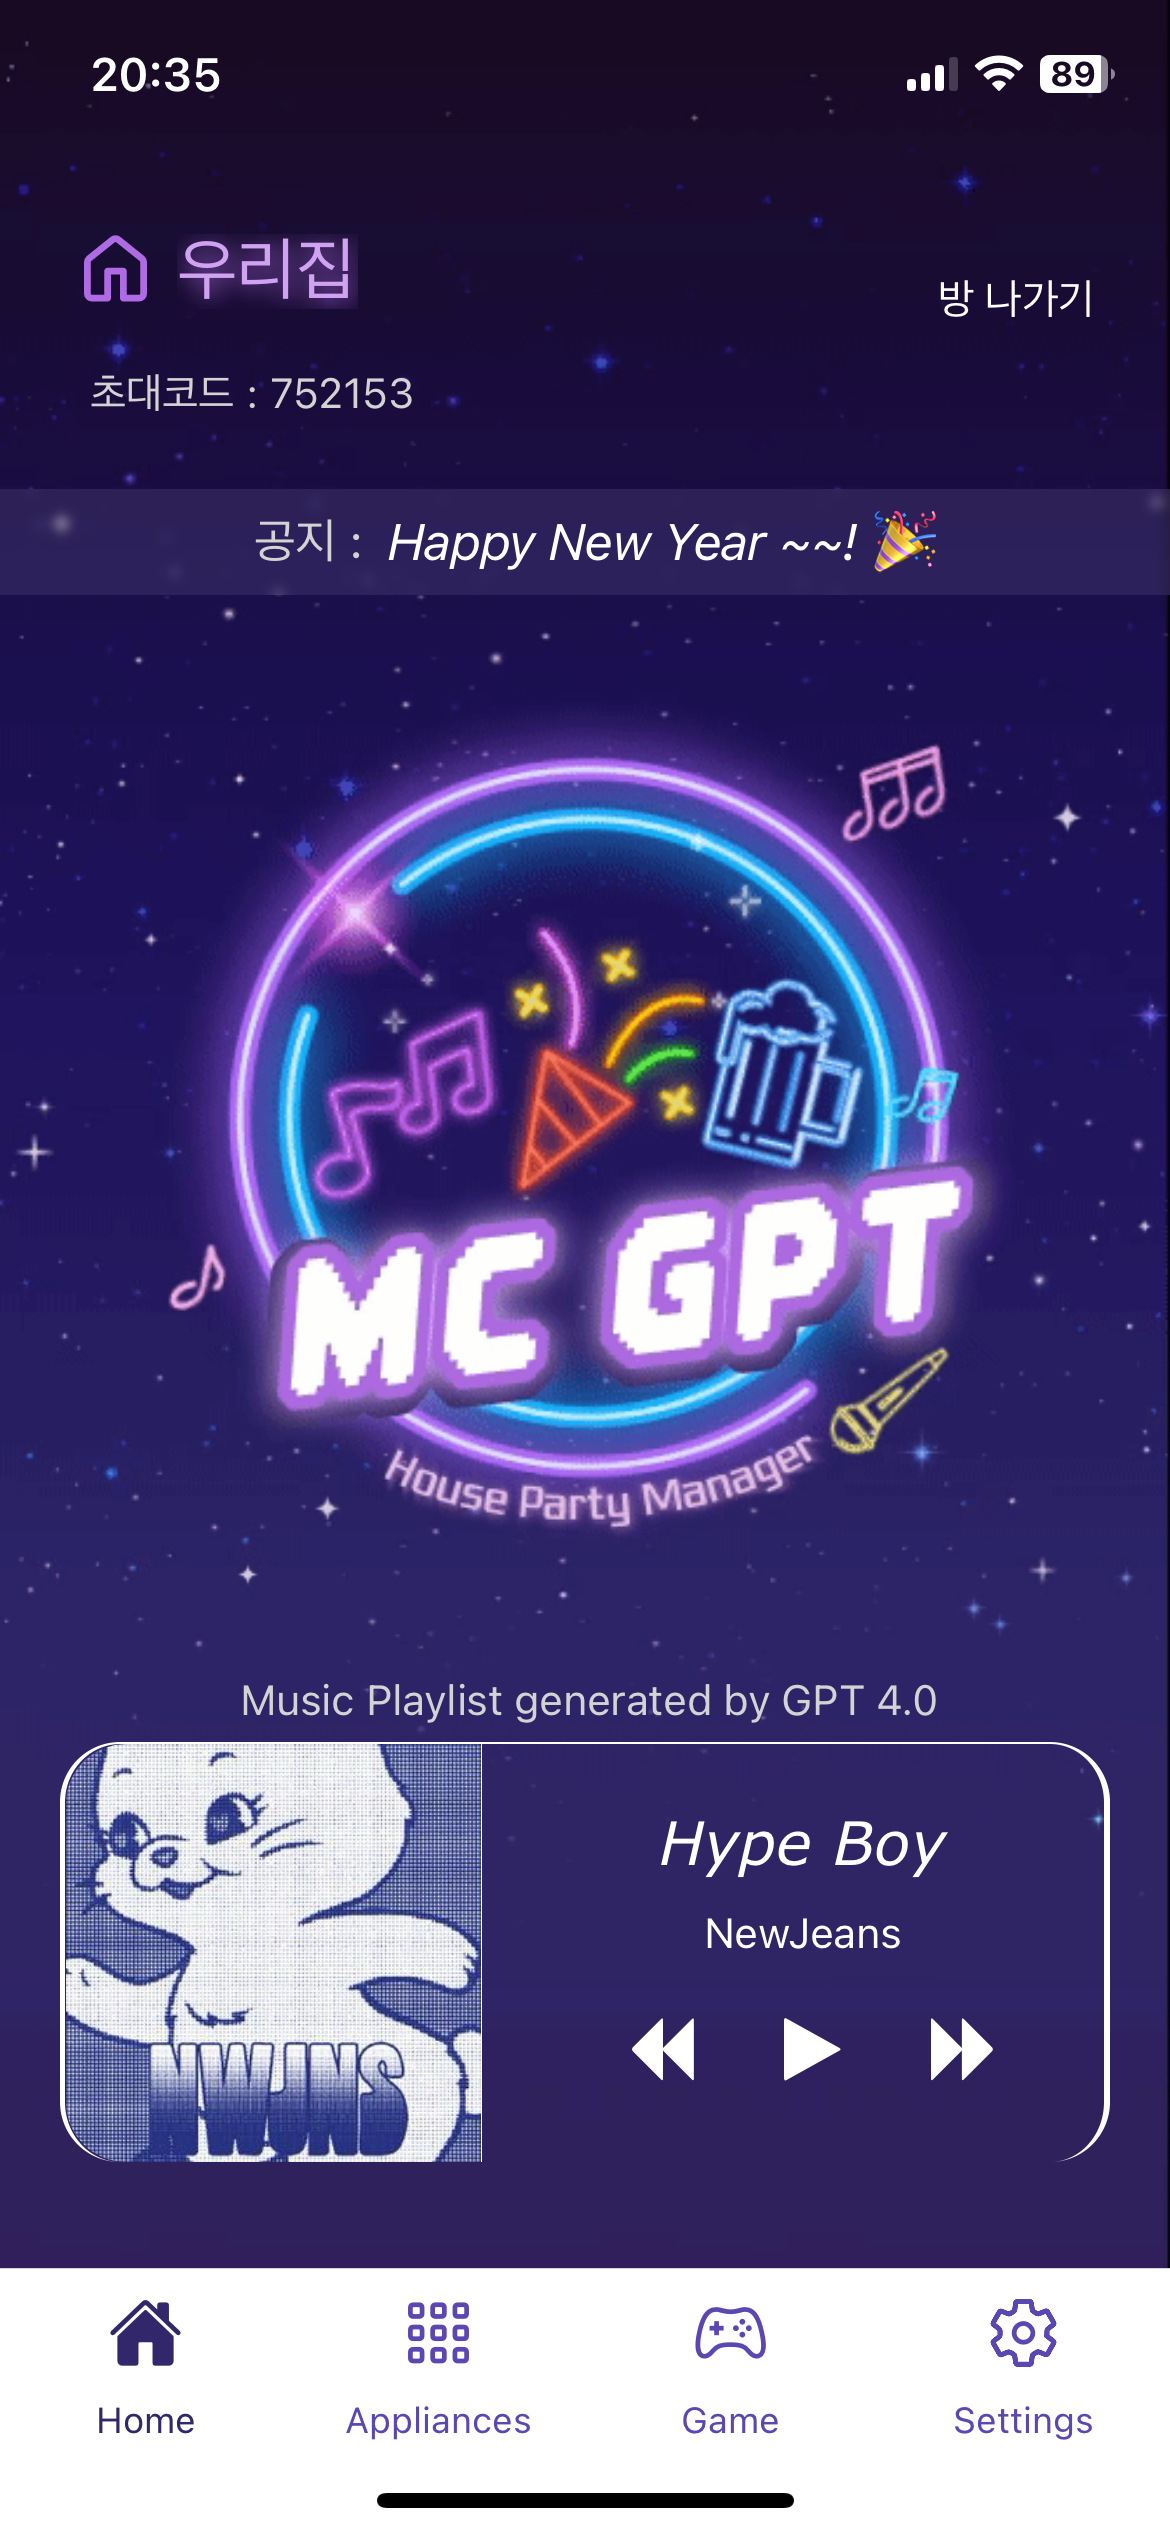
\includegraphics[width=3cm]{Images/screen/home/1_HOME_MYHOME.PNG}}
            \caption{Main Page}
            \label{fig}
        \end{figure}
        The Dashboard page is the main page that is first shown to users when entering a space. The main function of the dashboard page is showing an overview of the ongoing party. To help this objective, users can control the music playing from an audio device connected to the application, if there is any. Also there is a shared playlist where party participants can add desired songs to the list. In addition, there are information on the status of the space such as room temperature and air quality. These data can be sourced from the appliances that are connected to the space. Finally at the top there is the name of the space, exit space button, space code and a brief announcement bar. Name and code for the space is based on the data from the database and exiting button leads users back to the space list page. For the announcement bar, any user can post up to 25 characters and all users in the space can see the announcement.\\
        It's a screen composed of tabs, and from the user's perspective, it's not ideal to send requests every time you switch tabs, as it can cause delays. Therefore, as soon as you enter this screen, all the data for the space, including lighting and appliance lists, as well as the game list, is fetched all at once. This data is stored in a context for later use.\\        
        Announcements are displayed as text animations that move from the left side of the screen to the right side, taking 1 minute. There's a button to return to the room selection screen, allowing users to navigate back. On the screen, the album cover of the music currently playing on the AI speaker is displayed, along with music playback options and playlists.
    \subsection{Lighting \& Appliance Dashboard}
        \begin{figure}[htbp]
            \centerline{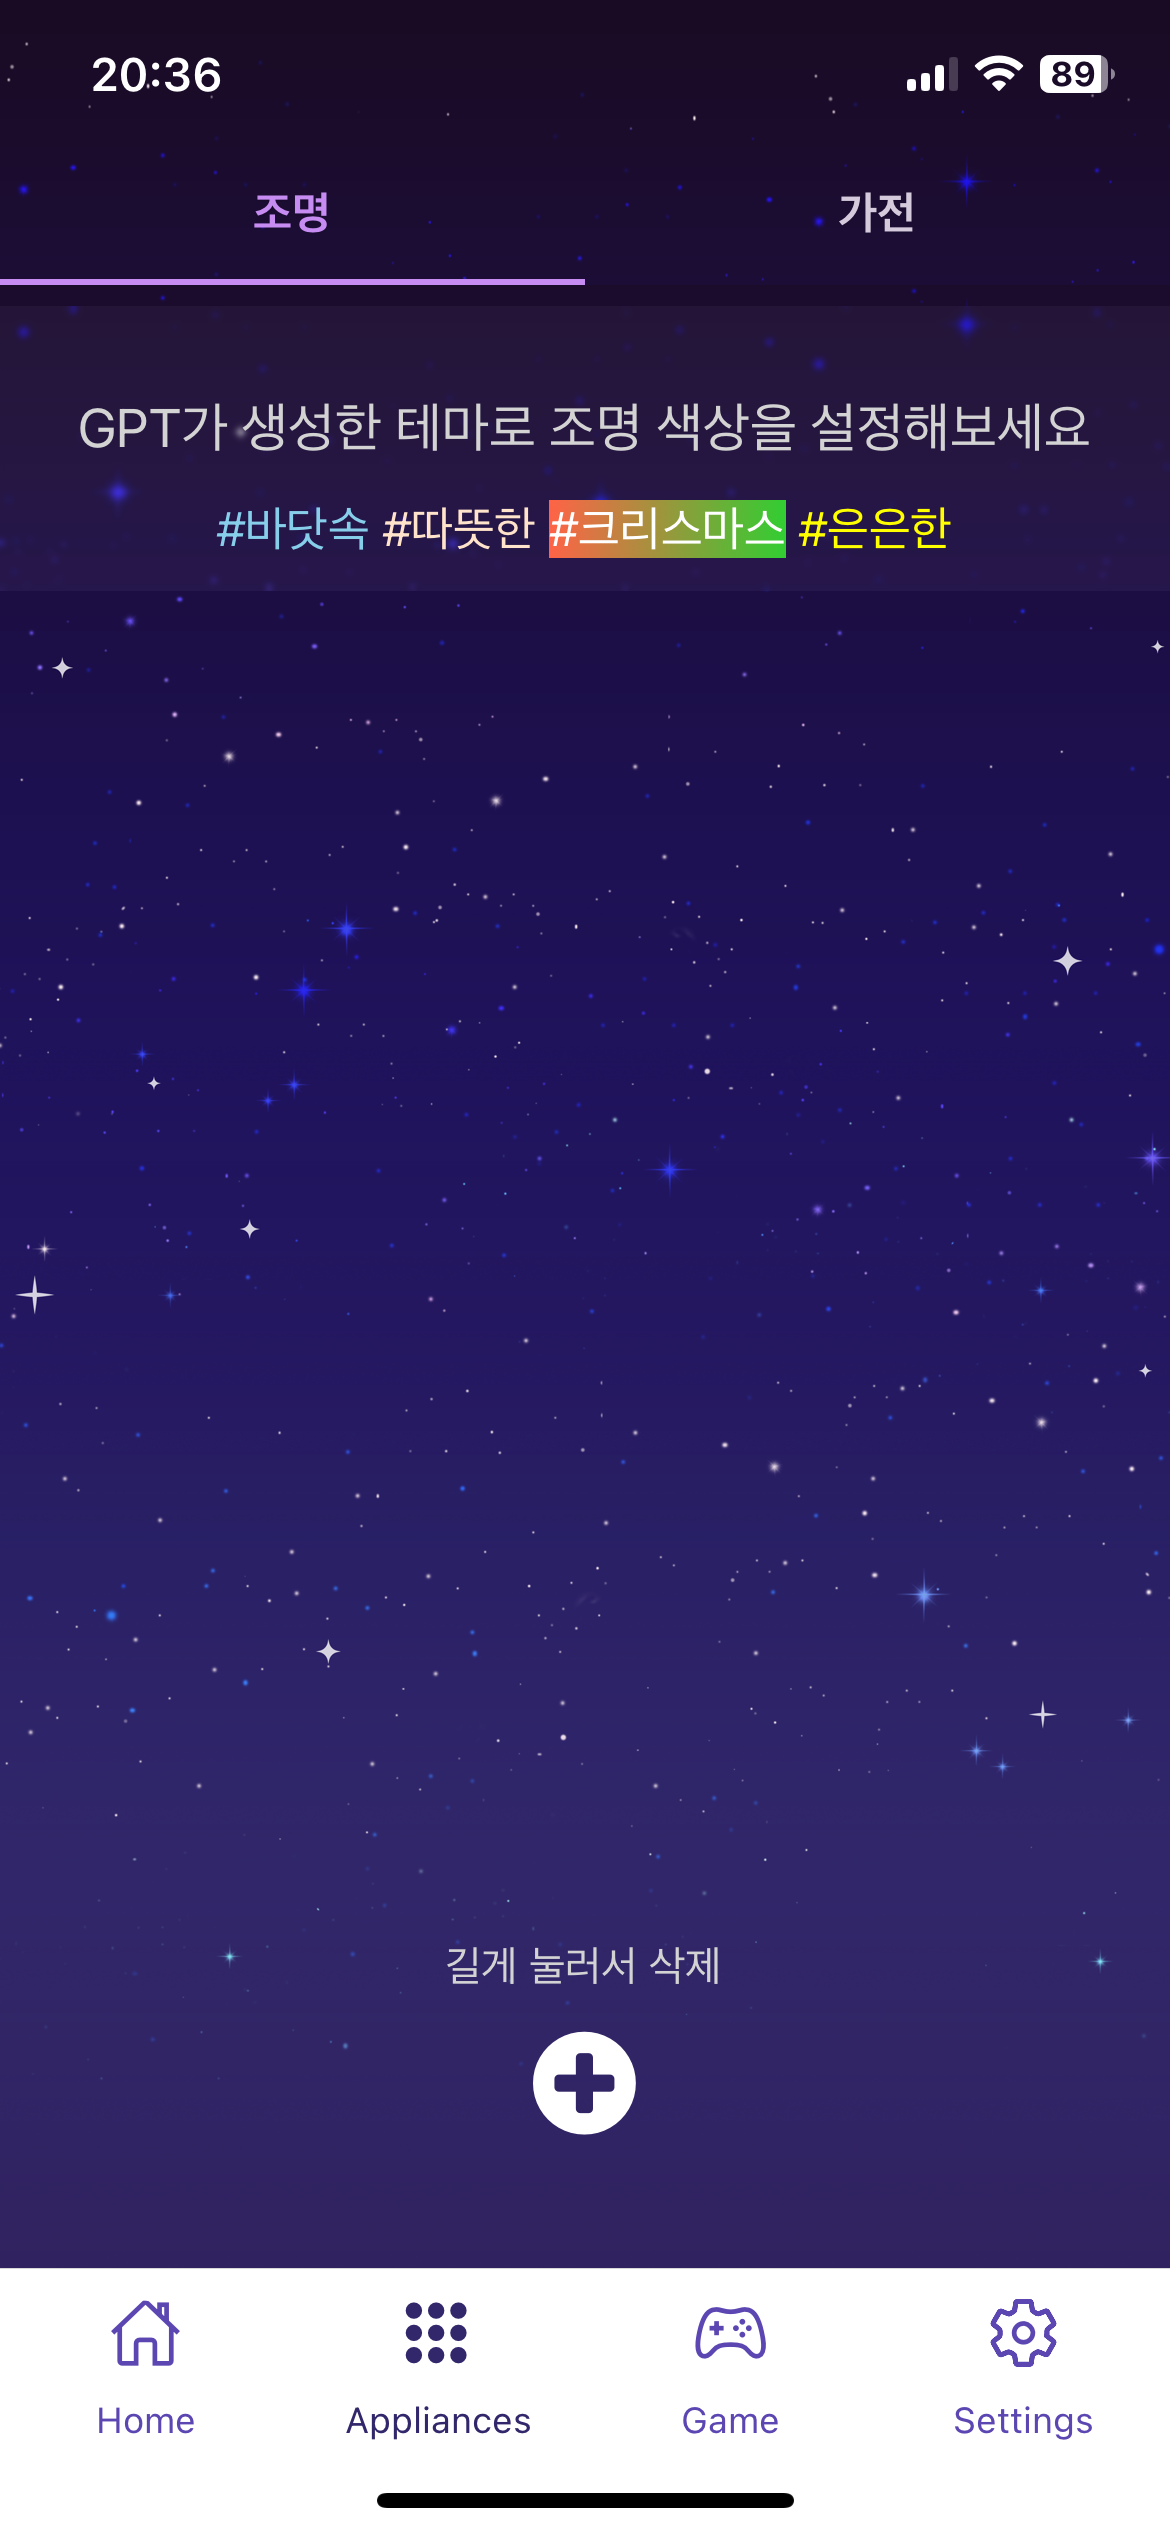
\includegraphics[width=3cm]{Images/screen/light/1_LIGHT_EMPTY.PNG}
            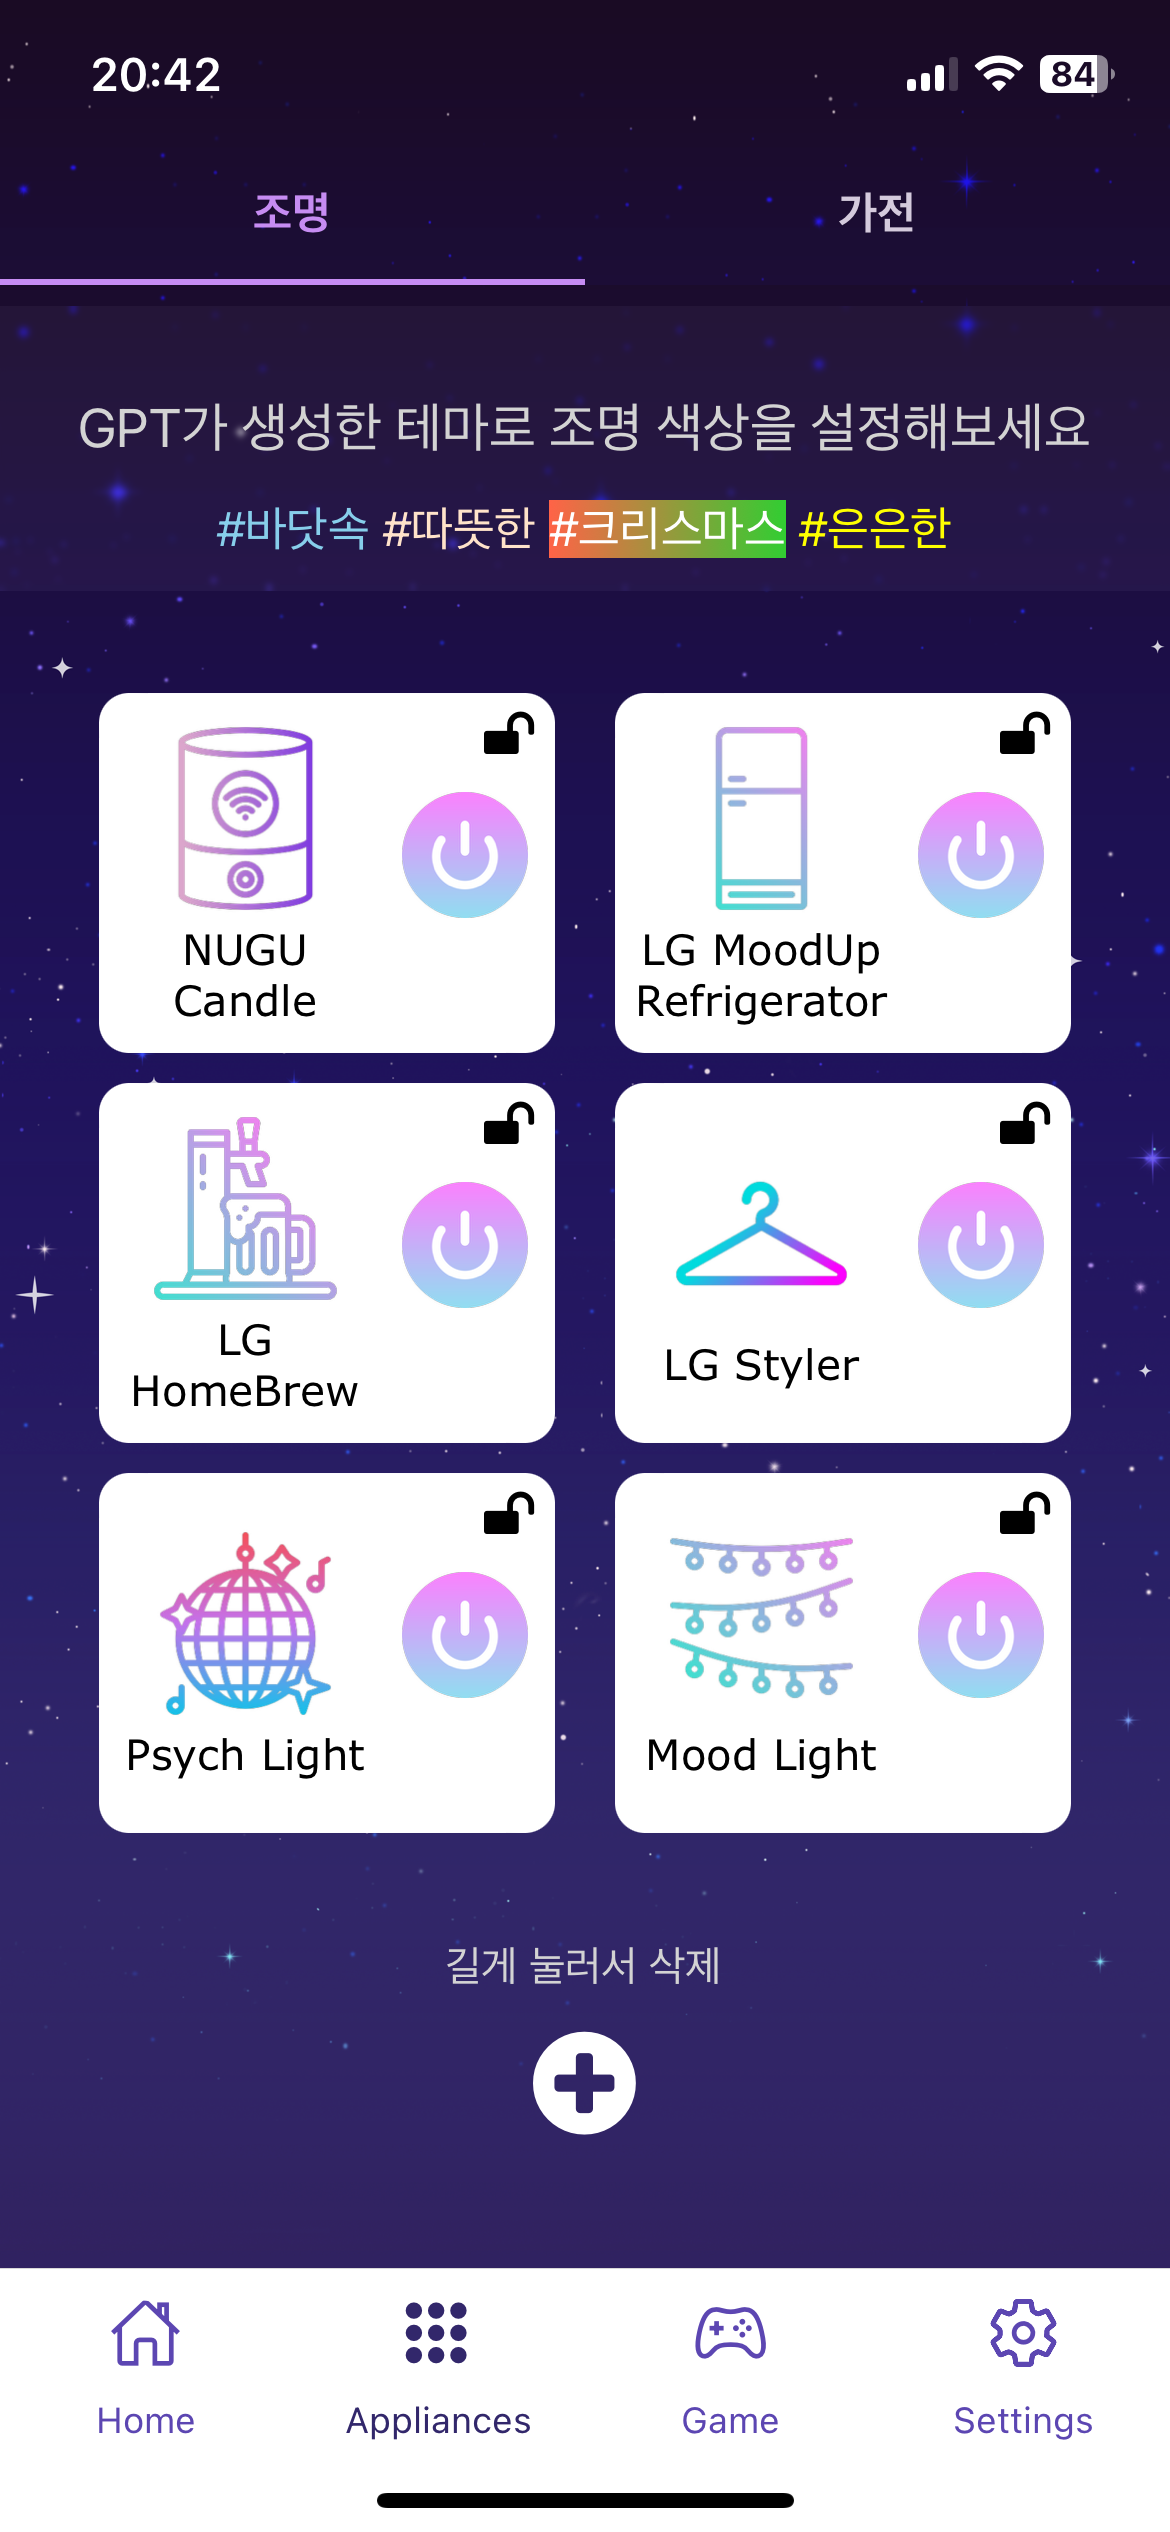
\includegraphics[width=3cm]{Images/screen/light/5_LIGHT_FULL.PNG}
            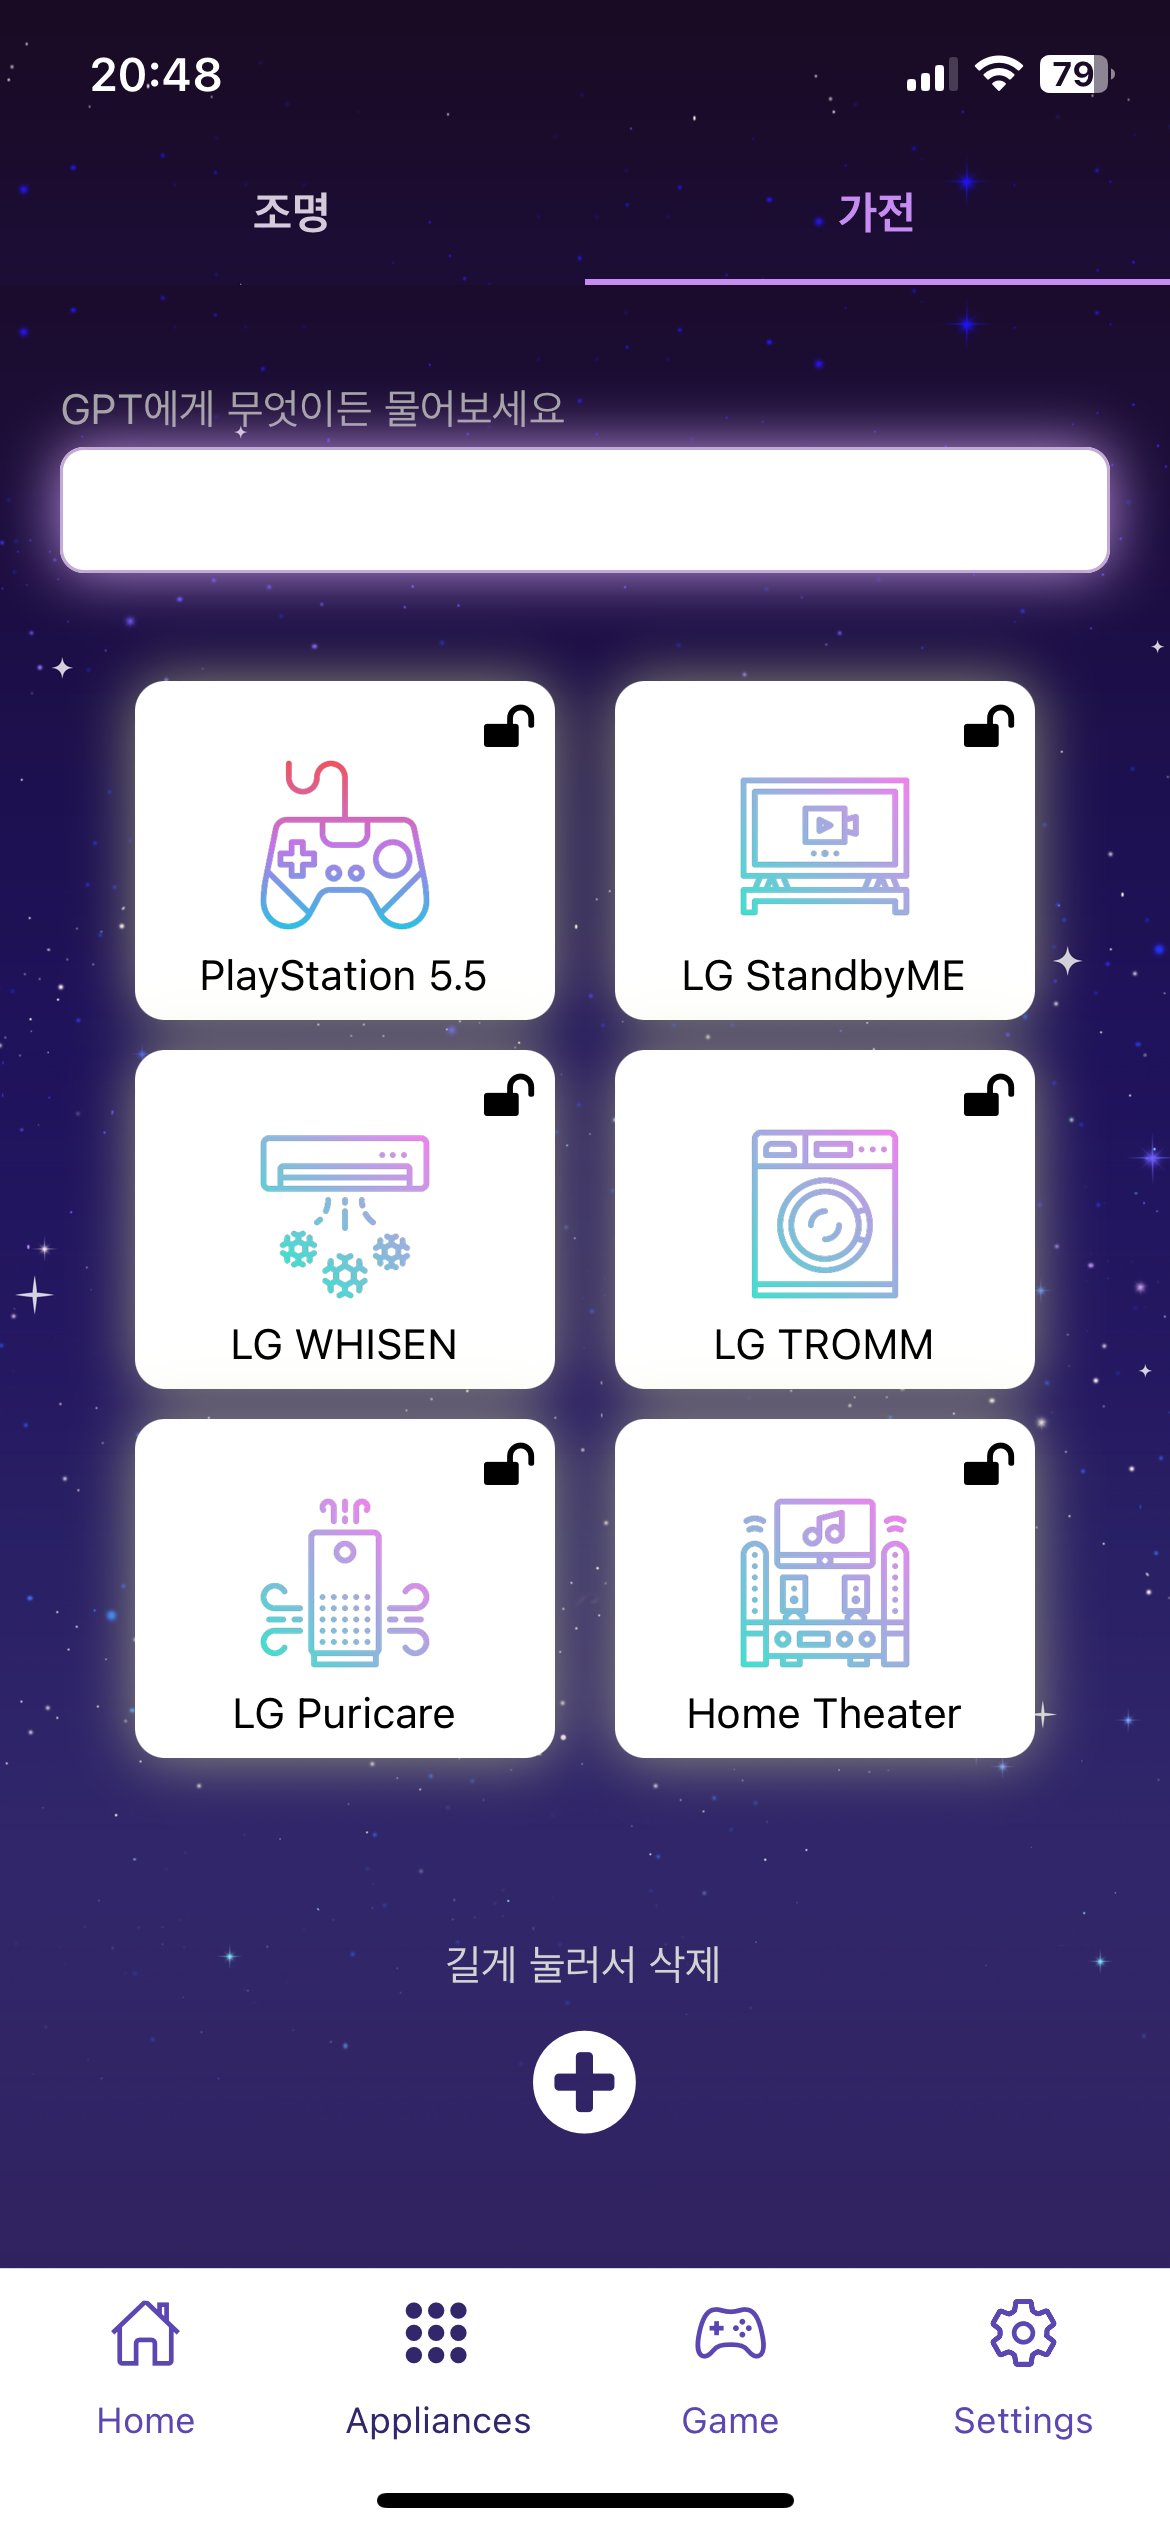
\includegraphics[width=3cm]{Images/screen/elec/5_ELEC_FULL.PNG}}
            \caption{Lighting \& Appliance Dashboard}
            \label{fig}
        \end{figure} 
        The appliance tab is the second tab of the application, which has functions that controls the appliances that are connected by the owner. The appliances are categorized into two groups: those with lighting and those without lighting. This page can give an overview of all the lighting and non-lighting appliances of the space. The dashboard consists of 2 identical pages for each type of appliance.\\
        In the Lighting tab, only appliances with the "light" variable set to true in the appliance list data are displayed.  Users can enter their desired ambiance in an input field, and based on the current number of people in the space and the ambiance input, they receive lighting RGB values and effects recommendations from a generative AI. These recommendations are then transmitted to all the lights using Matter for configuration.\\
        In the appliance tab, appliances without lighting features are able to be controlled. The specific functions vary on what type of appliances are added to the tab. It will be specified on later specifications but one example could be a temperature adjustment for an air conditioner.\\
        All appliance buttons are displayed on the screen in two columns and support simple on/off functionality. Tapping each appliance button takes the user to a detailed control screen for each individual appliance. By using the tabs at the top of the screen, users can switch to a screen for controlling appliances without lighting. "Add Lighting" or "Add Appliance" button allows users to add new appliances. Users can enter the desired lighting in an input field and, by pressing the keyboard's completion button, can obtain suitable lighting effects through OpenAI API and the server.

    \subsection{Lighting Device \& Appliance Registration Pop-Up}
        \begin{figure}[htbp]
            \centerline{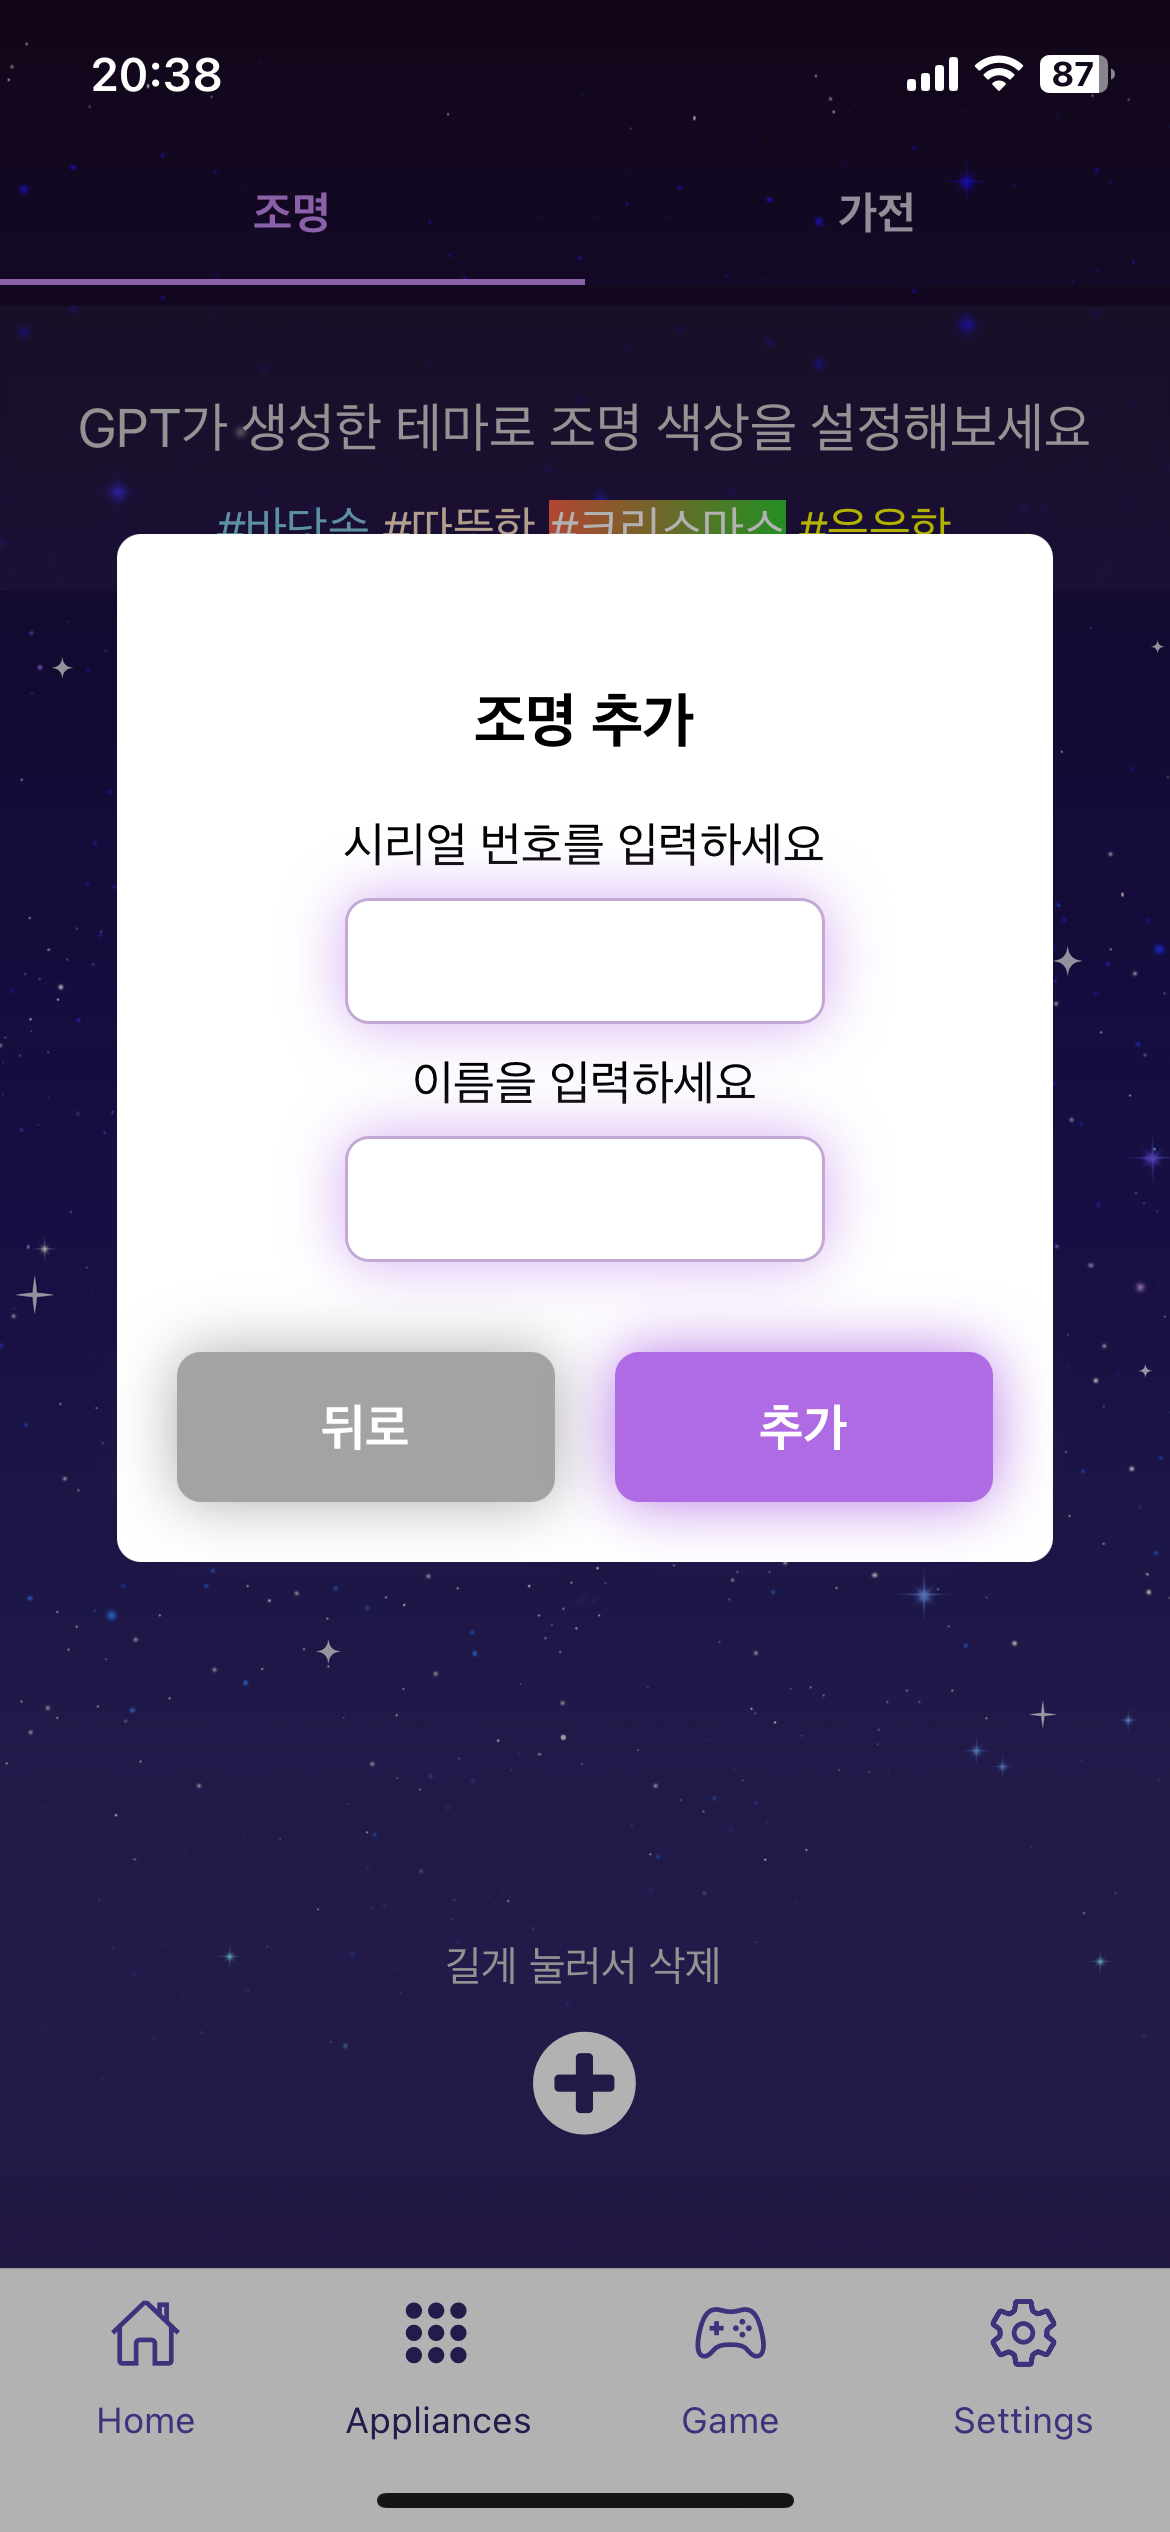
\includegraphics[width=3cm]{Images/screen/light/2_LIGHT_ADD_EMPTY.PNG}
            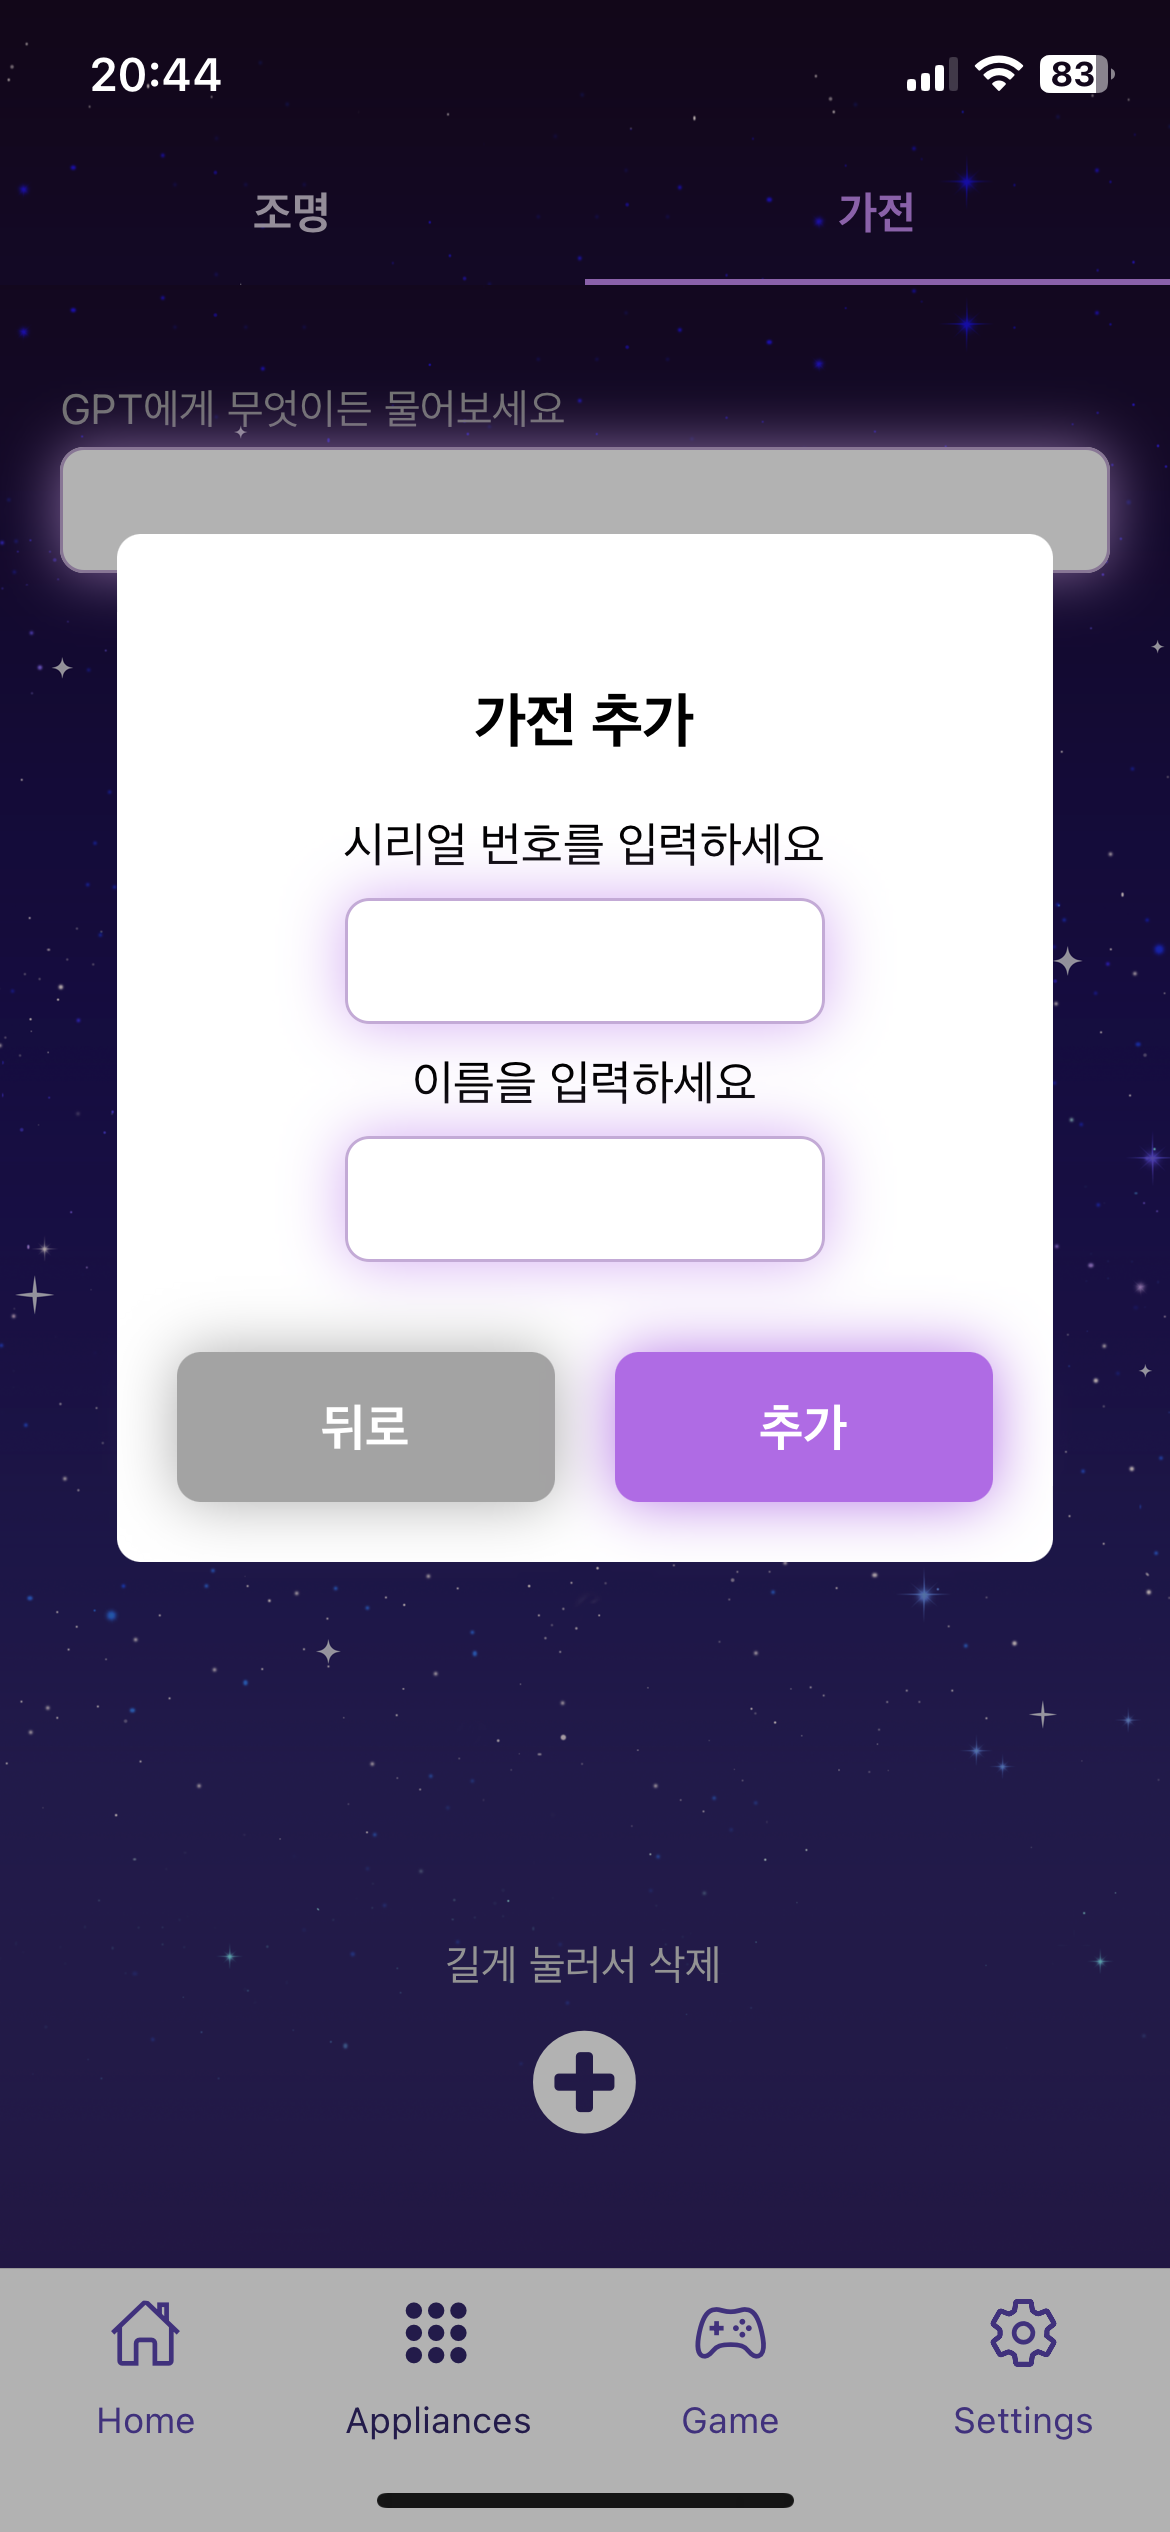
\includegraphics[width=3cm]{Images/screen/elec/2_ELEC_ADD_EMPTY.PNG}}
            \caption{Light \ & Appliance Registration}
            \label{fig}
        \end{figure}
        In order to control the appliances from the app, it needs to be registered initially. The registration pop-up will receive information about appliances from the owner ultimately sending the data to the server. Information needed for registration are the serial numbers and name of appliance. In an input bar on the pop-up serial numbers and names are entered. The server automatically categorizes the appliance based on the serial number, checking if it has lighting or determining its type.\\
        Tapping the serial number input field brings up the numerical keyboard, while tapping the name input field displays the Korean keyboard. The "Back" button allows users to return to the lighting screen, and after entering the information correctly, clicking the "Confirm" button results in the creation of a new lighting appliance. If the information is not entered correctly, the lighting appliance is not created, and a "Lighting(Appliance) Creation Failure" alert message is displayed.

    \subsection{Lighting Control Page}
        \begin{figure}[htbp]
            \centerline{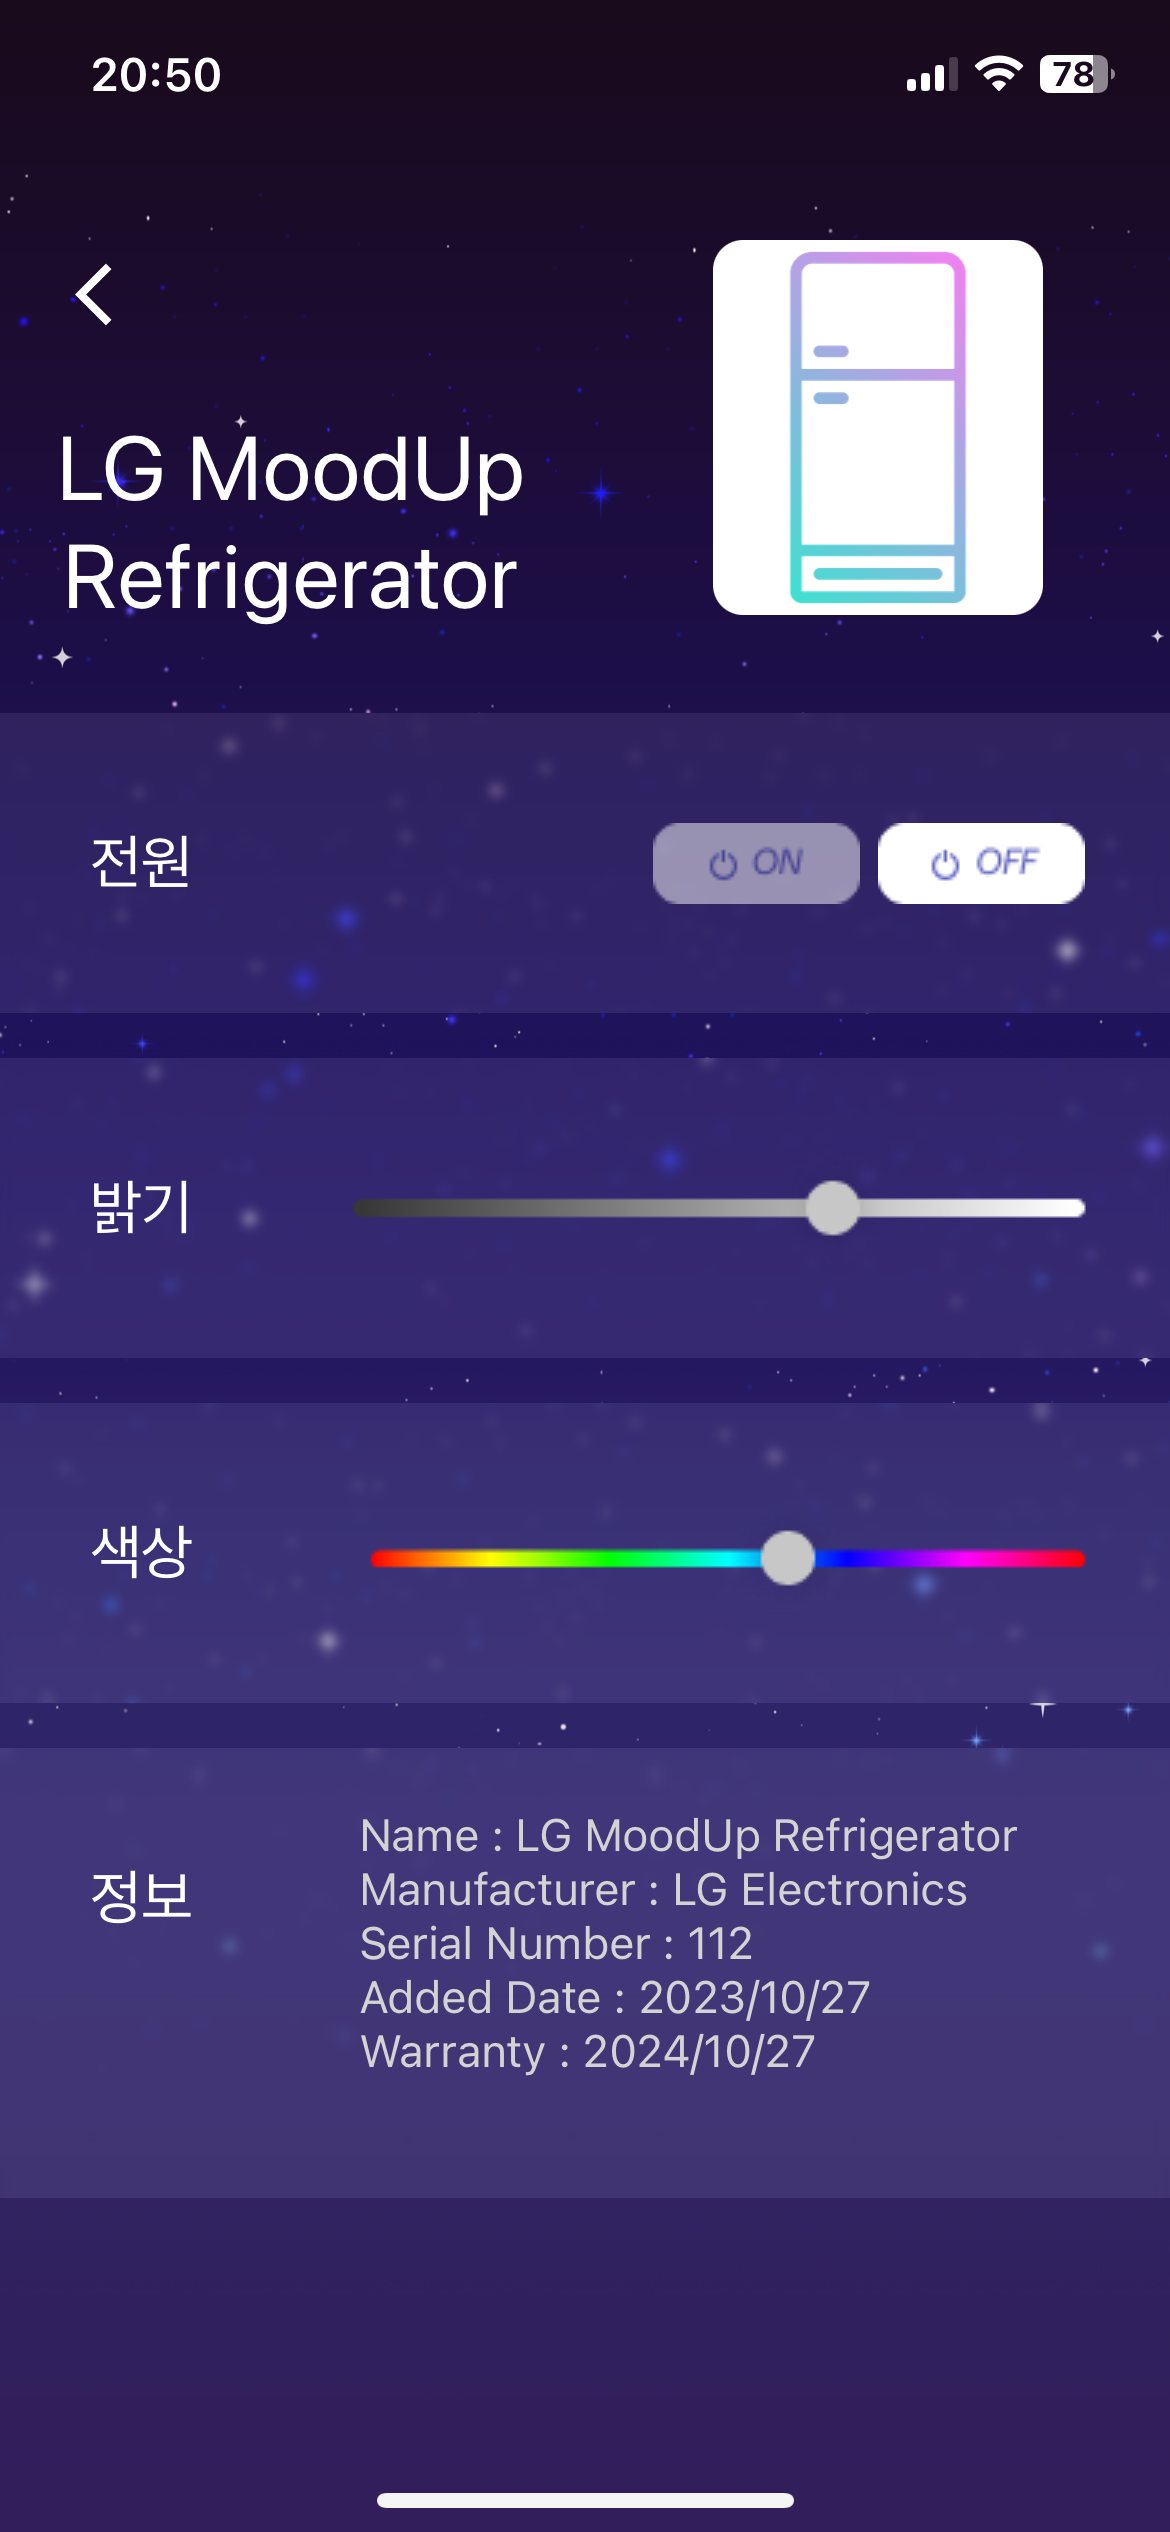
\includegraphics[width=3cm]{Images/screen/light/8_LIGHT_SETTING.PNG}
            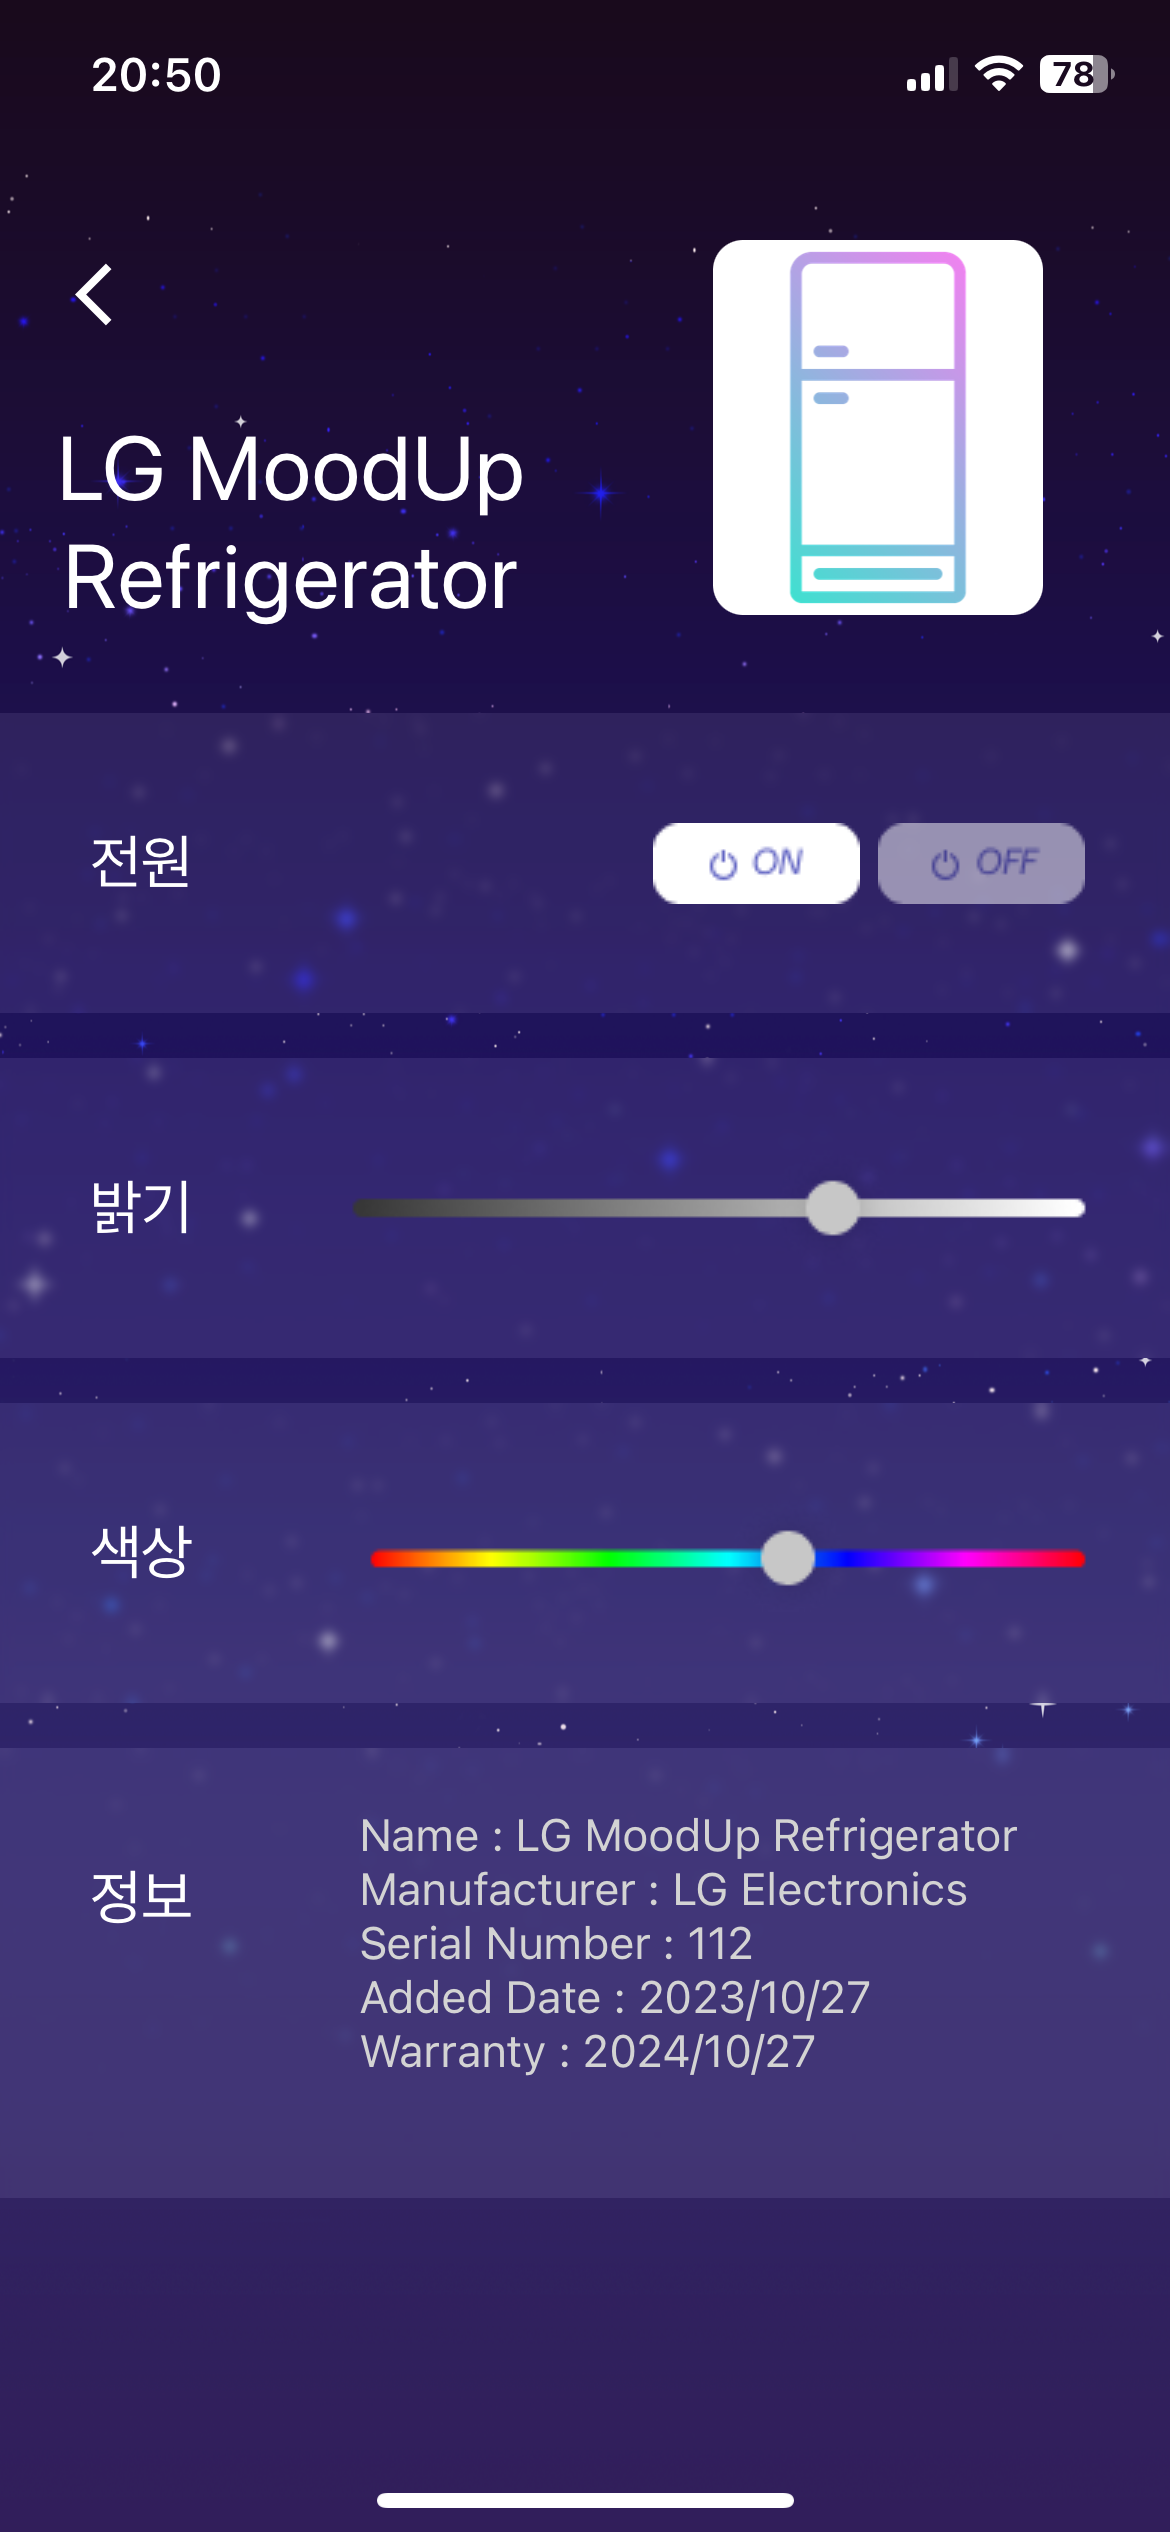
\includegraphics[width=3cm]{Images/screen/light/9_LIGHT_SETTING_ON.PNG}}
            \caption{Light Control}
            \label{fig}
        \end{figure}
        Using a standardized format with Matter, the frontend sends requests to the appliance in a structured format based on the input it receives.\\
        This screen allows you to control detailed lighting effects for appliances with lighting. At the top of the screen, the icon and name of the selected lighting appliance are displayed. You can control not only the on/off function of the lighting appliance but also check and modify features such as color, brightness, and usage.

    \subsection{Appliance Control Page}
        \begin{figure}[htbp]
            \centerline{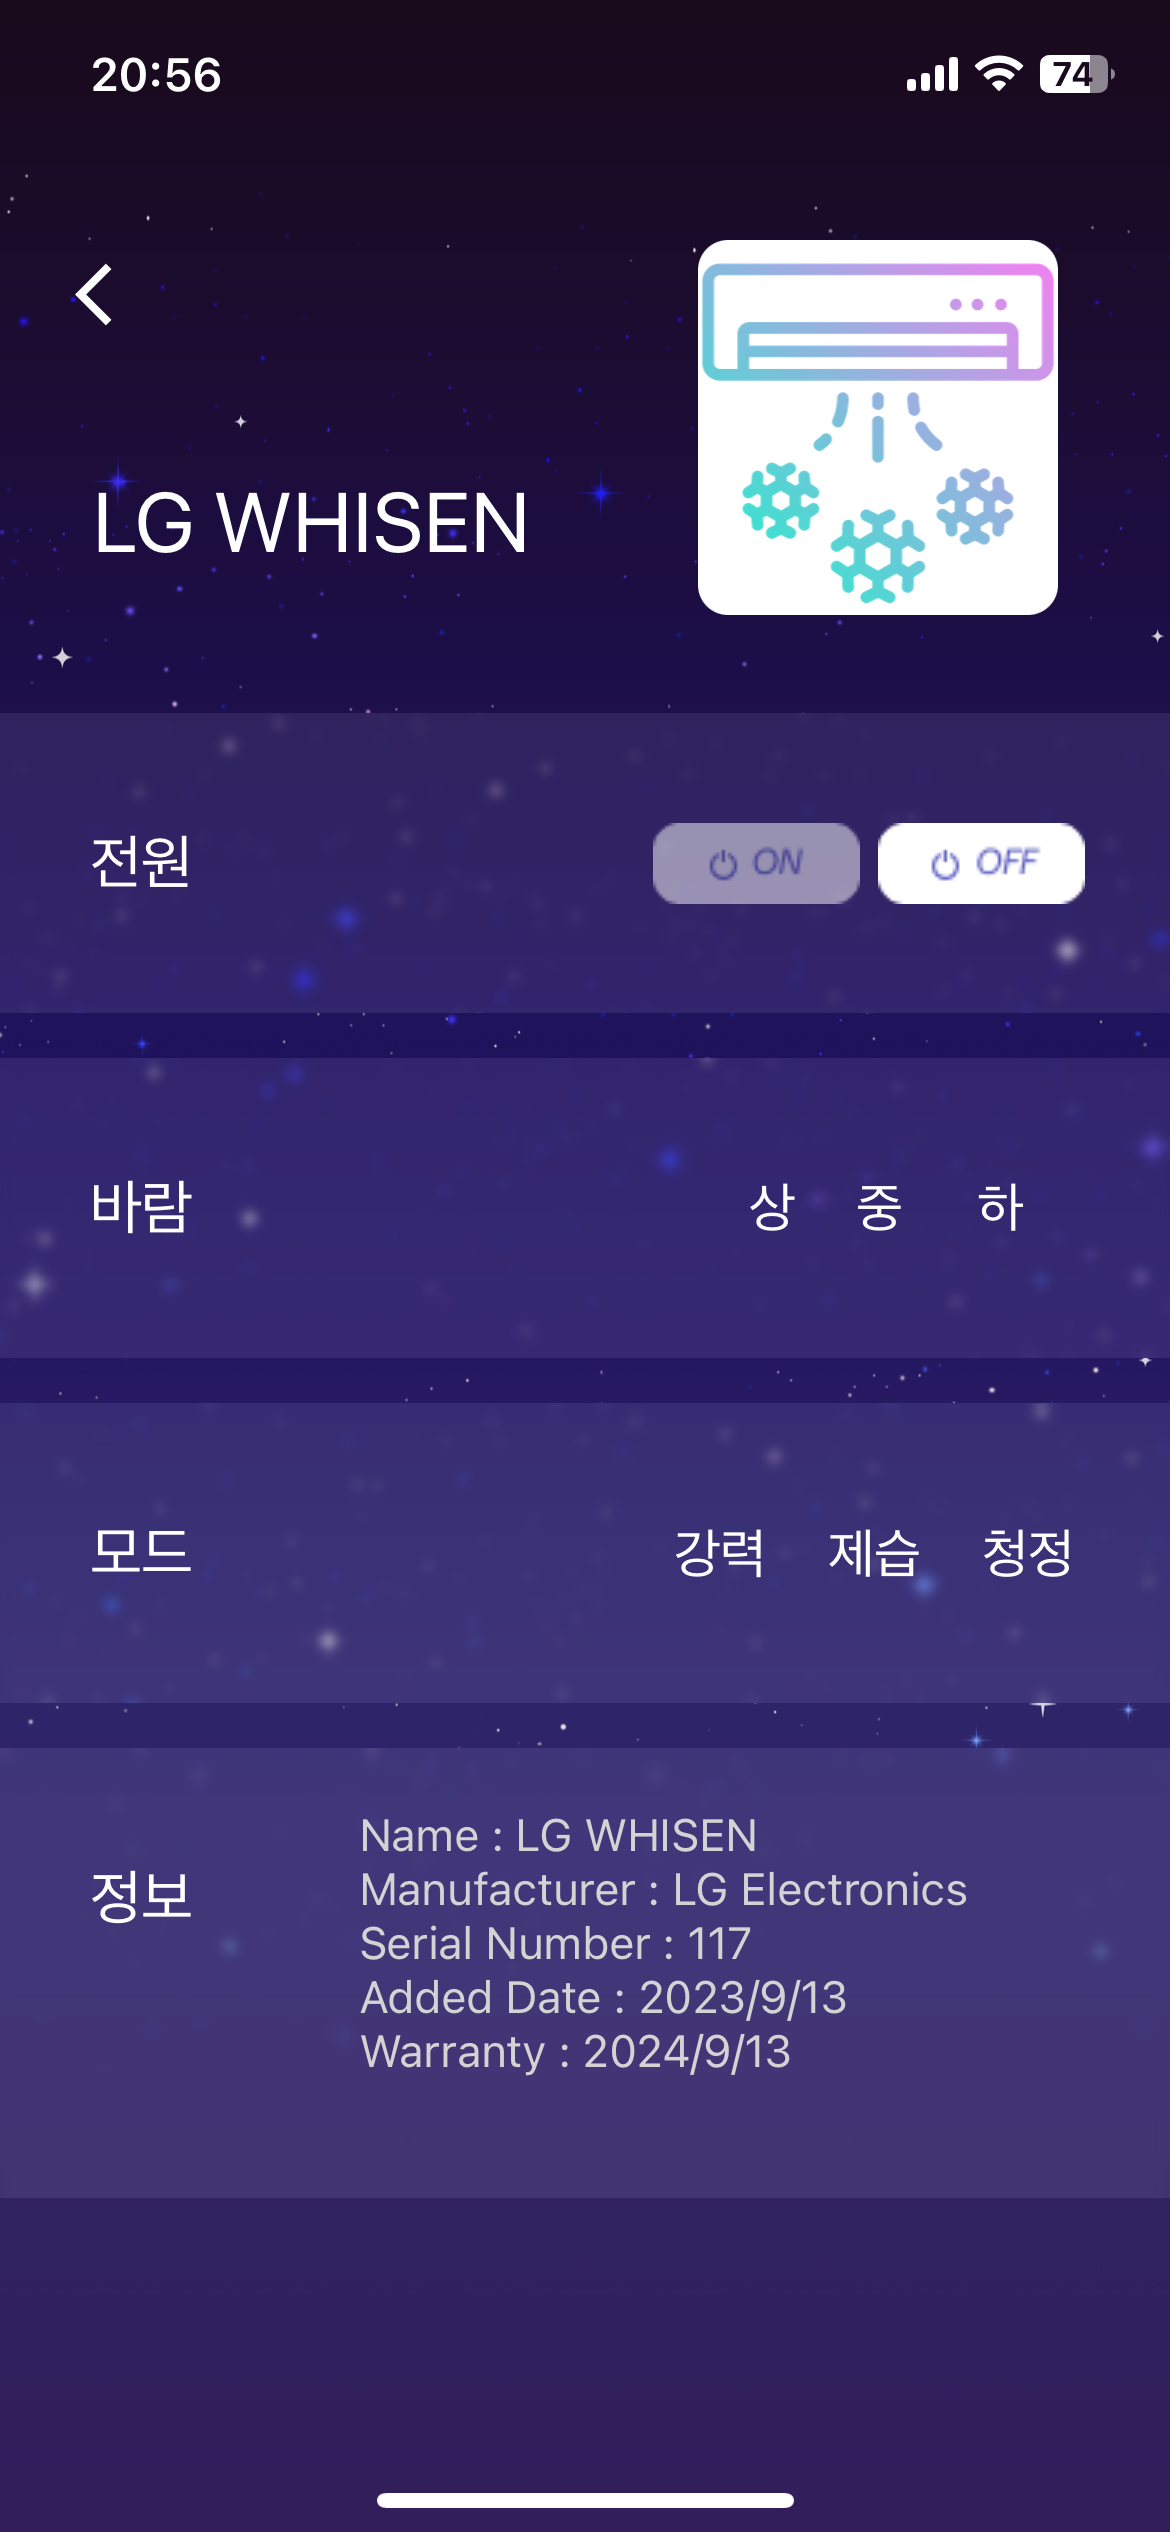
\includegraphics[width=3cm]{Images/screen/elec/8_ELEC_SETTING.PNG}}
            \caption{Appliance Control}
            \label{fig}
        \end{figure}
        For all appliances, you have the on/off function. If it's an air conditioner, you can control temperature, fan speed, energy-saving mode, and reservation functions. If it's an air purifier, you can control fan speed, view particulate matter (PM) levels, and fine particulate matter (PM2.5) levels. If it's a steamer, you can select courses and view the timer. For robot vacuum cleaners, you can choose cleaning modes, select strong, medium, or weak power, and enable quiet mode. Each appliance has its specific and detailed control features.
    \subsection{Game Dashboard}
        \begin{figure}[htbp]
            \centerline{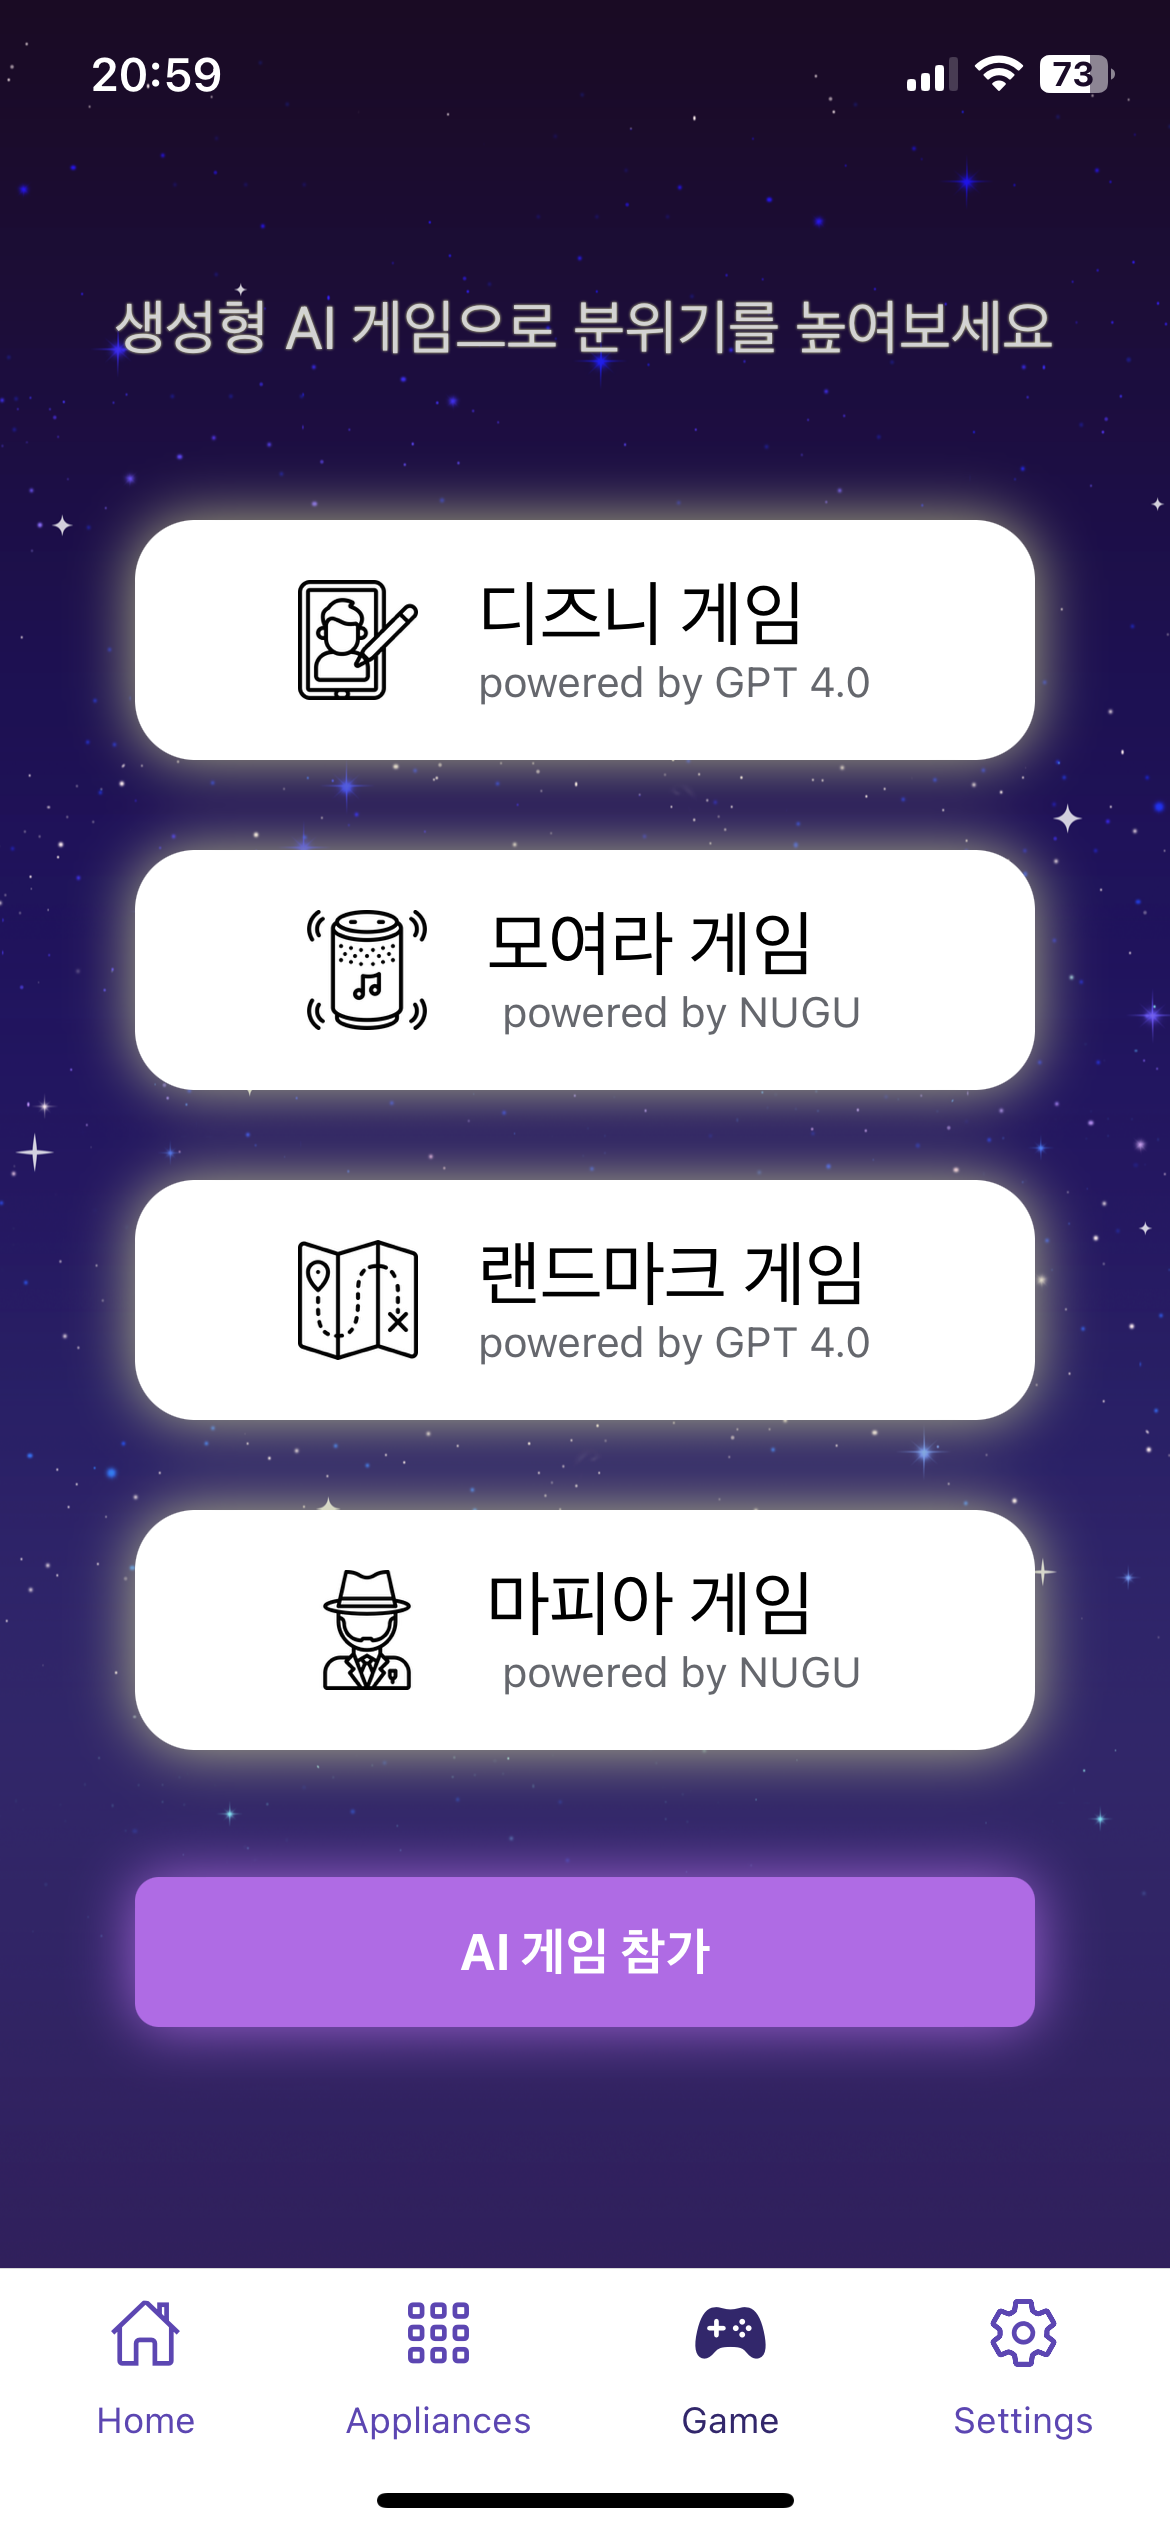
\includegraphics[width=3cm]{Images/screen/game/GAME_LIST.PNG}}
            \caption{Game Dashboard}
            \label{fig}
        \end{figure}
        The game dashboard is the gateway to playing any of the game provided by the application. The main function is to show the list of games available and by pressing on a component of a list, it will activate the game. The details of the games such as name, the logic of the game are all coming from the server, which means that any kind of game can be added anytime on the back-end.\\
        Upon entering the main tab, the data context received is used to display the list of games on the screen. Clicking on a game in the list creates a game room (Game\_Room DB), with the first person to click becoming the game's host. Subsequently, they are connected to the host's screen. (Only one game room can be created within a space.) Clicking the "Join" button allows a user to join a game room currently in progress in the space. Subsequently, they are connected to the participant's screen. The game list received from the server is displayed in a single column on the screen.

    \subsection{Game Host Page}
        \begin{figure}[htbp]
            \centerline{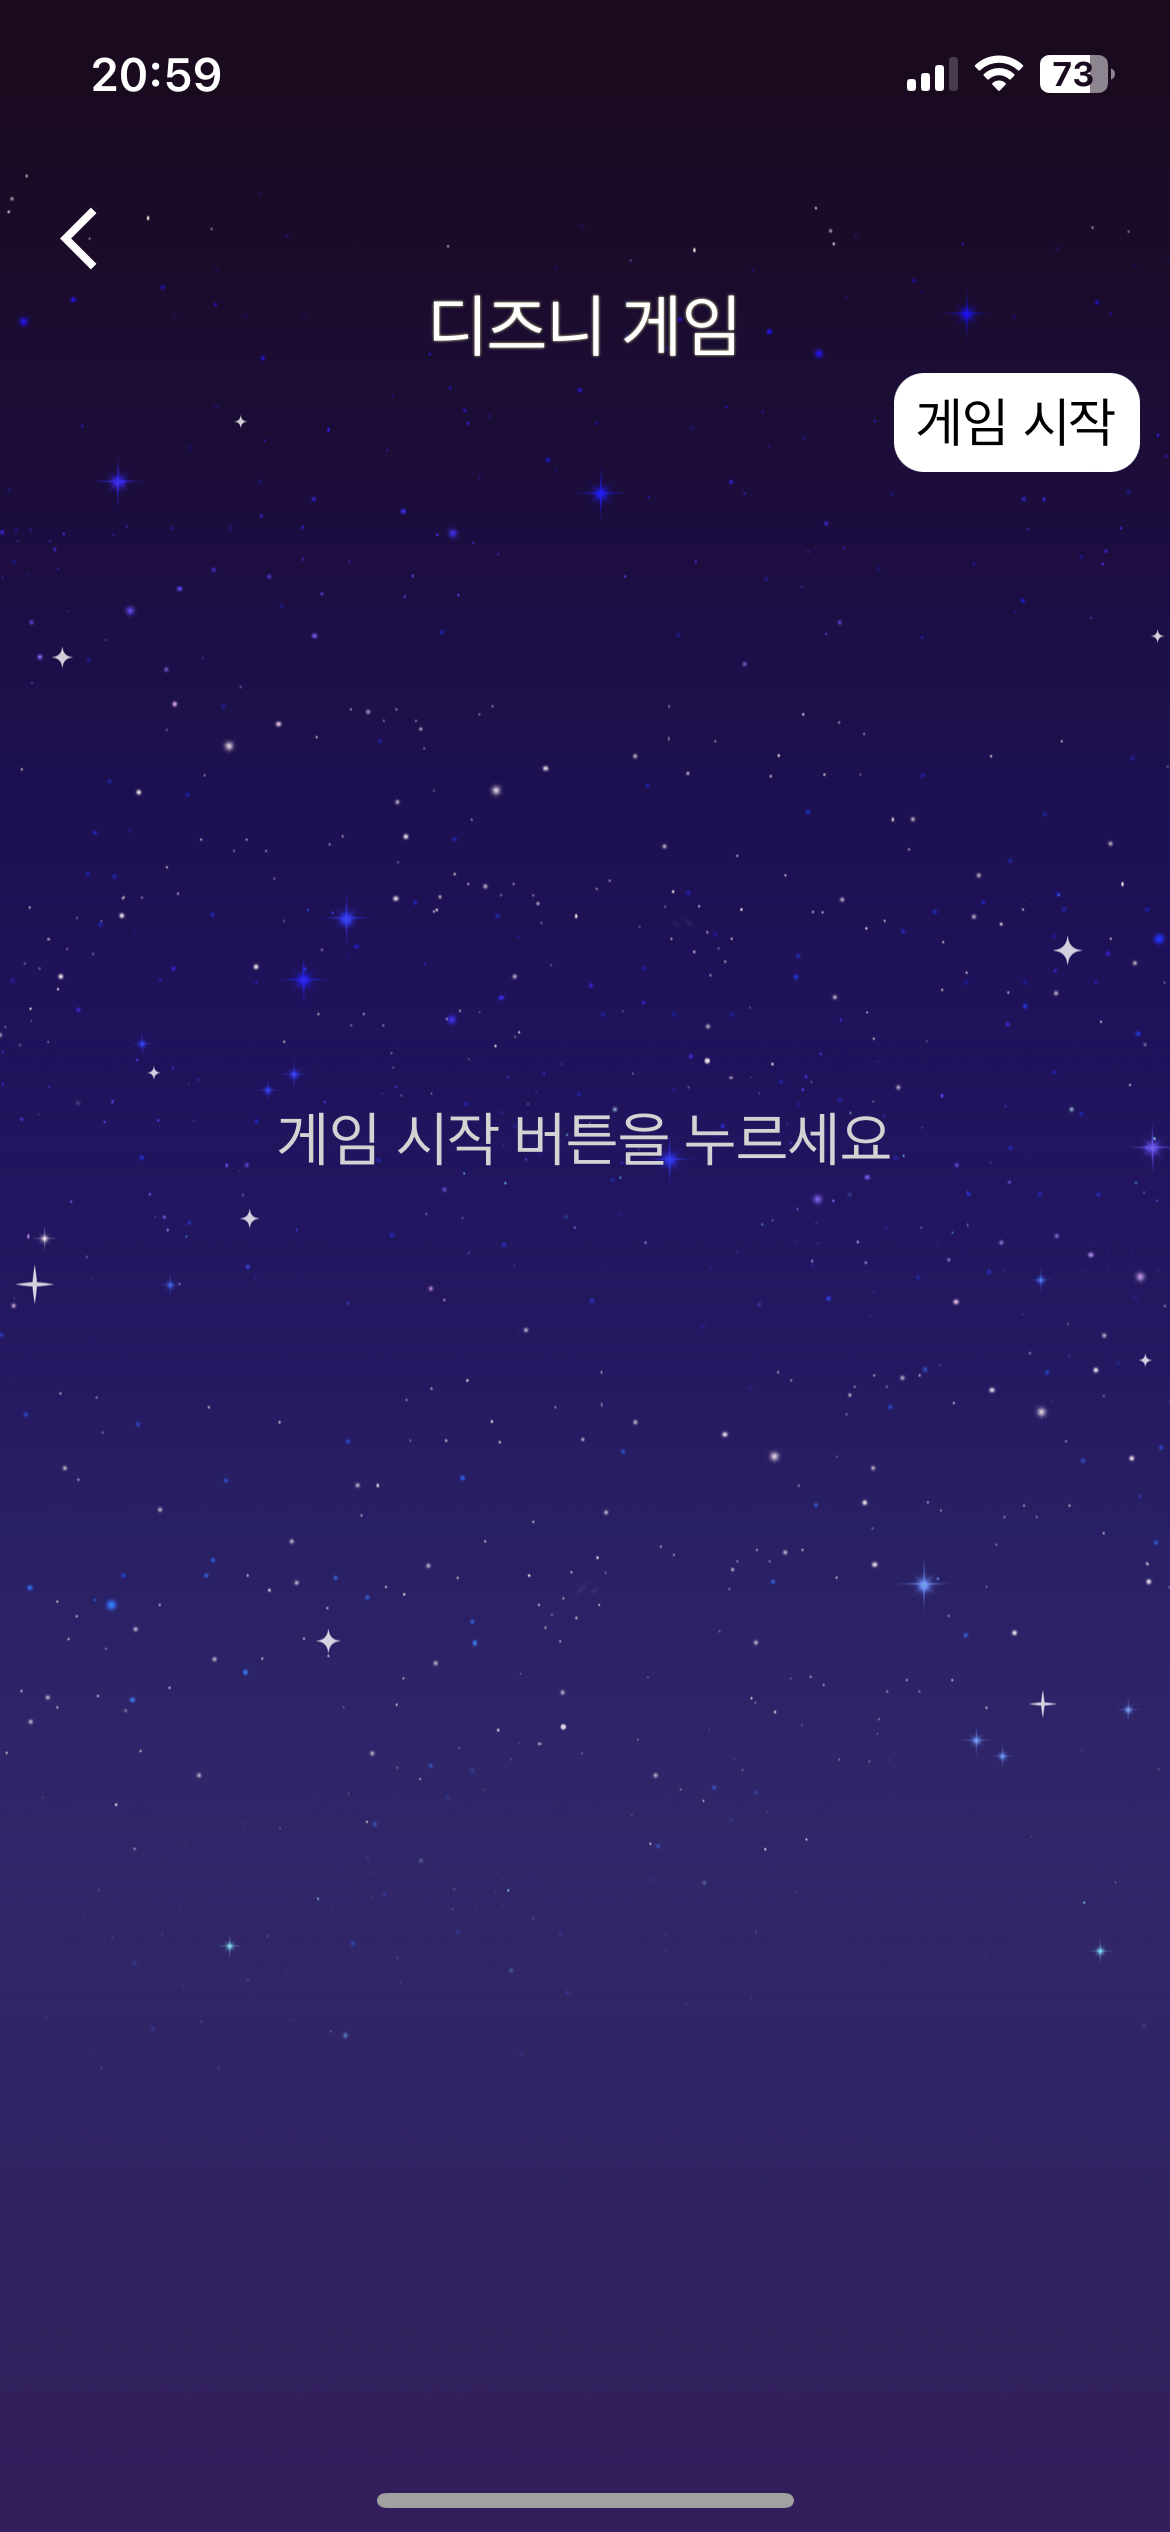
\includegraphics[width=3cm]{Images/screen/game/GAME_STANDBY.PNG}
            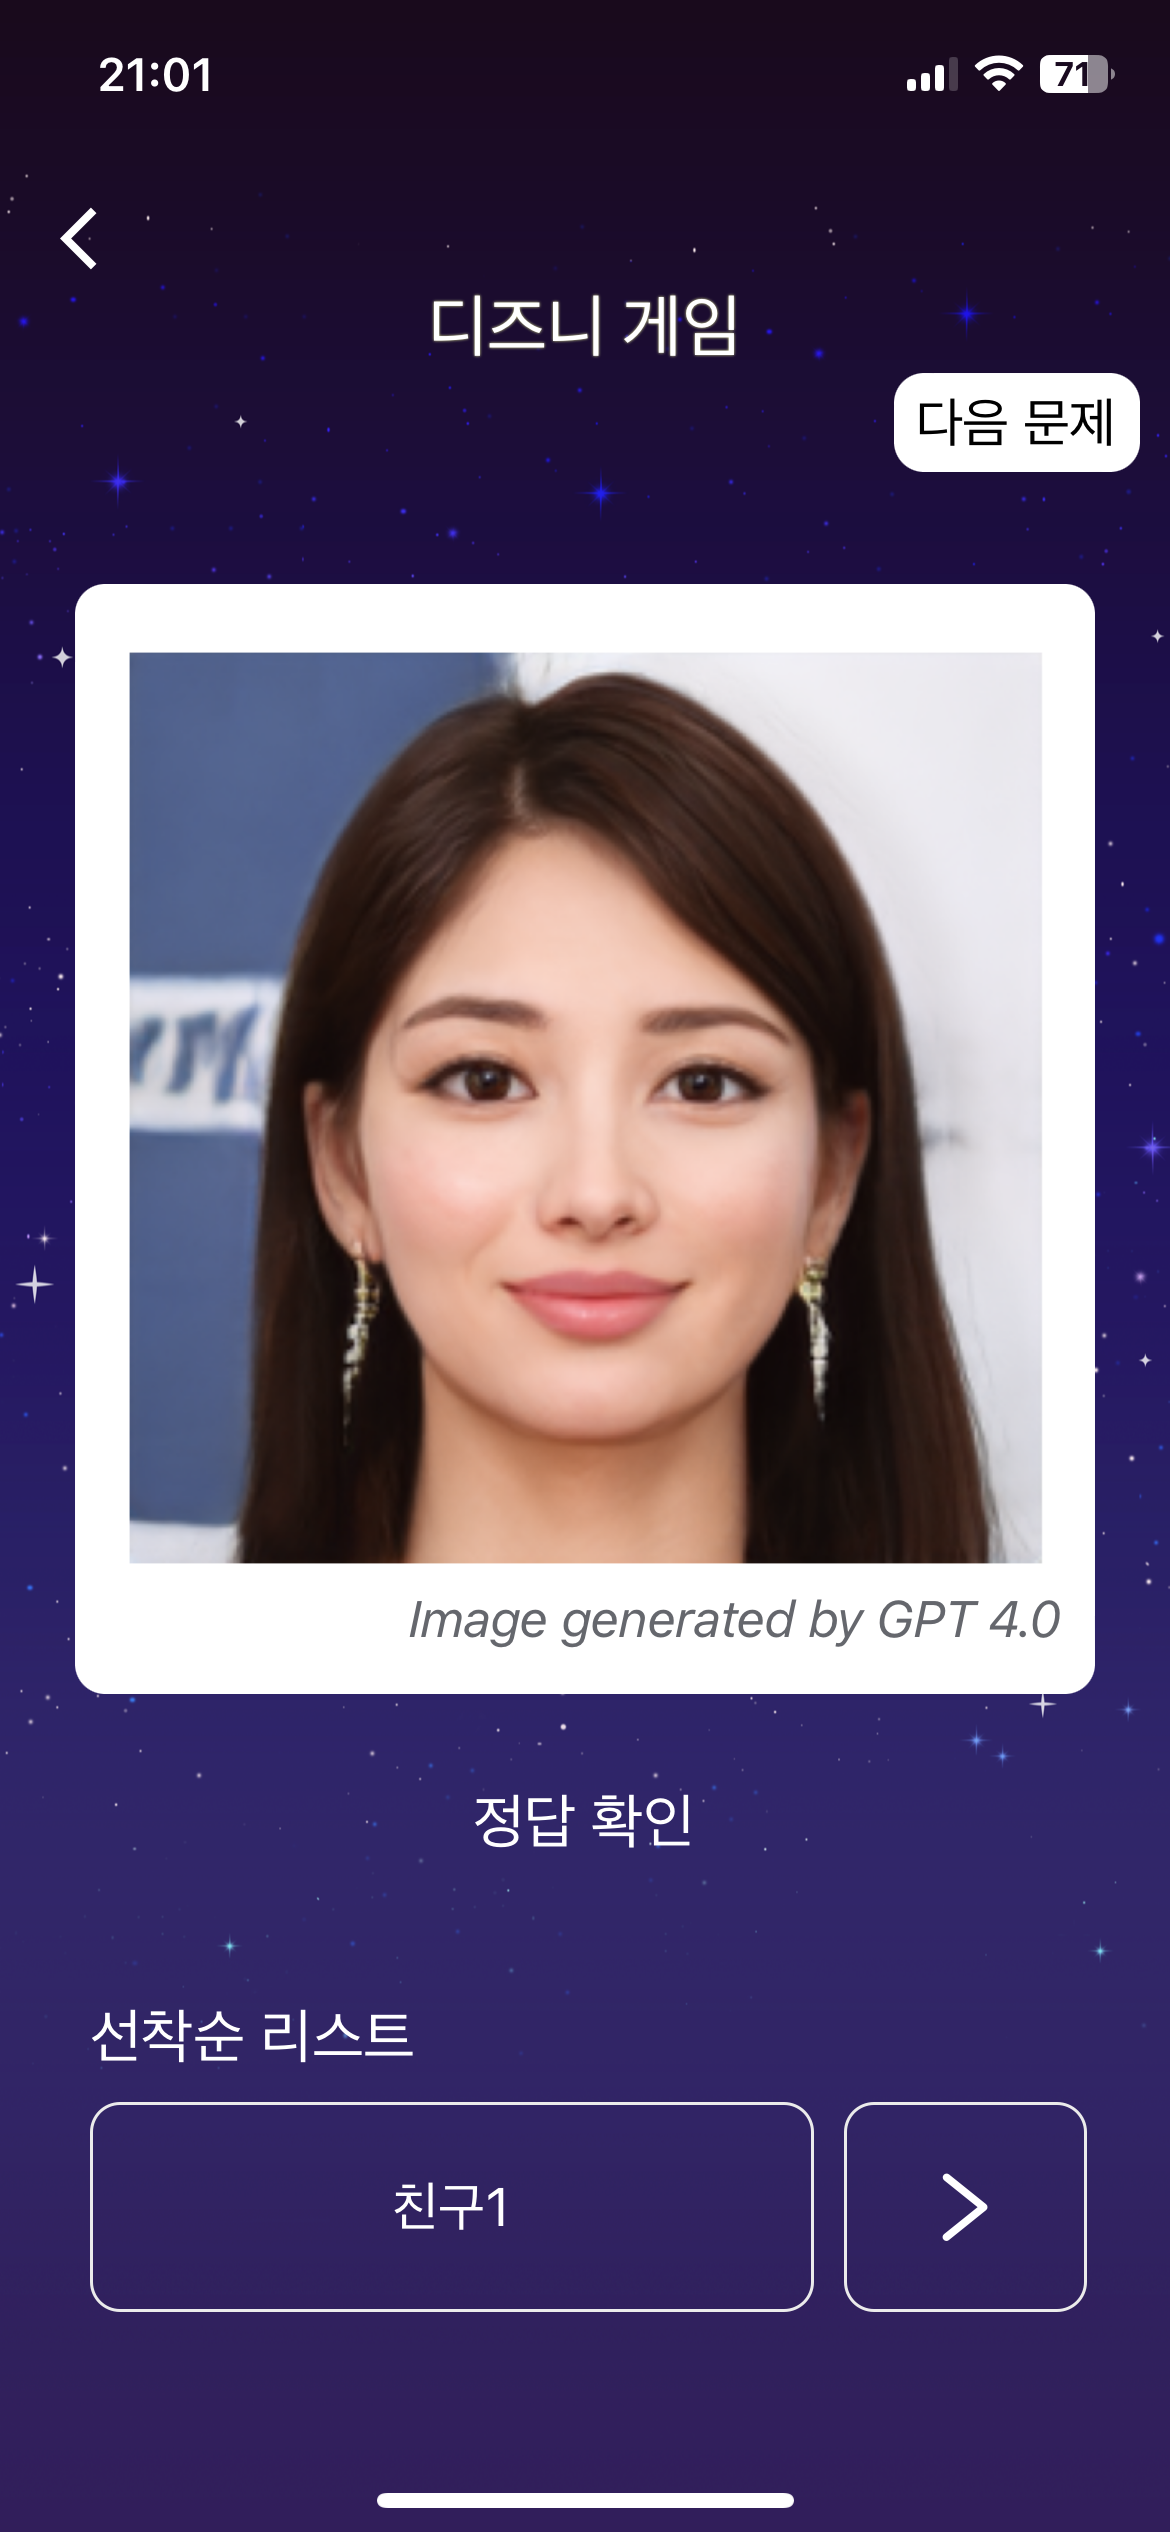
\includegraphics[width=3cm]{Images/screen/game/disney/DISNEY1_HOST.PNG}
            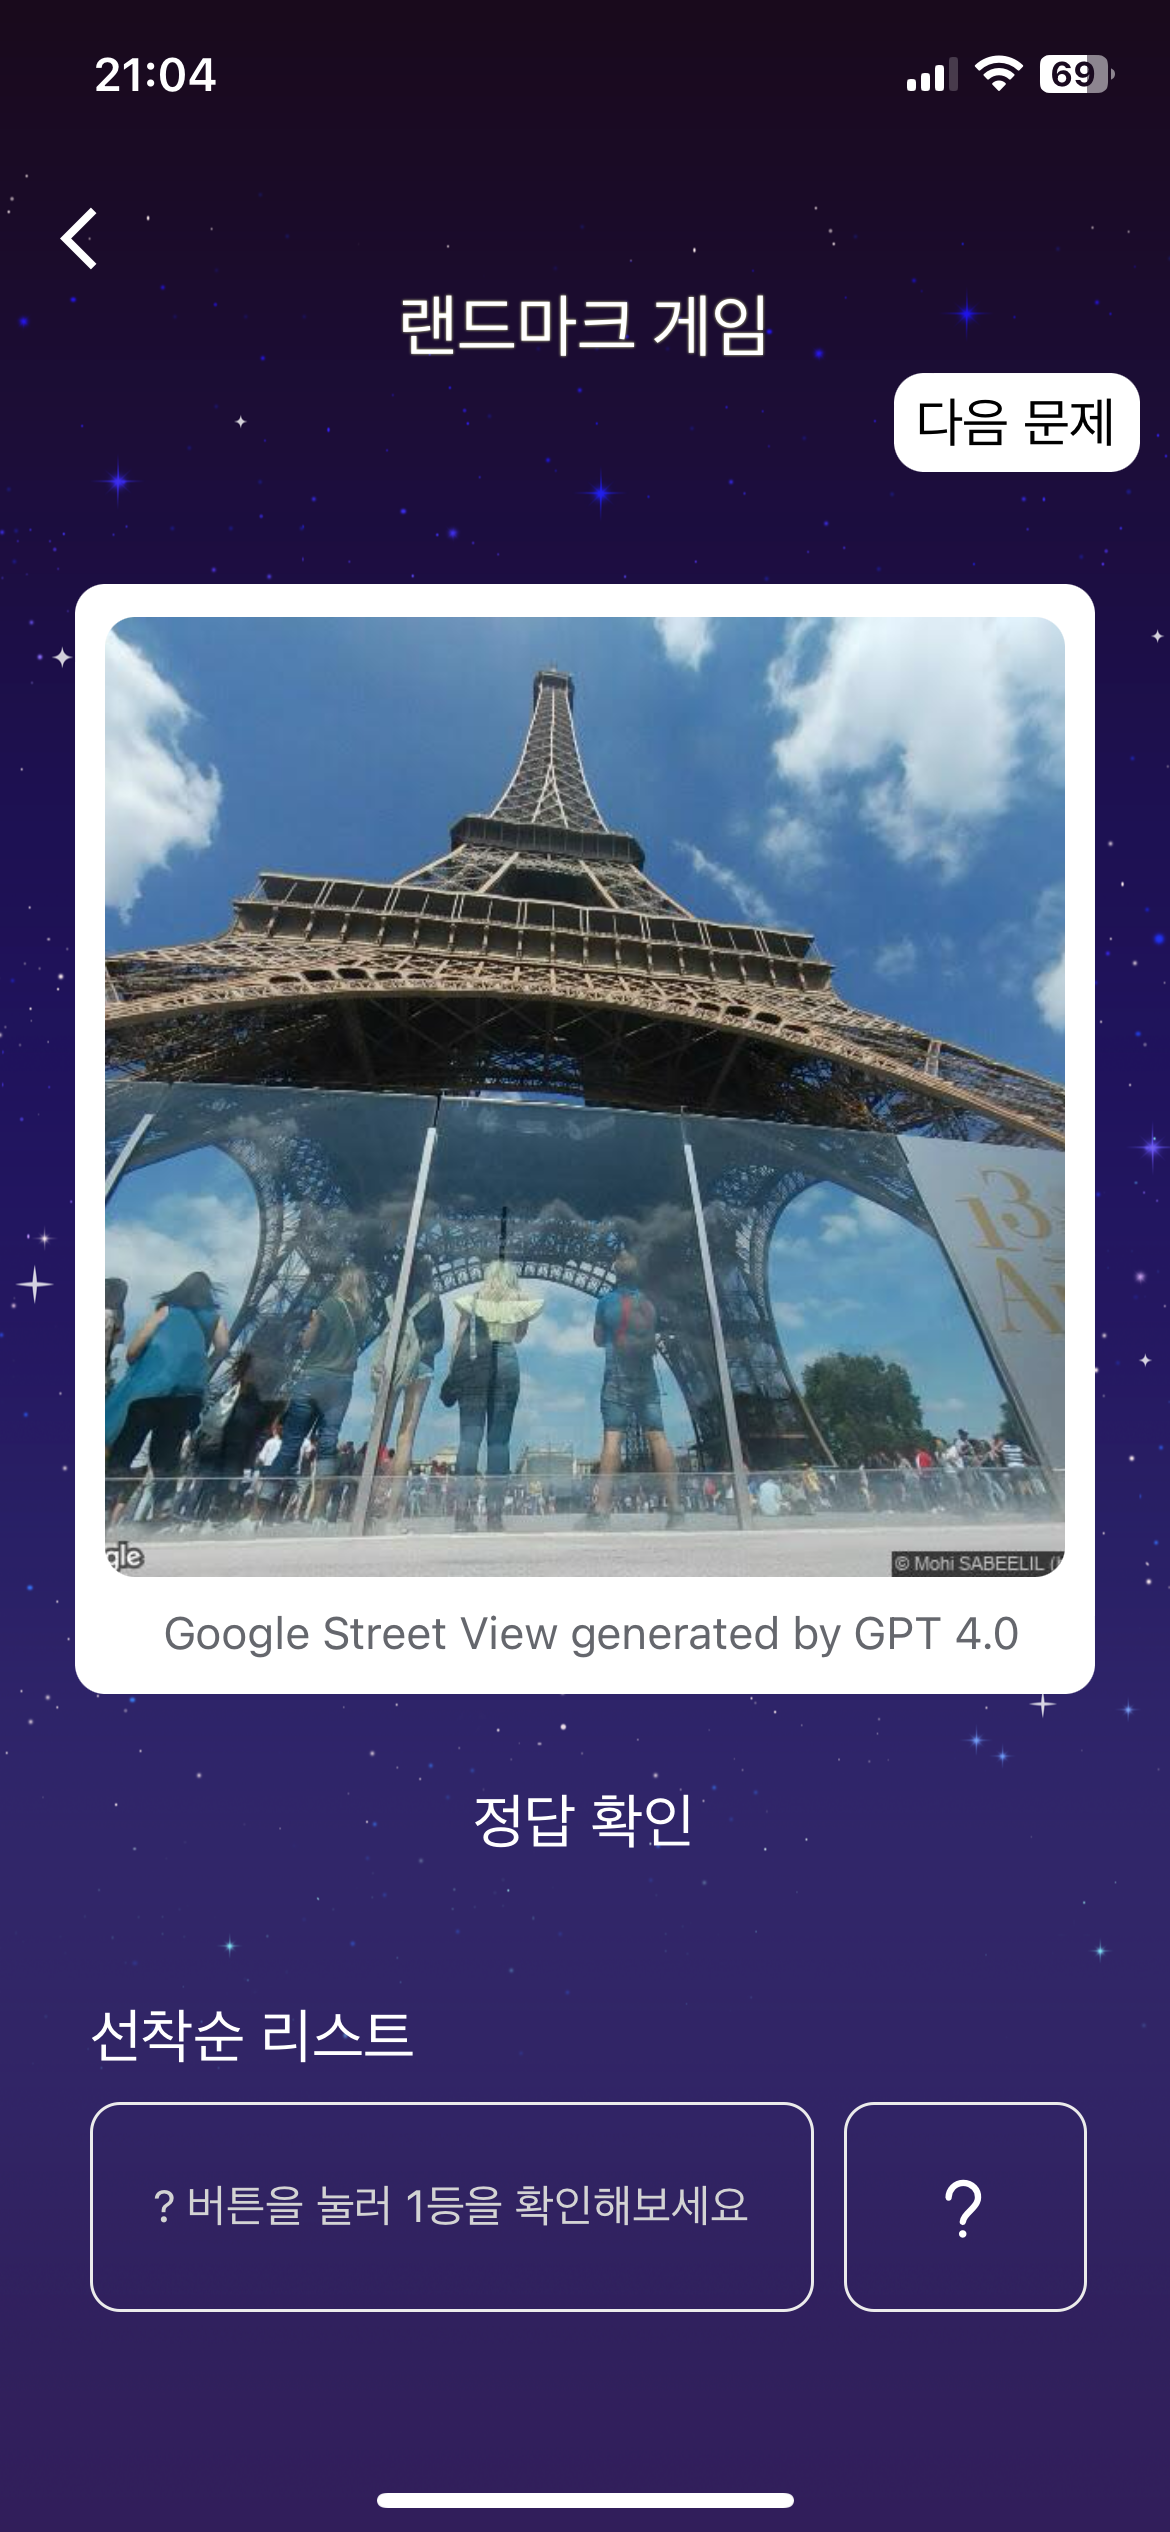
\includegraphics[width=3cm]{Images/screen/game/geo/GEO1_HOST.PNG}}
            \caption{Game Host}
            \label{fig}
        \end{figure}
        The game host page is a page for the first person to press a game on the game list. By being the first person pressing, it automatically makes them the host of the game. The host’s page consists of all information needed to run the game such as game question, game answer, go to next quiz, end game and a serial list of users based on the speed of pressing the answering button. The host can give user chances to answer according to the list of users and verify if the player has got the answer right. If the answer is correct or nobody got the answer or any situation that regards to move on, the host can press the next game button.\\
        Upon entering the screen, a WebSocket connection is established, and a request with messageType = ENTER is sent. When the "Next Question" button is pressed, the Flask server fetches the question for the selected game, sends it over WebSocket to display it for all participants, and sends a request with messageType = NEXT. When the "Reveal Answer" button is pressed, the answer to the received question is sent over WebSocket to display it for all participants, and a request with messageType = ANSWER is sent. At the bottom of the screen, the nickname of the participant at the top of the first-come, first-served list is displayed. Clicking the "Next" button removes the next person from the list.\\
        The name of the selected game is displayed in the top left corner of the screen, while the "End Game" and "Next Question" buttons are positioned in the top right corner. The game screen may vary depending on the type of game, with images displayed for games that require them and a default image for games that do not. At the bottom of the screen, a list of participants in the game, organized by arrival order, is displayed.

    \subsection{Game Participant Page}
        \begin{figure}[htbp]
            \centerline{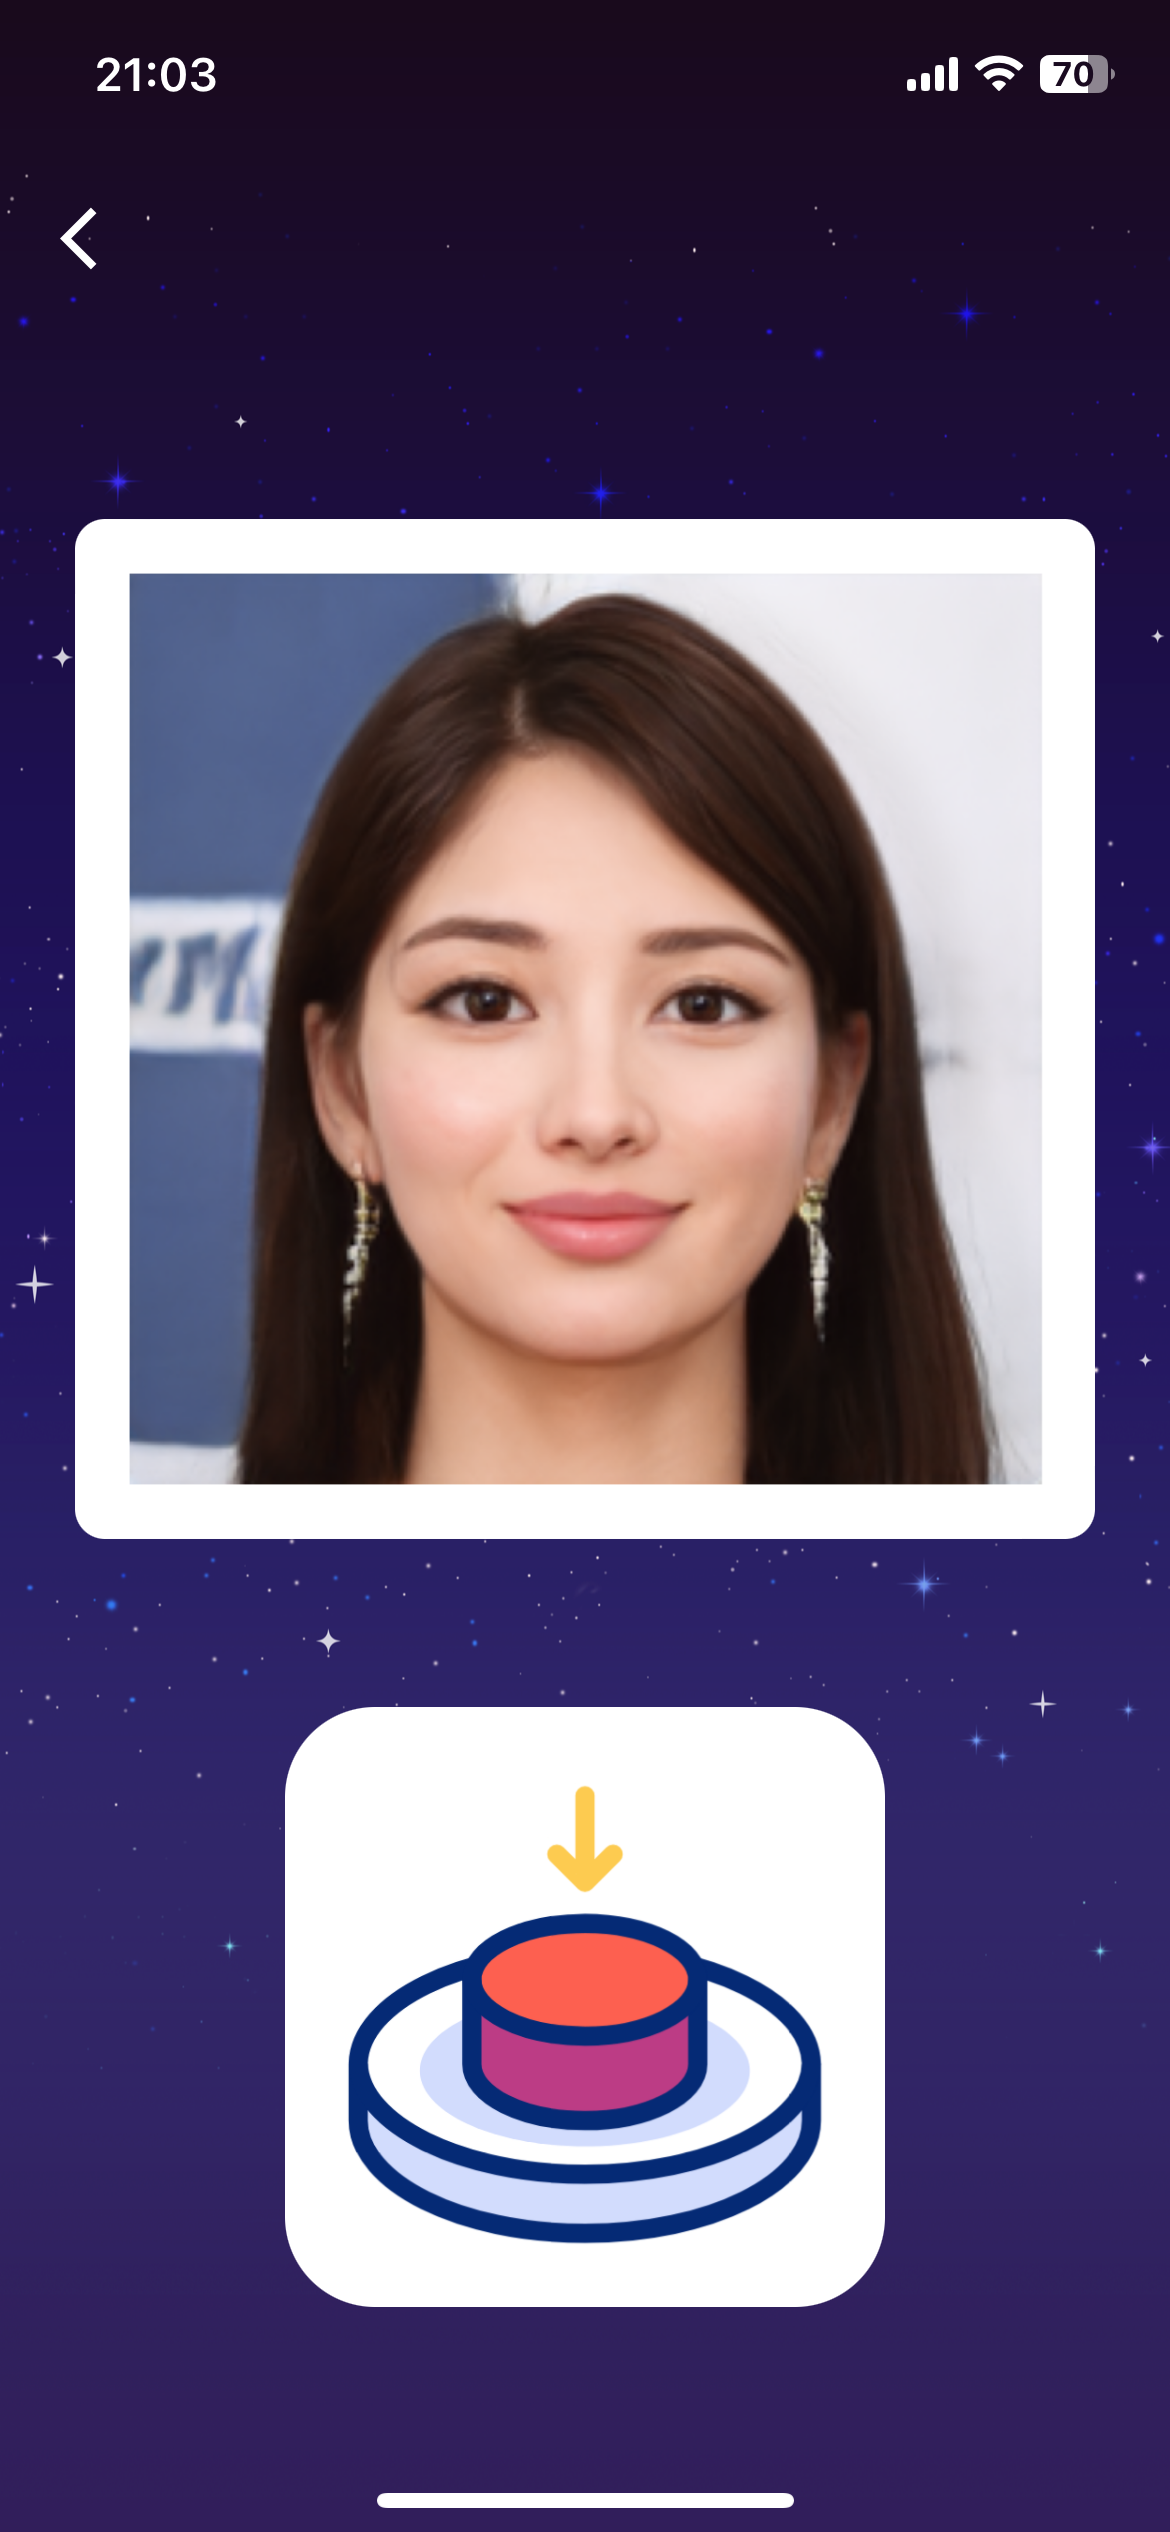
\includegraphics[width=3cm]{Images/screen/game/disney/DISNEY1_PLAYER.PNG}
            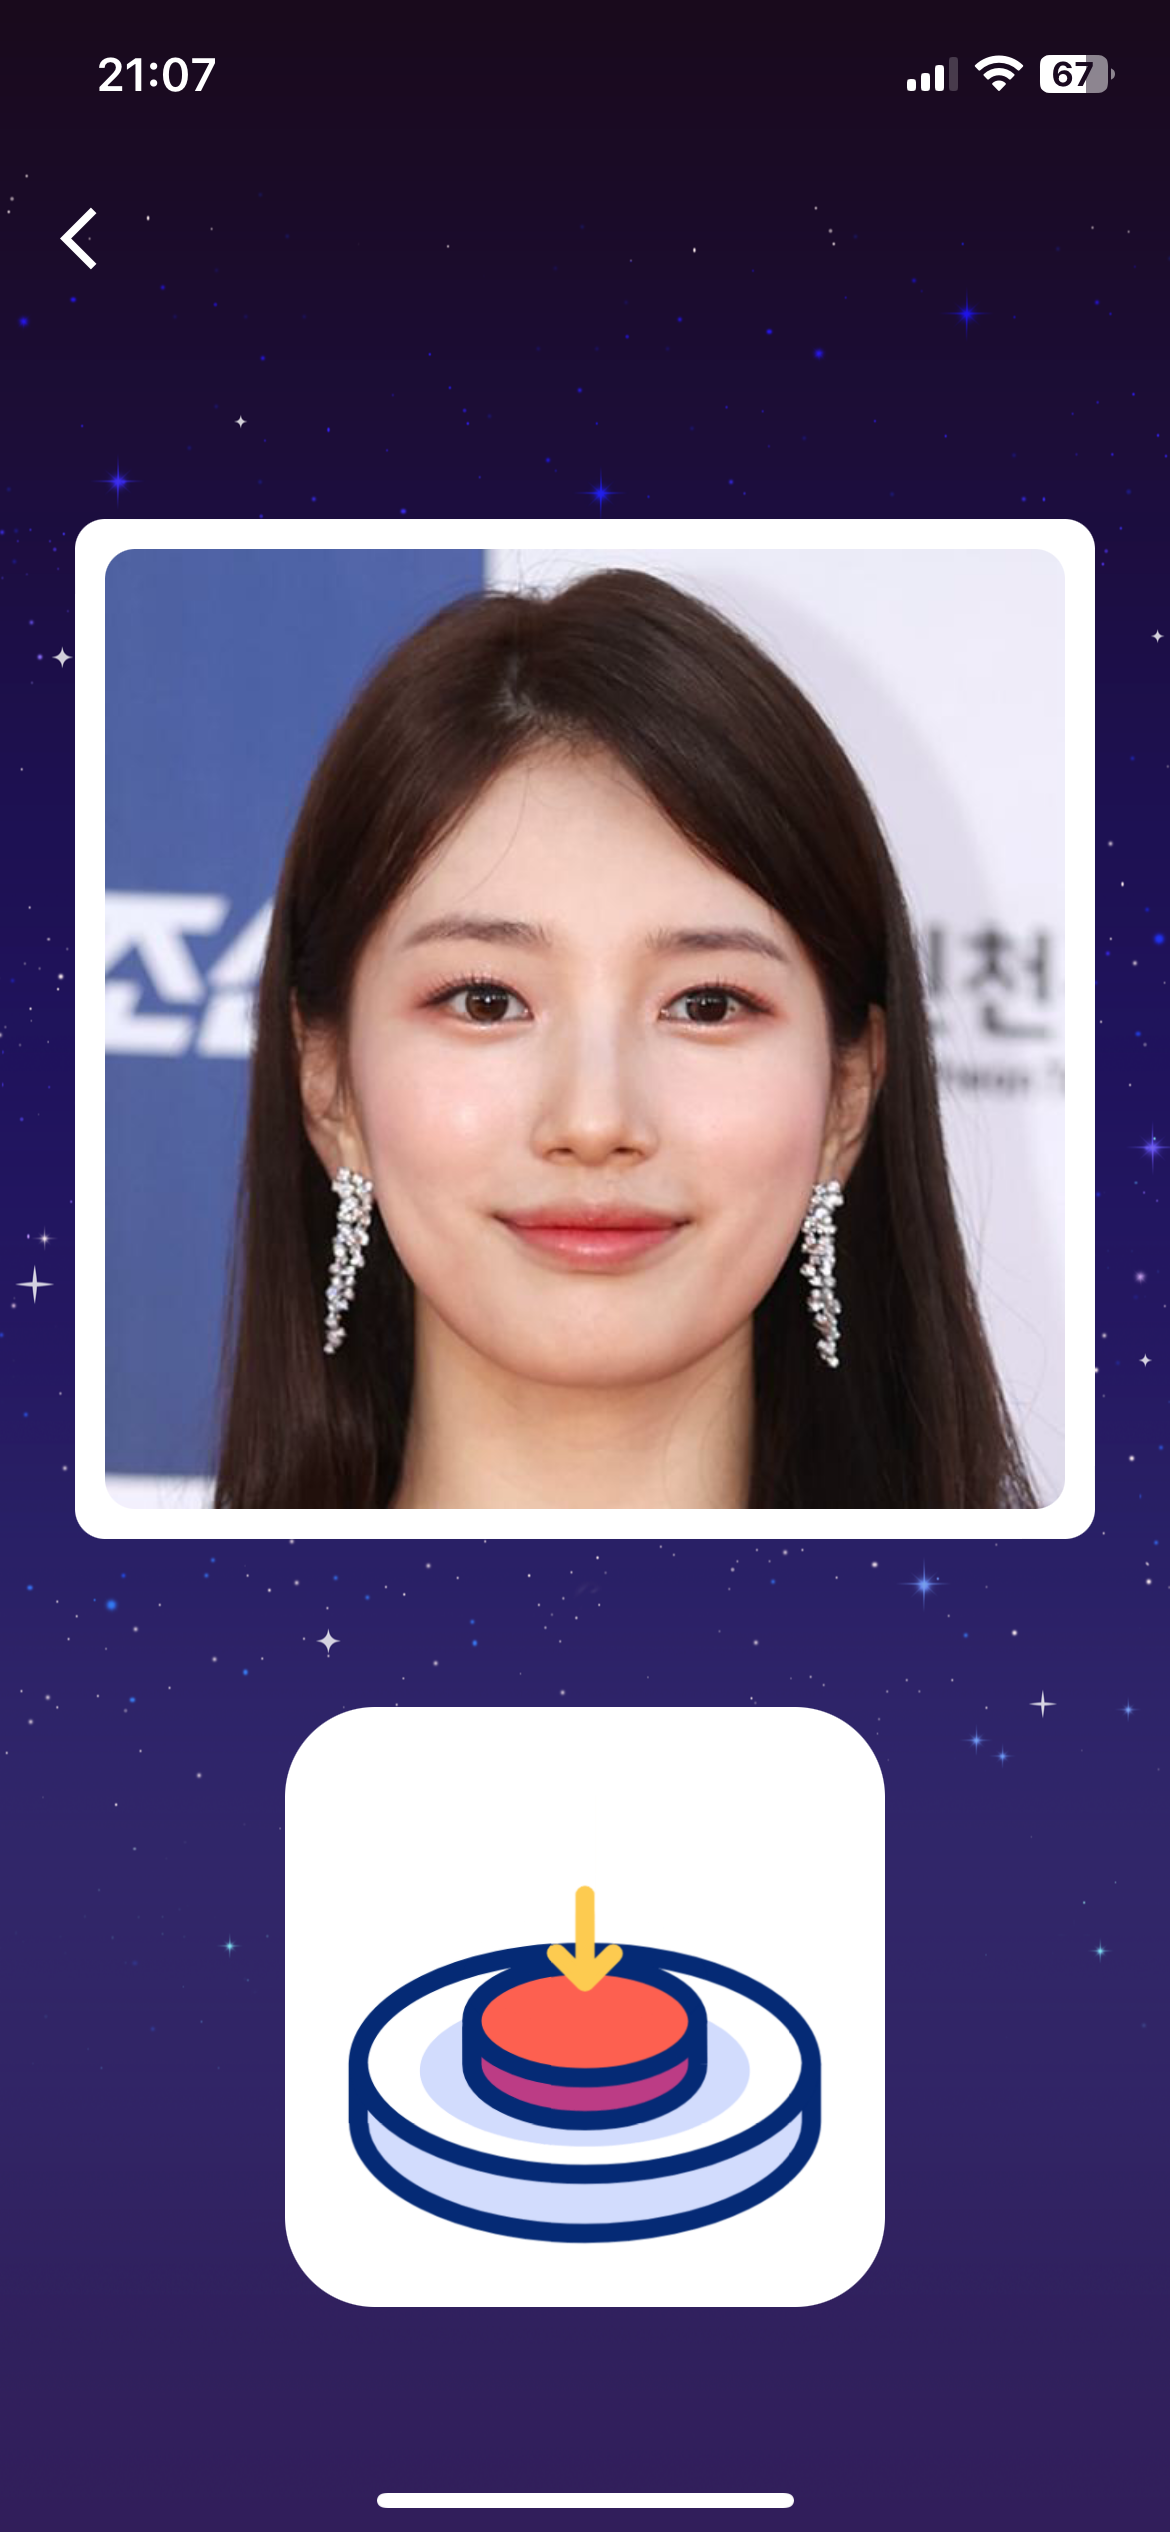
\includegraphics[width=3cm]{Images/screen/game/disney/DISNEY1_PLAYER_ANSWER.PNG}
            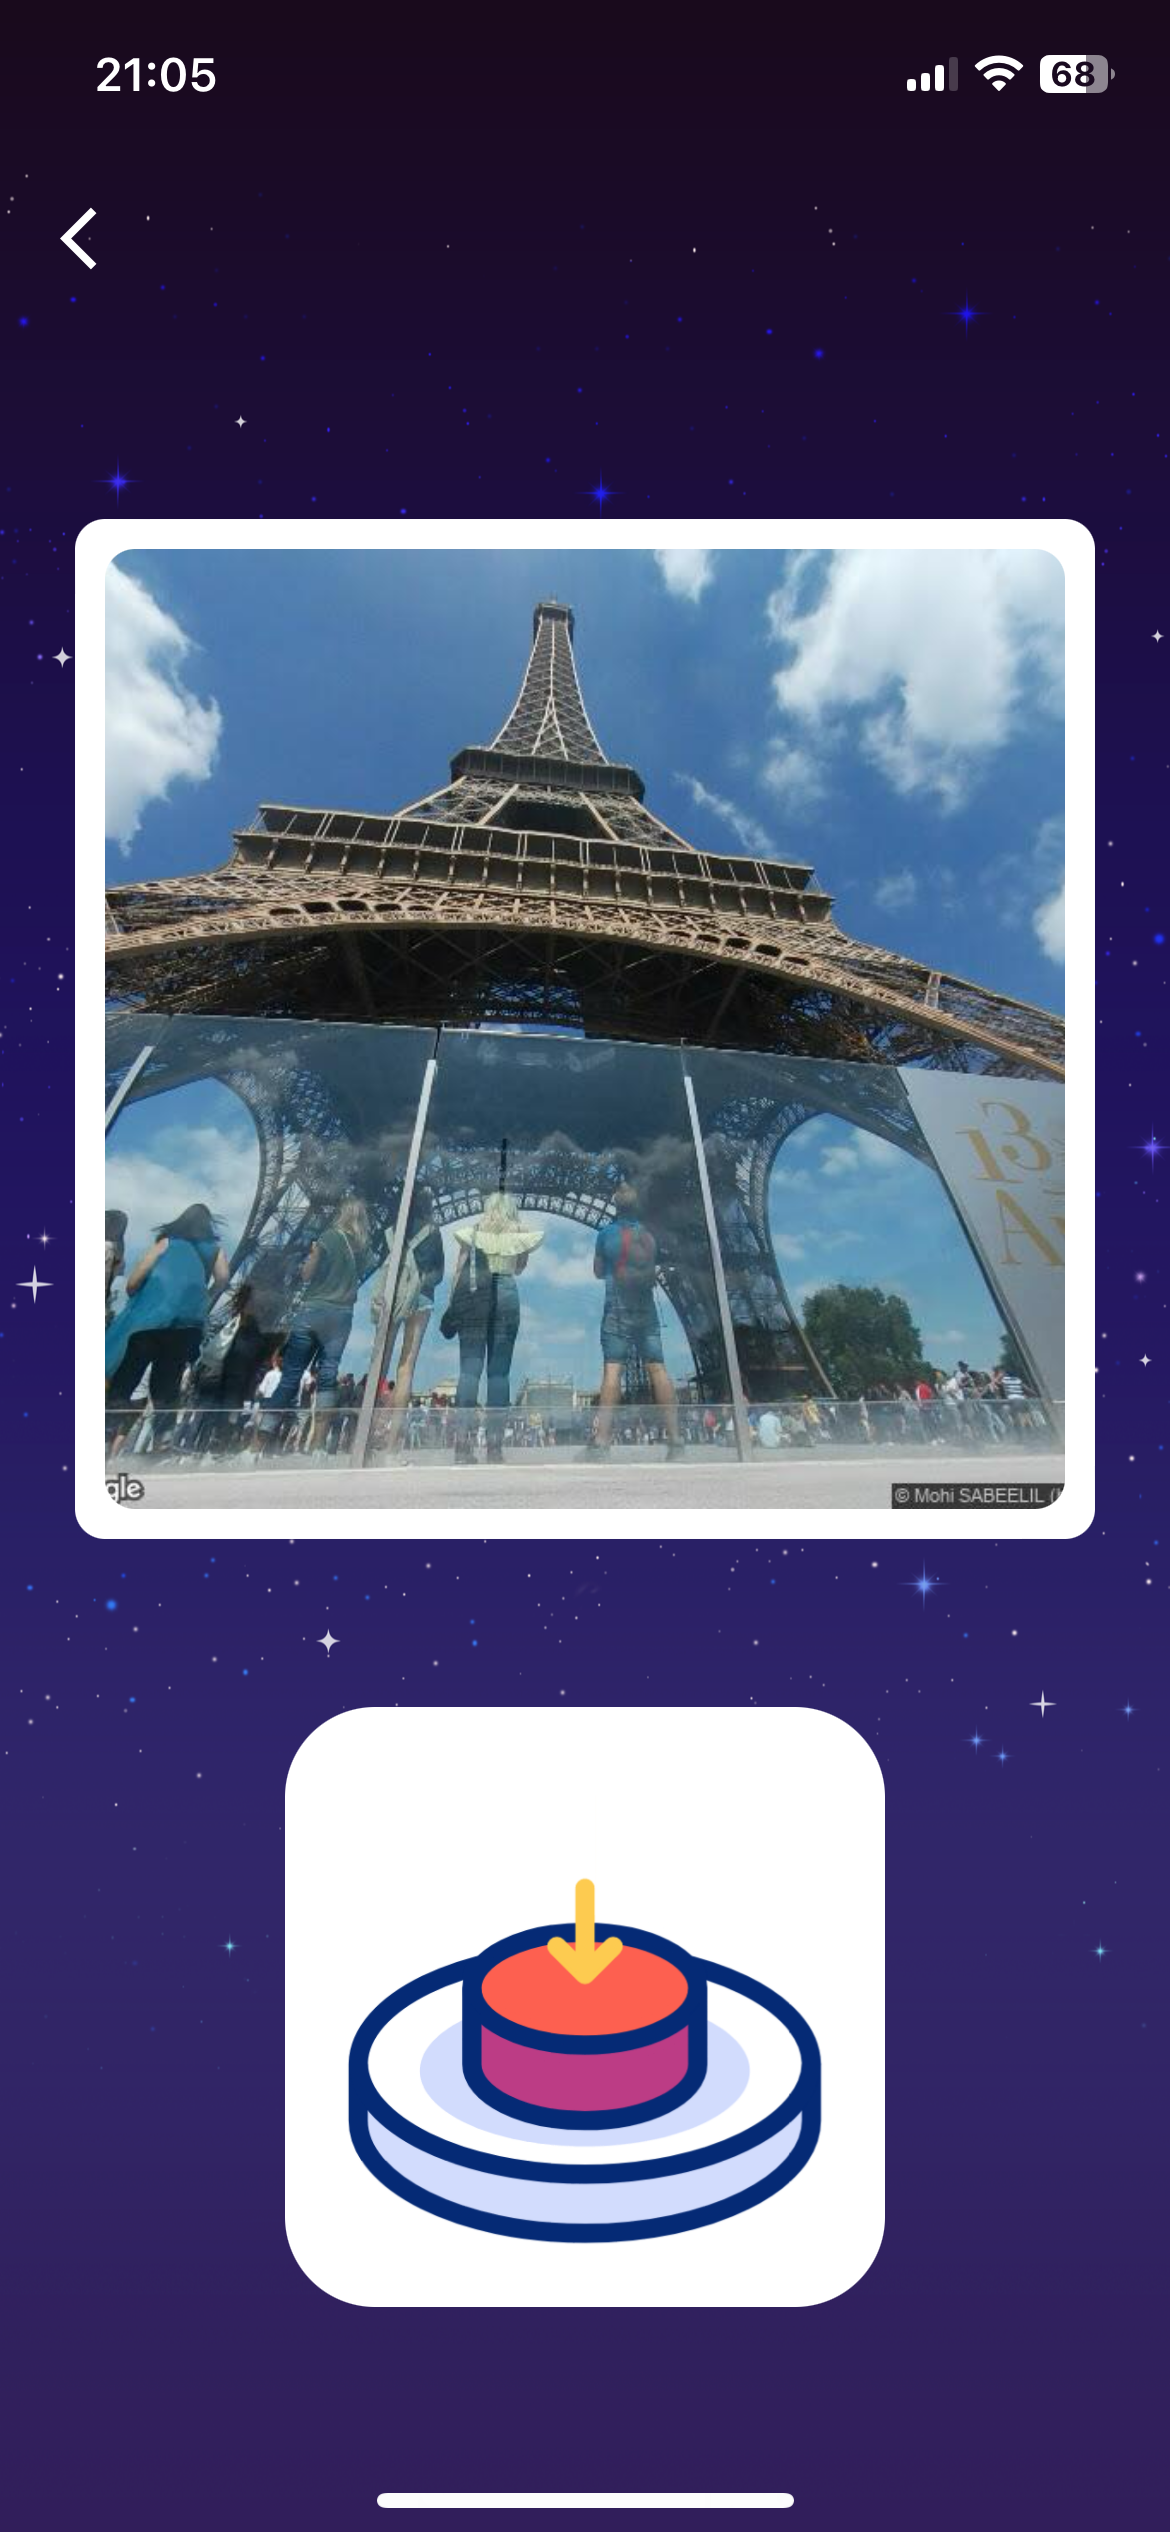
\includegraphics[width=3cm]{Images/screen/game/geo/GEO1_PLAYER.PNG}}
            \caption{Game Participant}
            \label{fig}
        \end{figure}
        Game participant page is for users that are actually playing the game. The same page is displayed to all users. The main functions provided are to see what the question or quiz is, and a button that gives you the chance to answer these questions. \\
        The screen for participants is similar to the game host page but lacks the "End Game" and "Next Question" buttons. When participants press a button, they are added to the list in the order in which they respond. \\
    	Upon entering the screen, a WebSocket connection is established, and a message with messageType = ENTER is sent. When the game host displays a question, all participants automatically receive a request and see the question. Pressing the "Answer" button adds the participant to the list in the Game\_Room DB in a first-come, first-served manner.

    \subsection{AI Guessing Game}
        \begin{figure}[htbp]
            \centerline{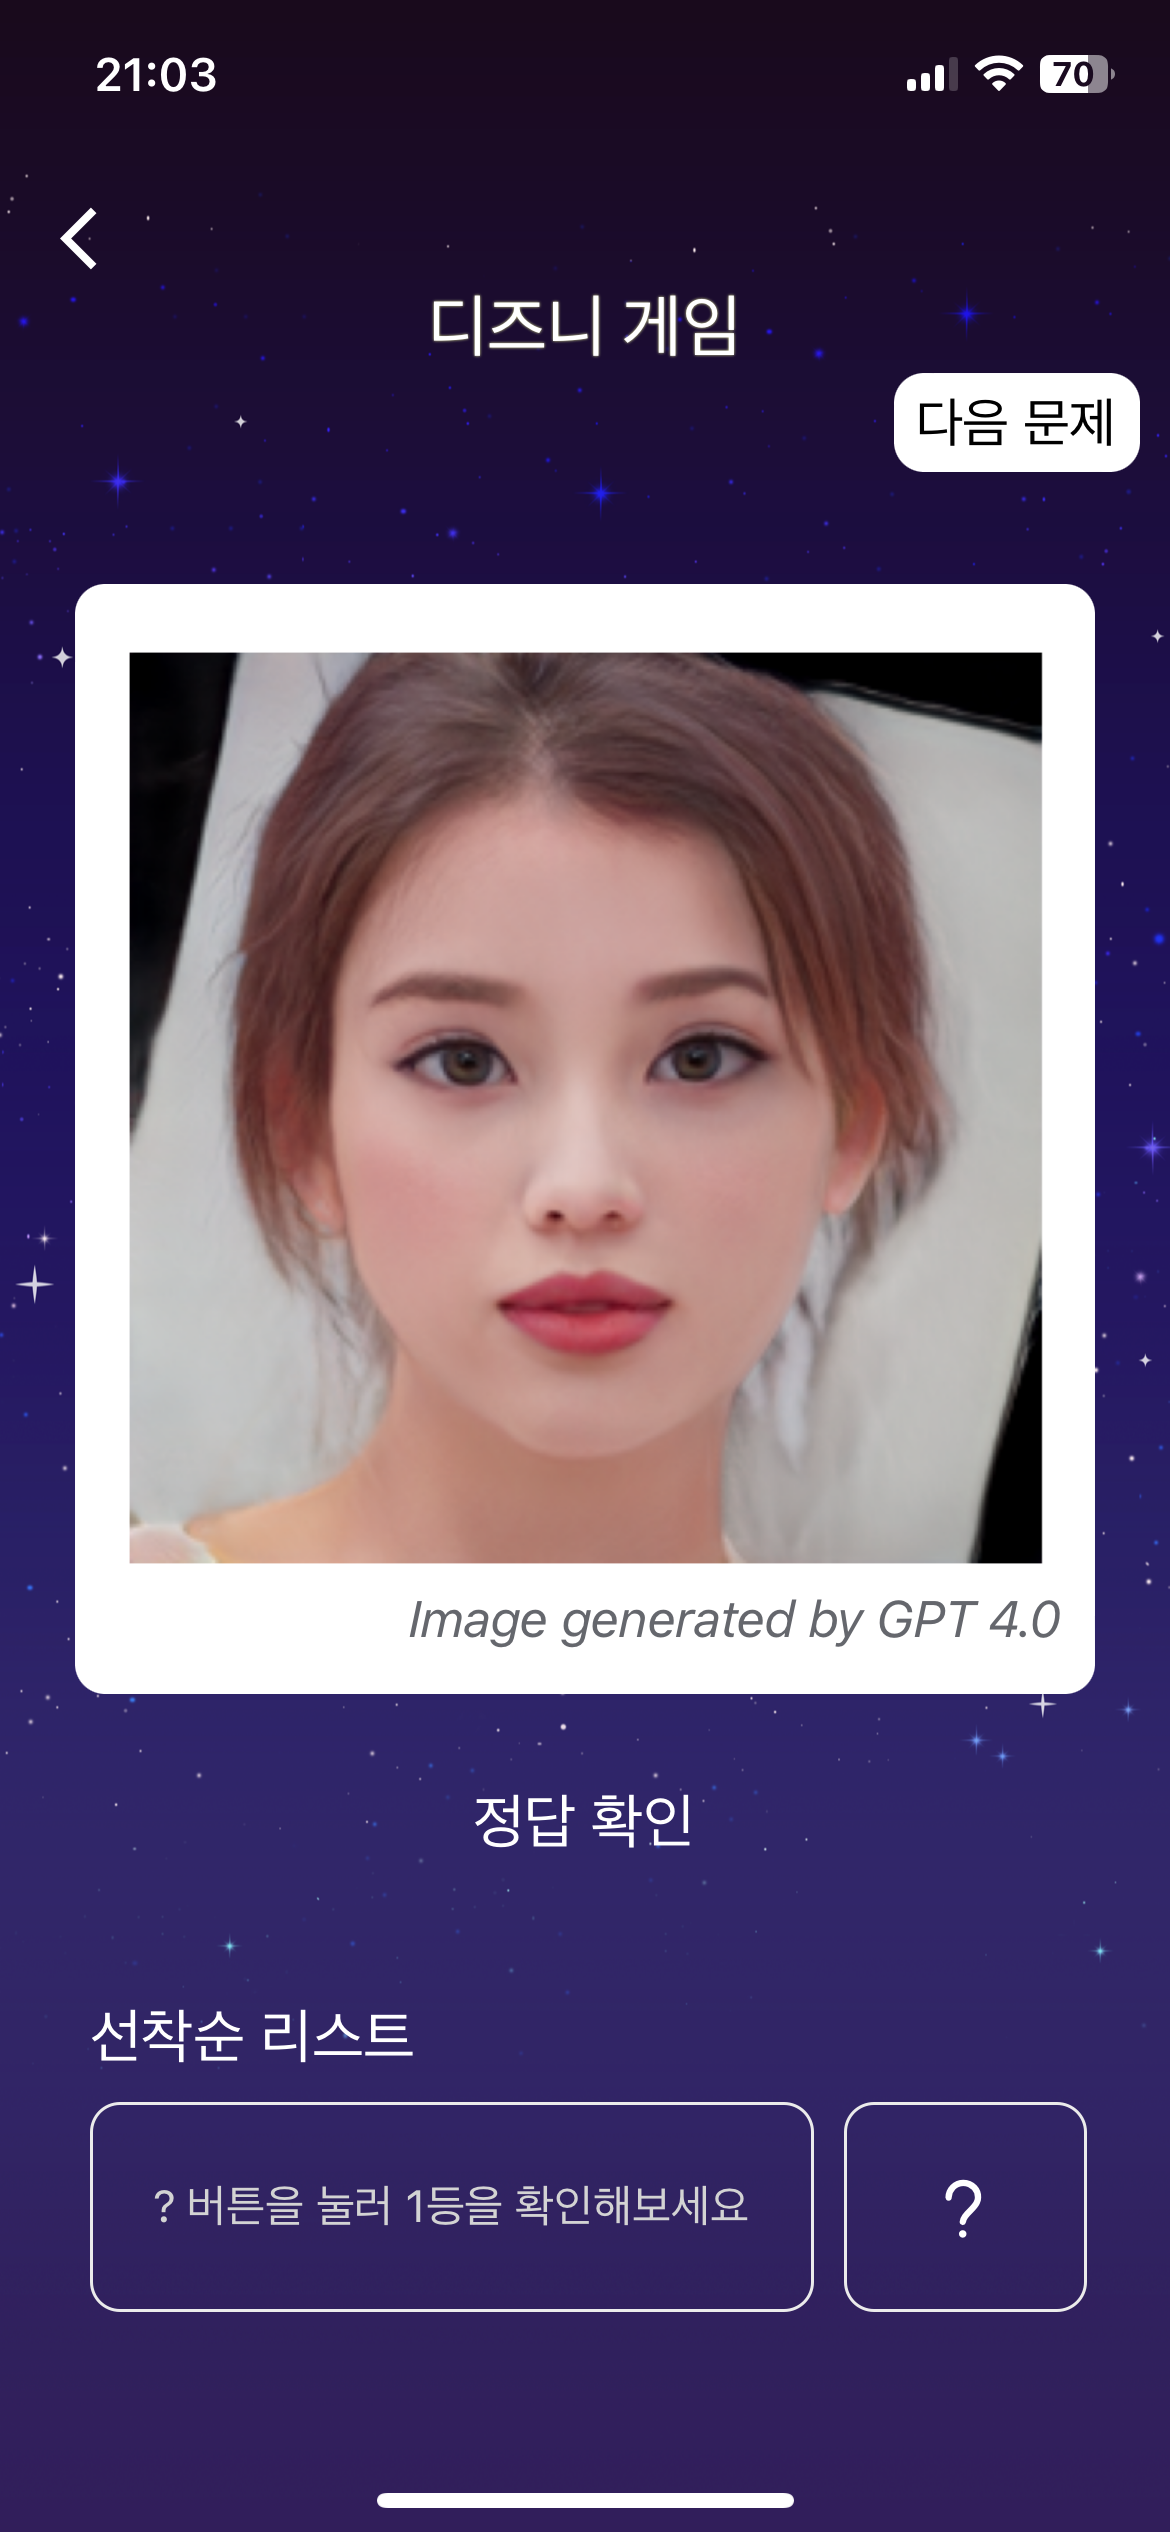
\includegraphics[width=3cm]{Images/screen/game/disney/DISNEY2_HOST.PNG}
            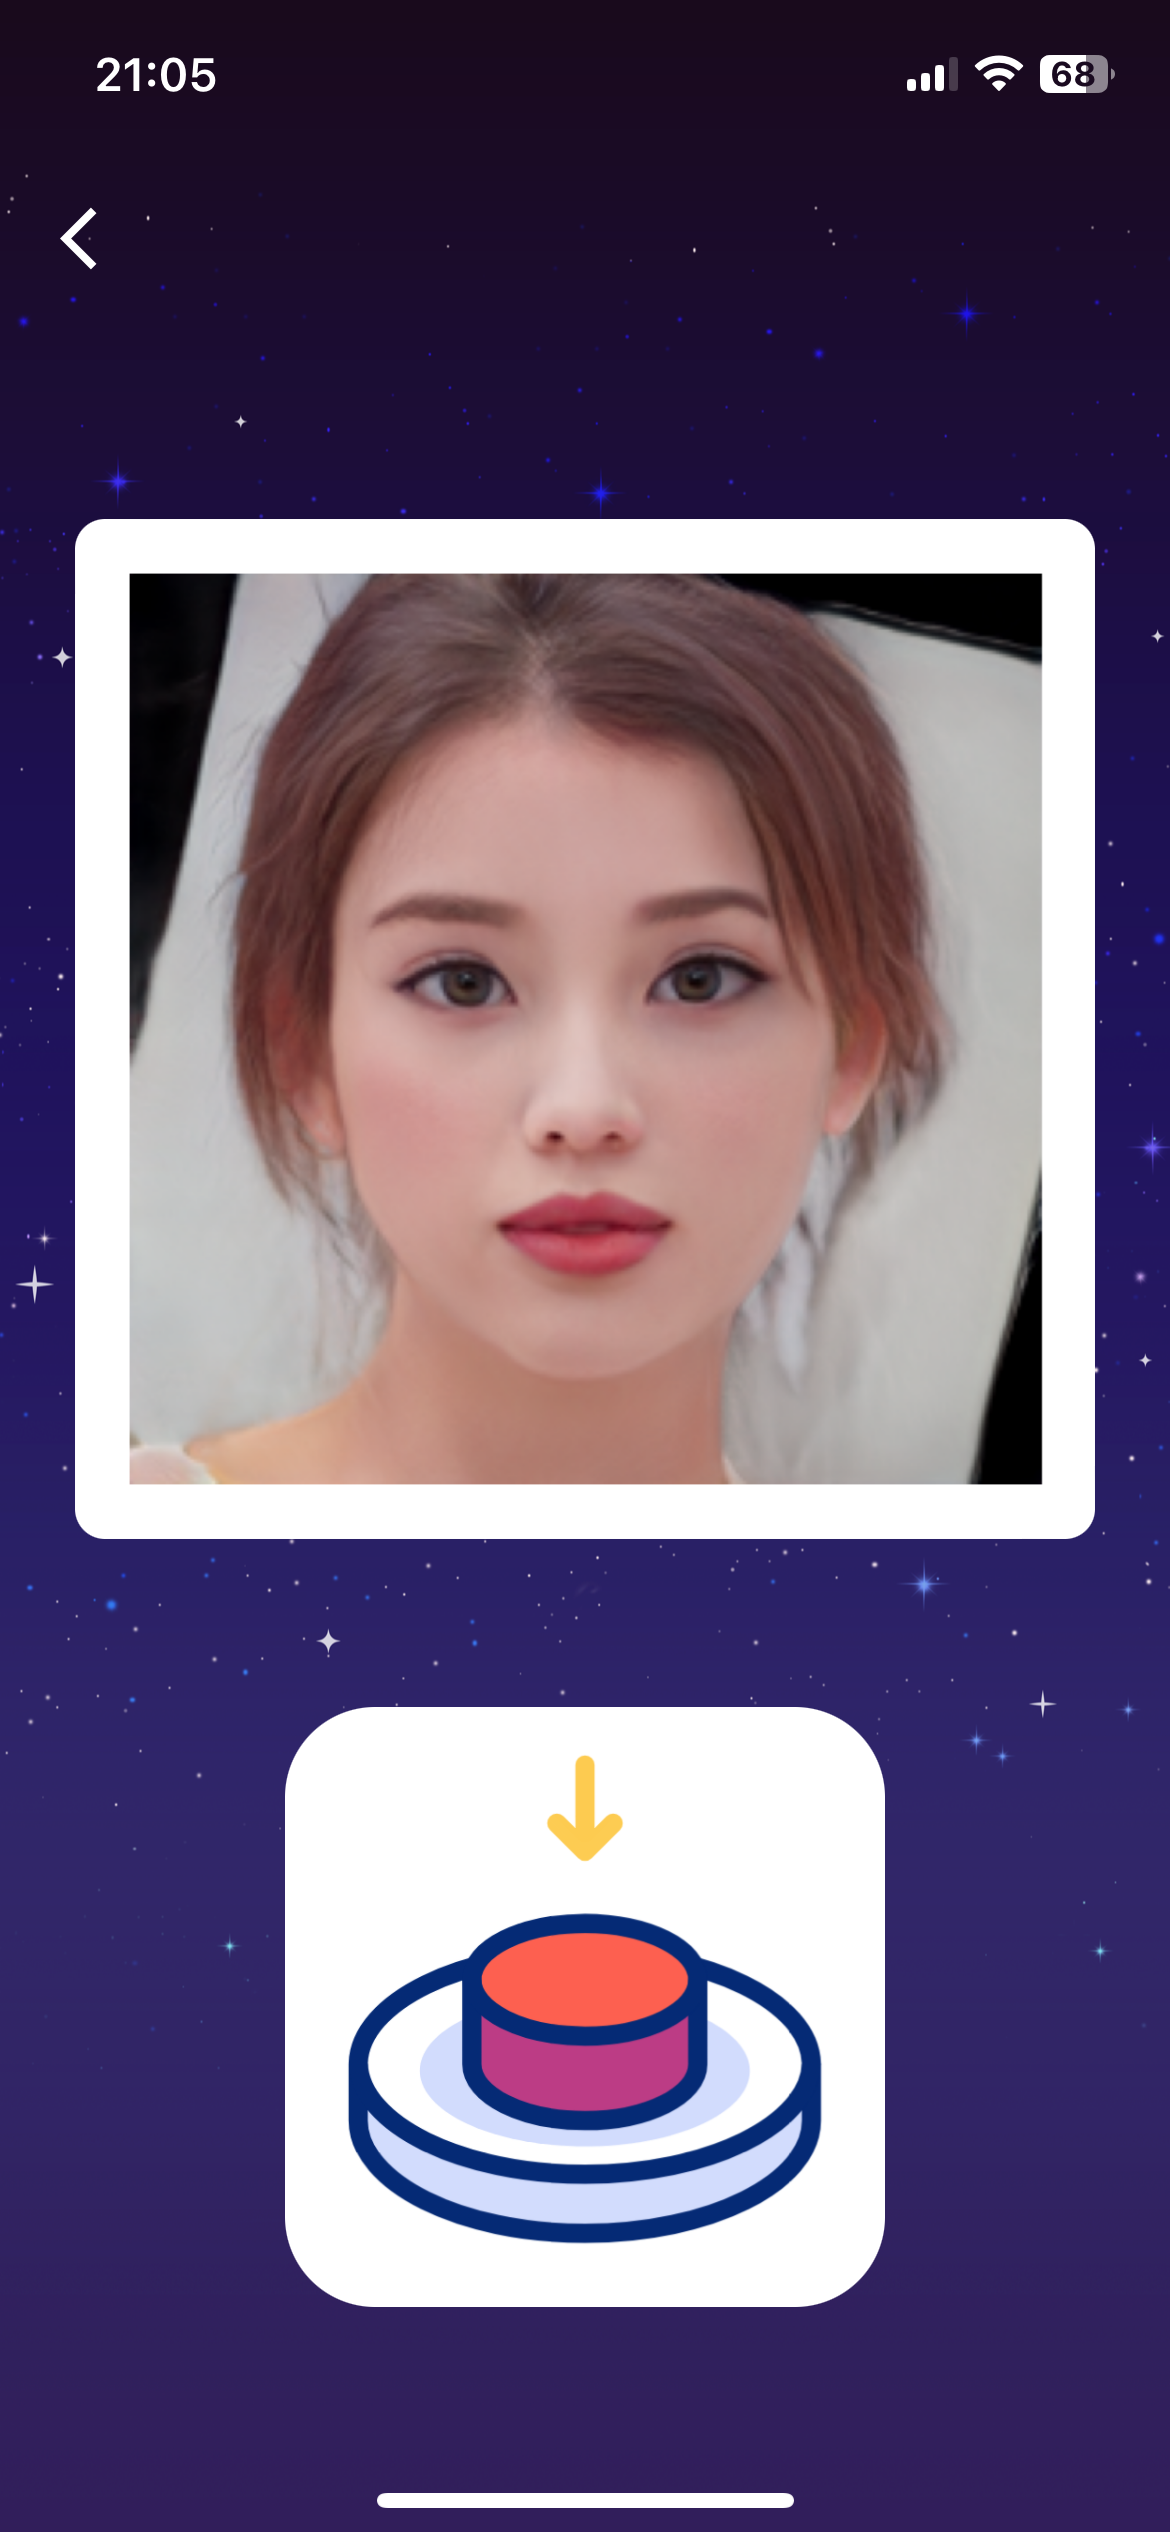
\includegraphics[width=3cm]{Images/screen/game/disney/DISNEY2_PLAYER.PNG}}
            \caption{AI Guessing Game}
            \label{fig}
        \end{figure}
        When the operator of the app runs the toonify AI code, the original and result photo files are stored in the problem and answer folders of AWS S3 cloud storage with ascending numerical filenames. When a user requests the AI guessing game in the app, the backend randomly selects a number, generates URLs for the number.png files in the problem and answer folders, and sends them in JSON format.\\
        When the game host presses the game start button, the first toonified image photo received in JSON format appears simultaneously on the screens of both the game host and the player. In order of arrival, players guess the answer, and when the game host presses the 'Check Answer' button, the correct answer text (character name) appears, and the Toonified image transforms into the original image. When the game host presses the 'Next Question' button, the next toonified image appears, and the game continues in the same manner.\\
        The AI model for the AI guessing game utilizes the StyleGAN2 model to toonify the given photo input. Initially, when a photo is received, the crop code processes it to ensure facial features are appropriately positioned in the photo. The cropped photo is then used to train a model that generates human facial images similar to the input photo using the pre-trained StyleGAN2 generation model. The newly generated model is combined with another pre-trained model, the toonify face model, to create a toonified image. The toonify image can be adjusted by modifying the alpha value to control the degree of toonification. The generated image is finally stored in AWS S3 in the form of a photo.

    \subsection{Geography Guessing Game}
        \begin{figure}[htbp]
            \centerline{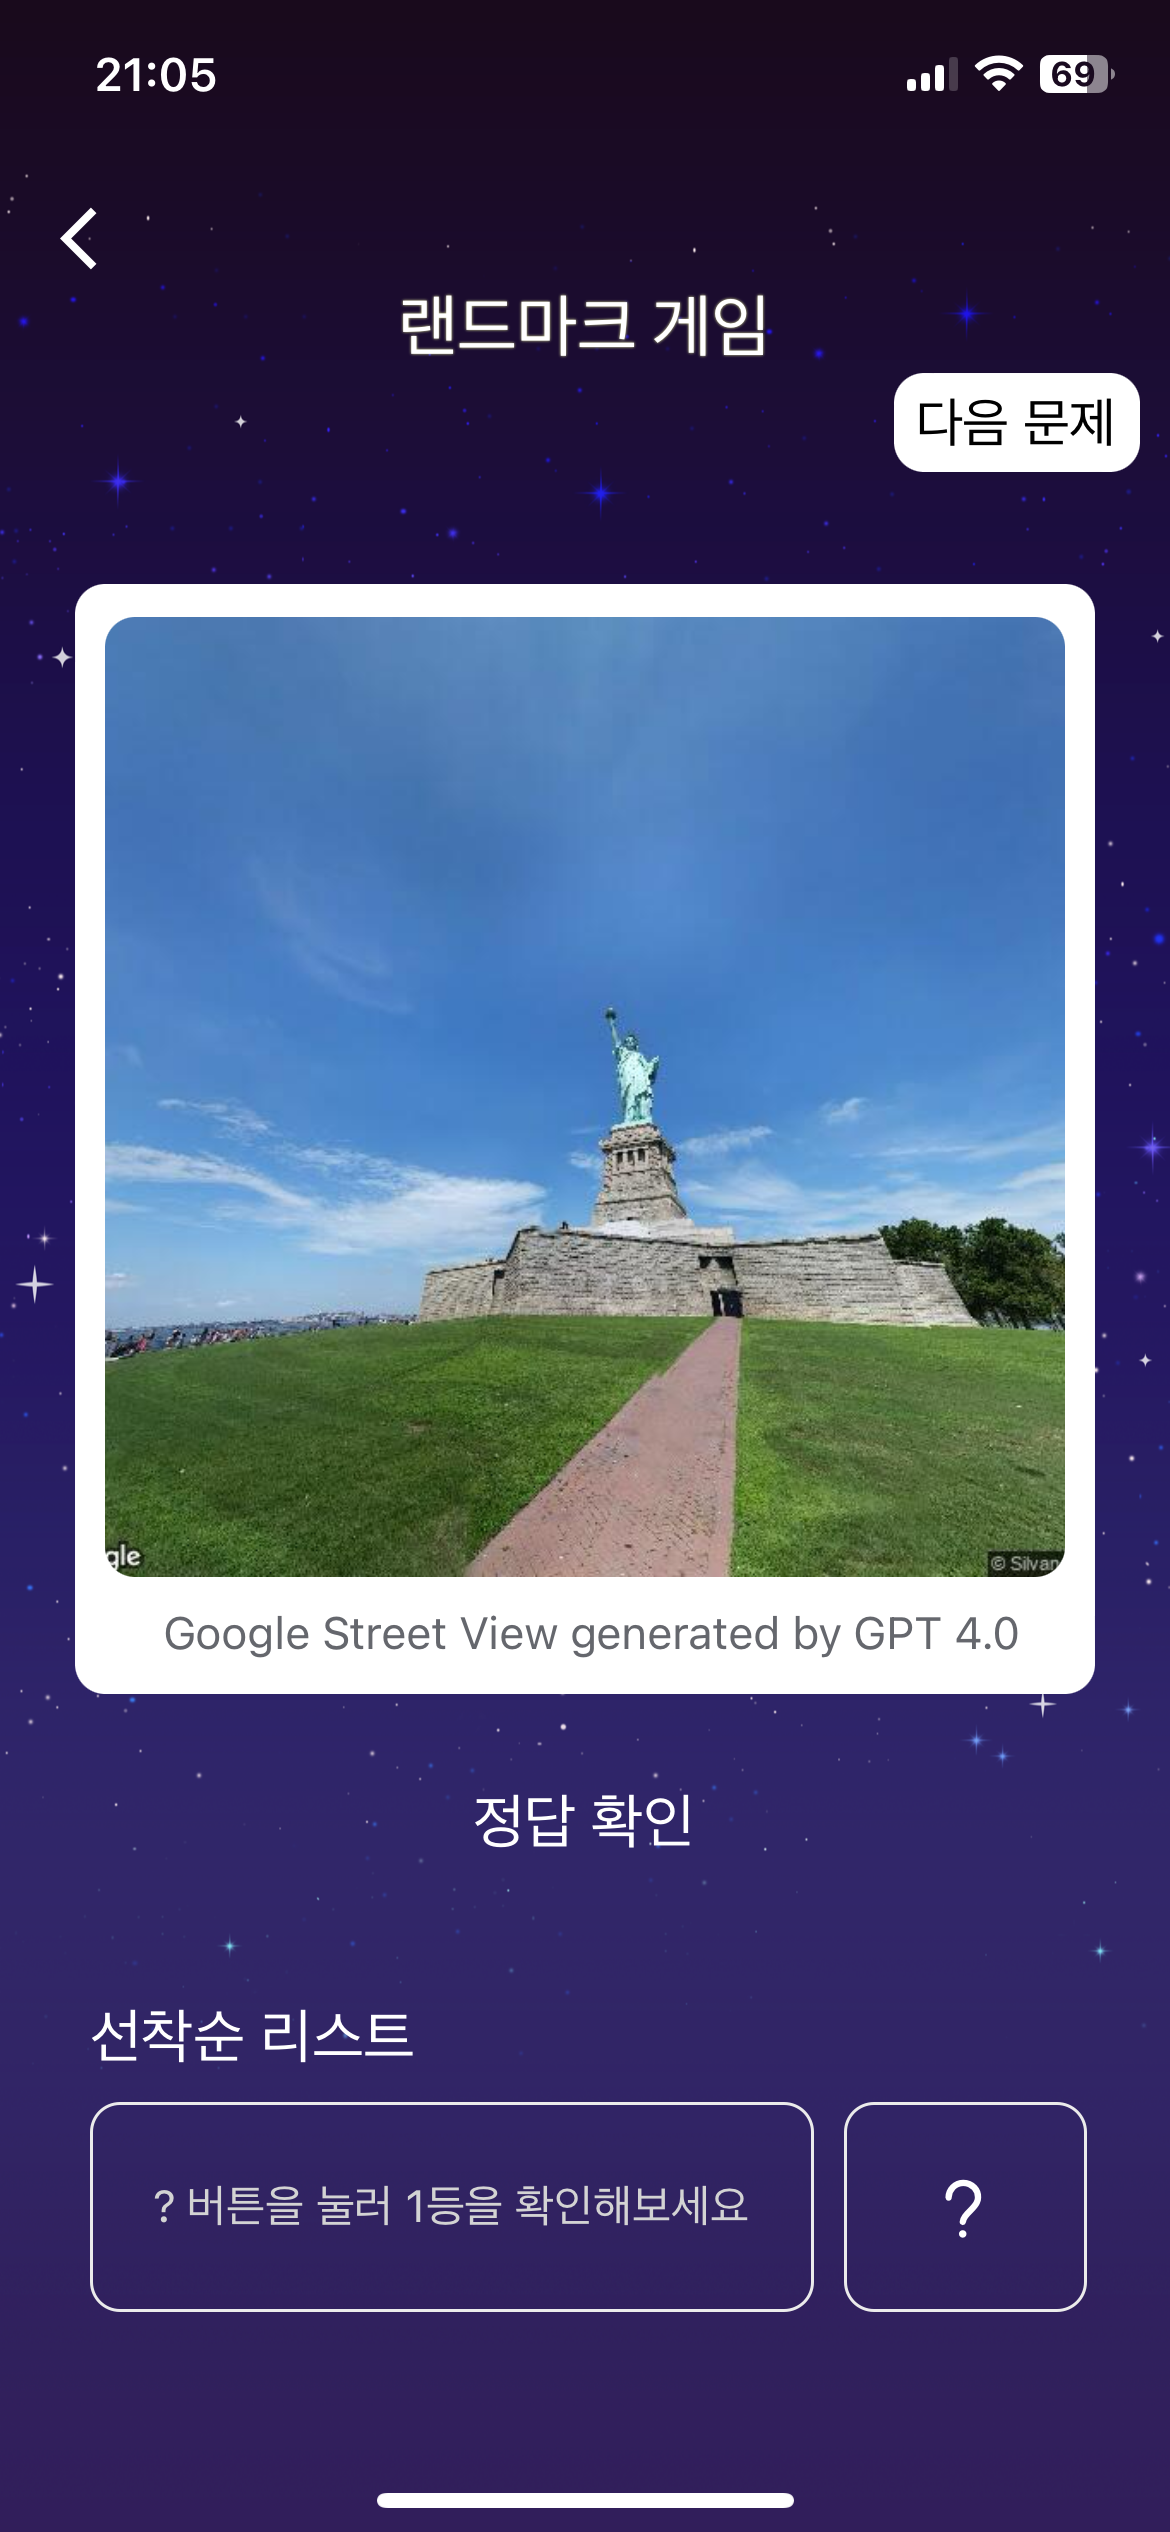
\includegraphics[width=3cm]{Images/screen/game/geo/GEO2_HOST.PNG}
            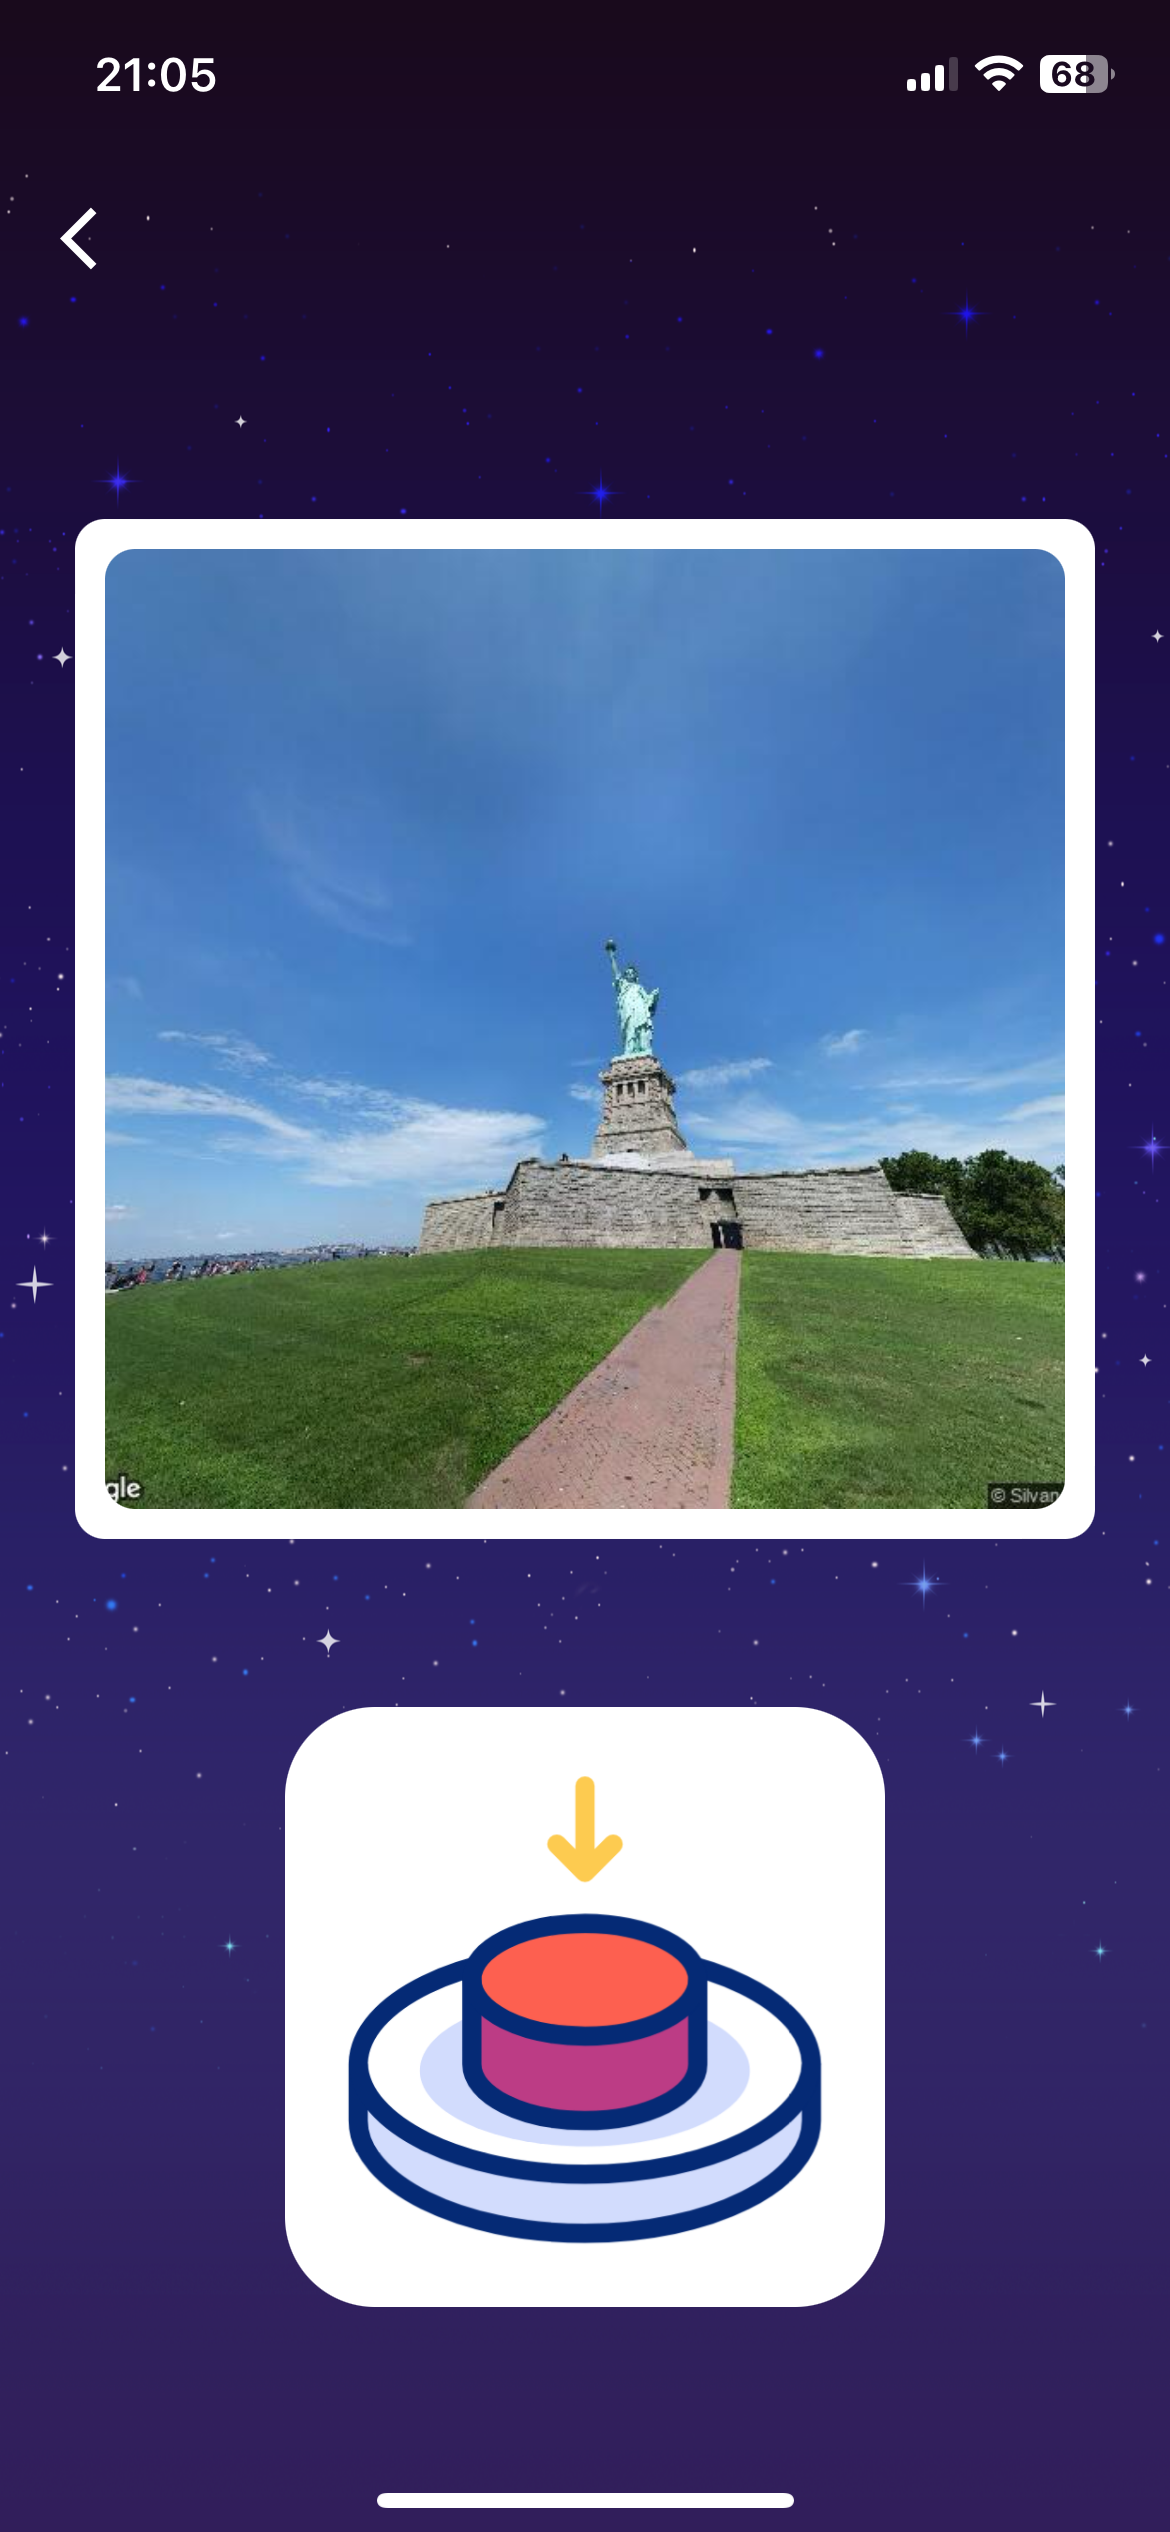
\includegraphics[width=3cm]{Images/screen/game/geo/GEO2_PLAYER.PNG}}
            \caption{Geography Guessing Game}
            \label{fig}
        \end{figure}
        In the app, when a user requests a game, it retrieves values such as latitude and longitude of world-famous landmarks from the OpenAI API. Using the obtained values and the Google Street View API, it sends the URL of the Street View image of the famous landmark in JSON format.\\
        When the game host presses the game start button, the images of the famous landmarks received in JSON format simultaneously appear on the screens of both the game host and the player. By the order of pressing the answer button,, players guess the answer, and when the game host presses the 'Check Answer' button, the name of the landmark appears on the screen. When the game host presses the 'Next Question' button, the next landmark image appears, and the game continues in the same manner.

    \subsection{'Gather Up' Game}
        \begin{figure}[htbp]
            \centerline{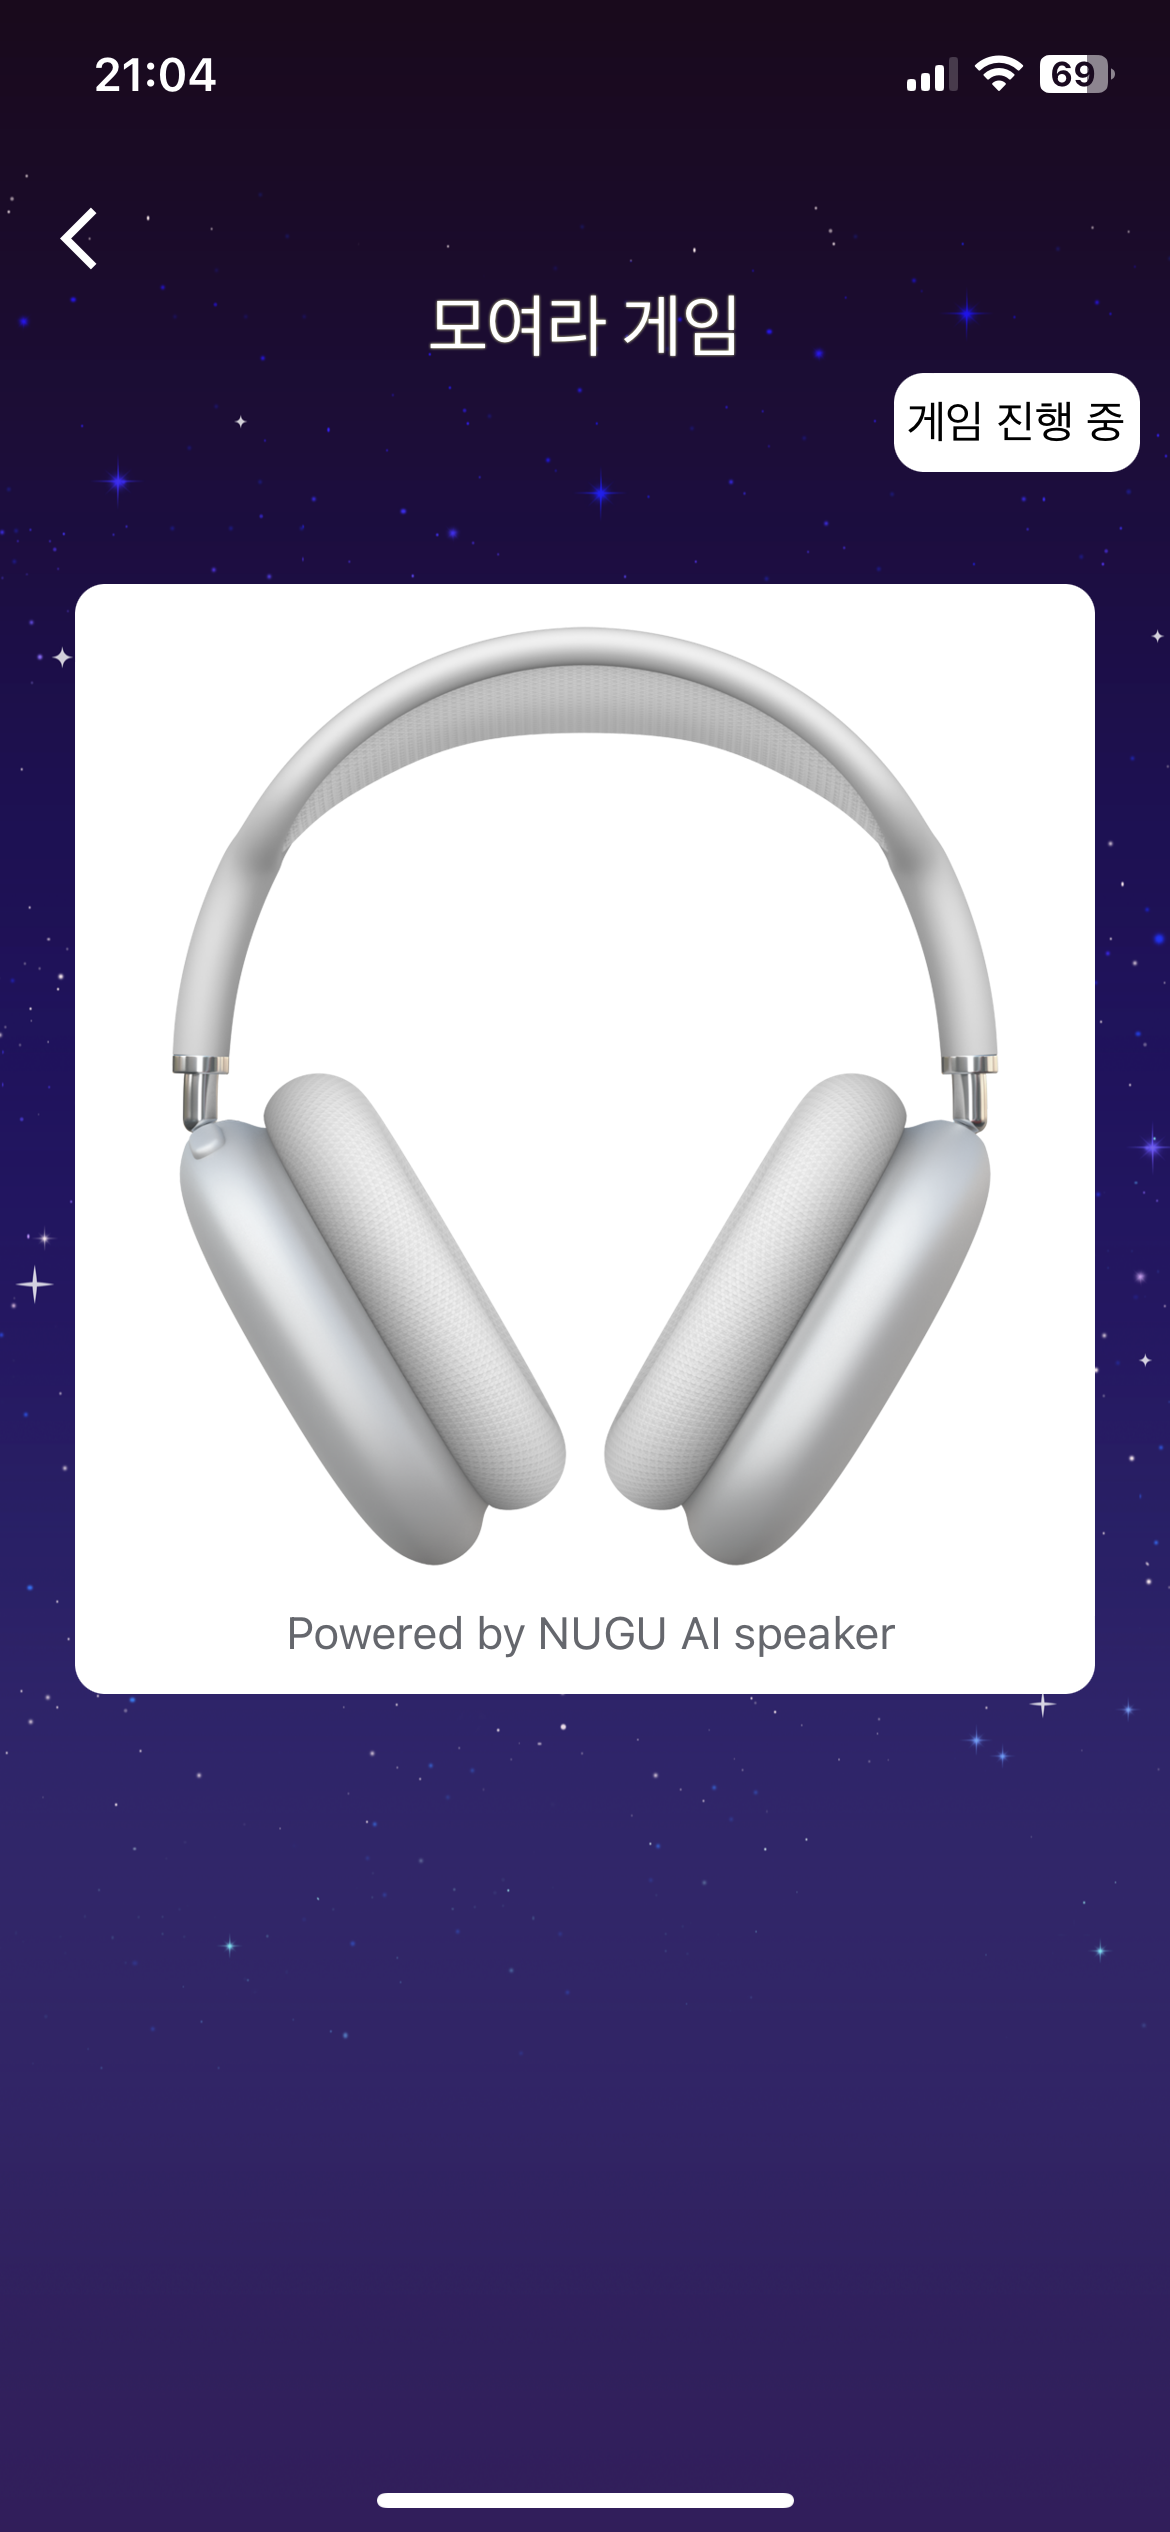
\includegraphics[width=3cm]{Images/screen/game/gather/GATHERUP.PNG}
            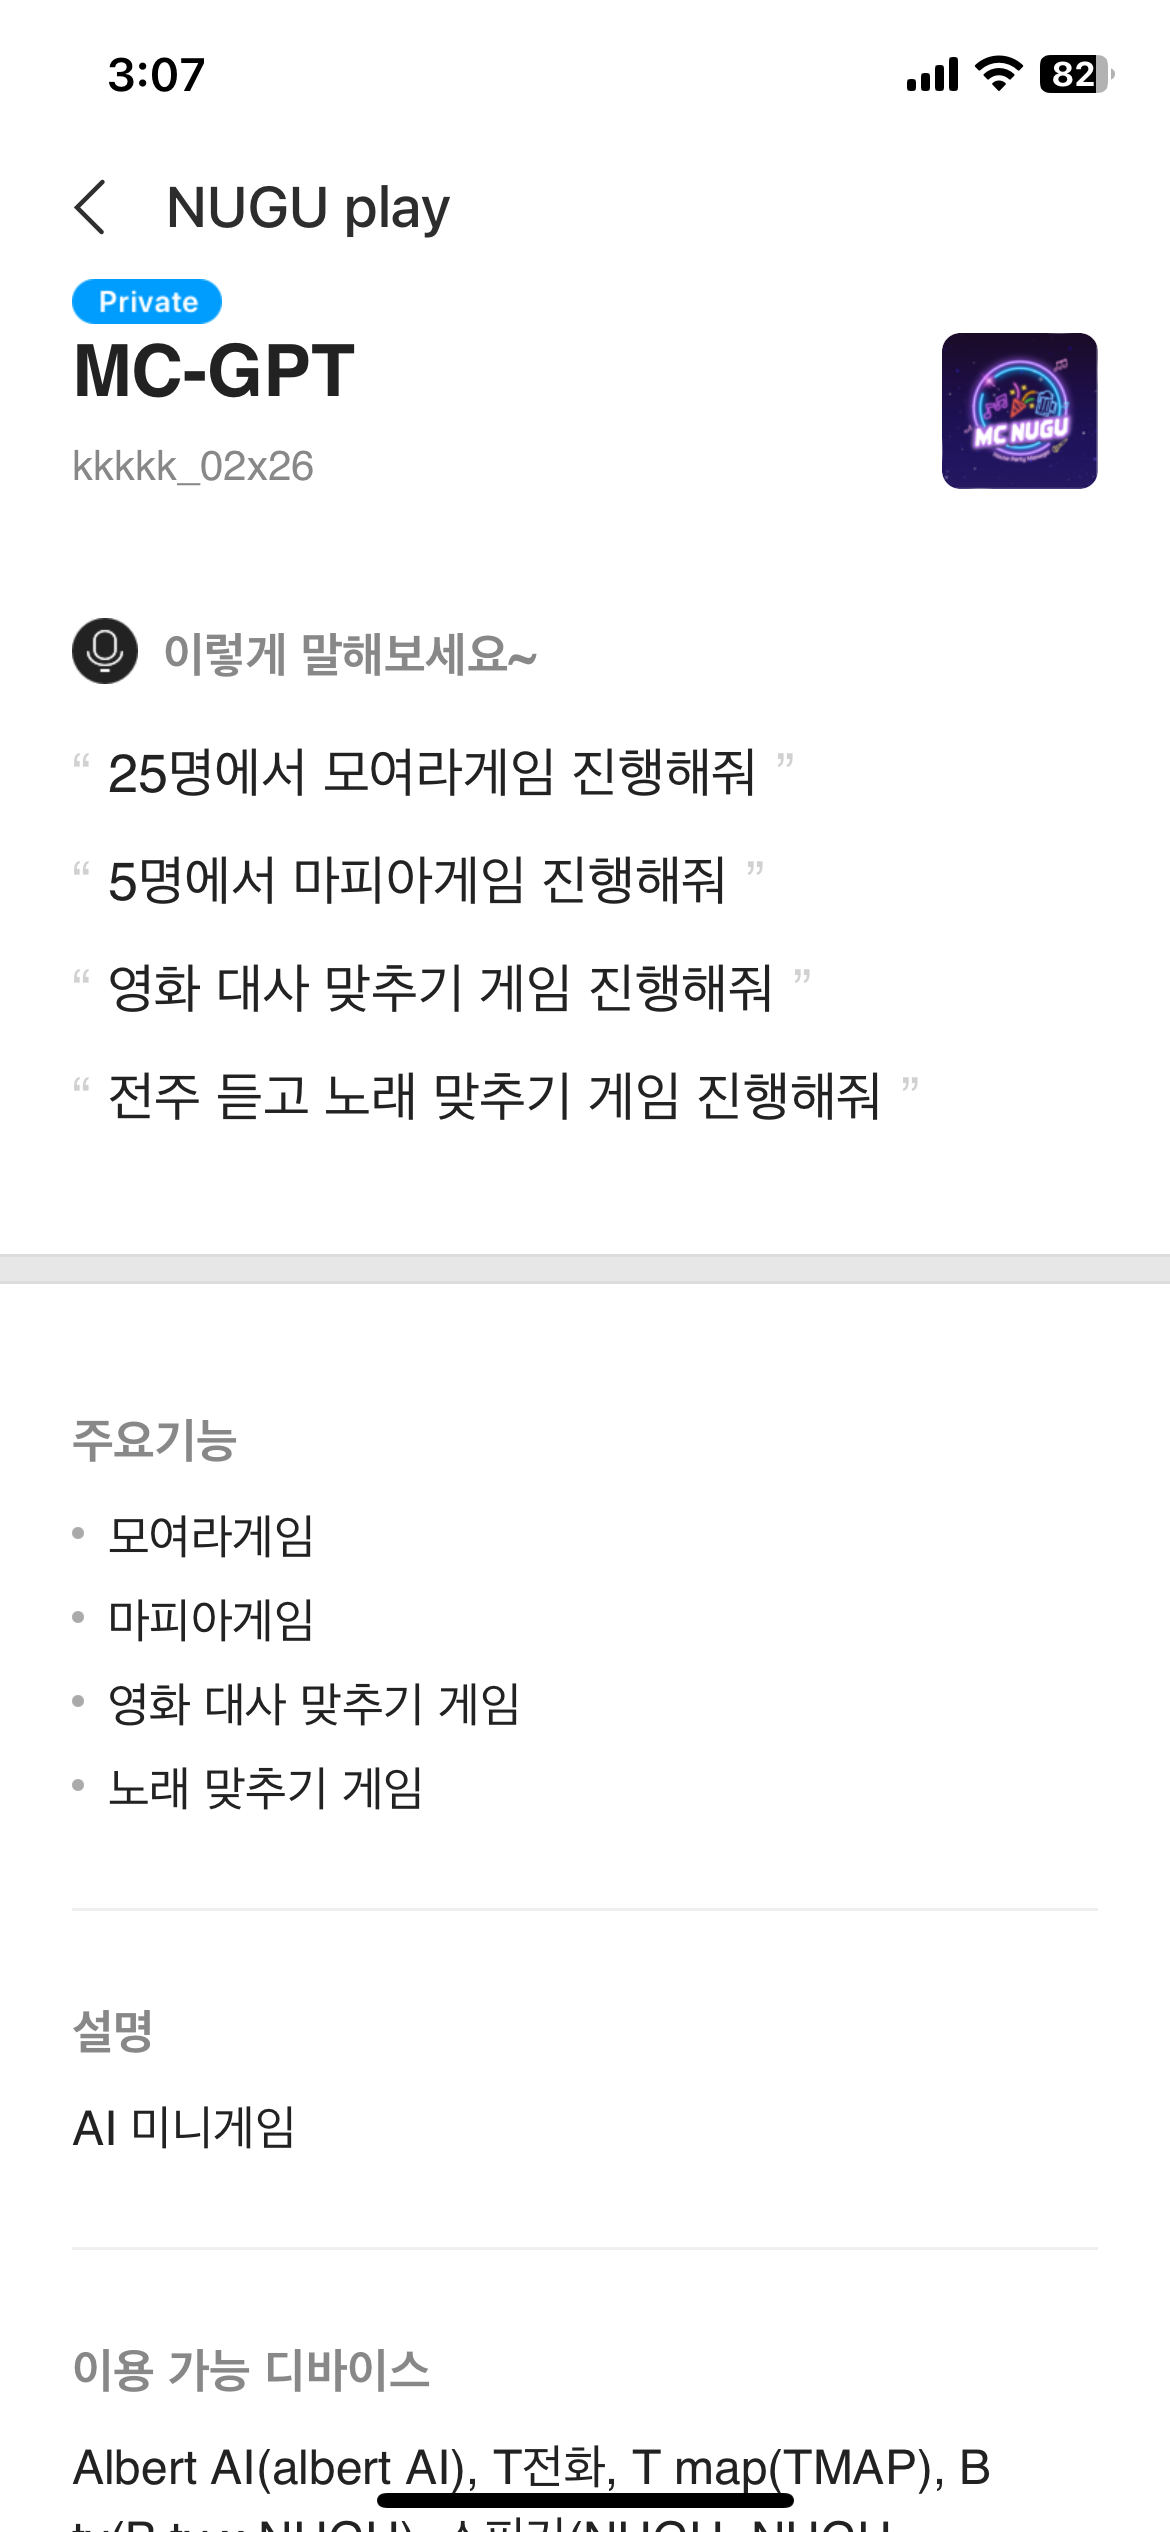
\includegraphics[width=3cm]{Images/screen/game/gather/NUGU_Playbuilder.png}}
            \caption{Gather Up}
            \label{fig}
        \end{figure}
        Using the NUGU AI Speaker, commands such as 'Start a game with 25 people.' can be given. The speaker sends the number '25' to the connected backend. The backend, using its own algorithm, returns a suitable number for the gathering game. The speaker then responds with something like '6 people gather up!' based on the algorithm's output.
        
    \subsection{App Setting Page}
        \begin{figure}[htbp]
            \centerline{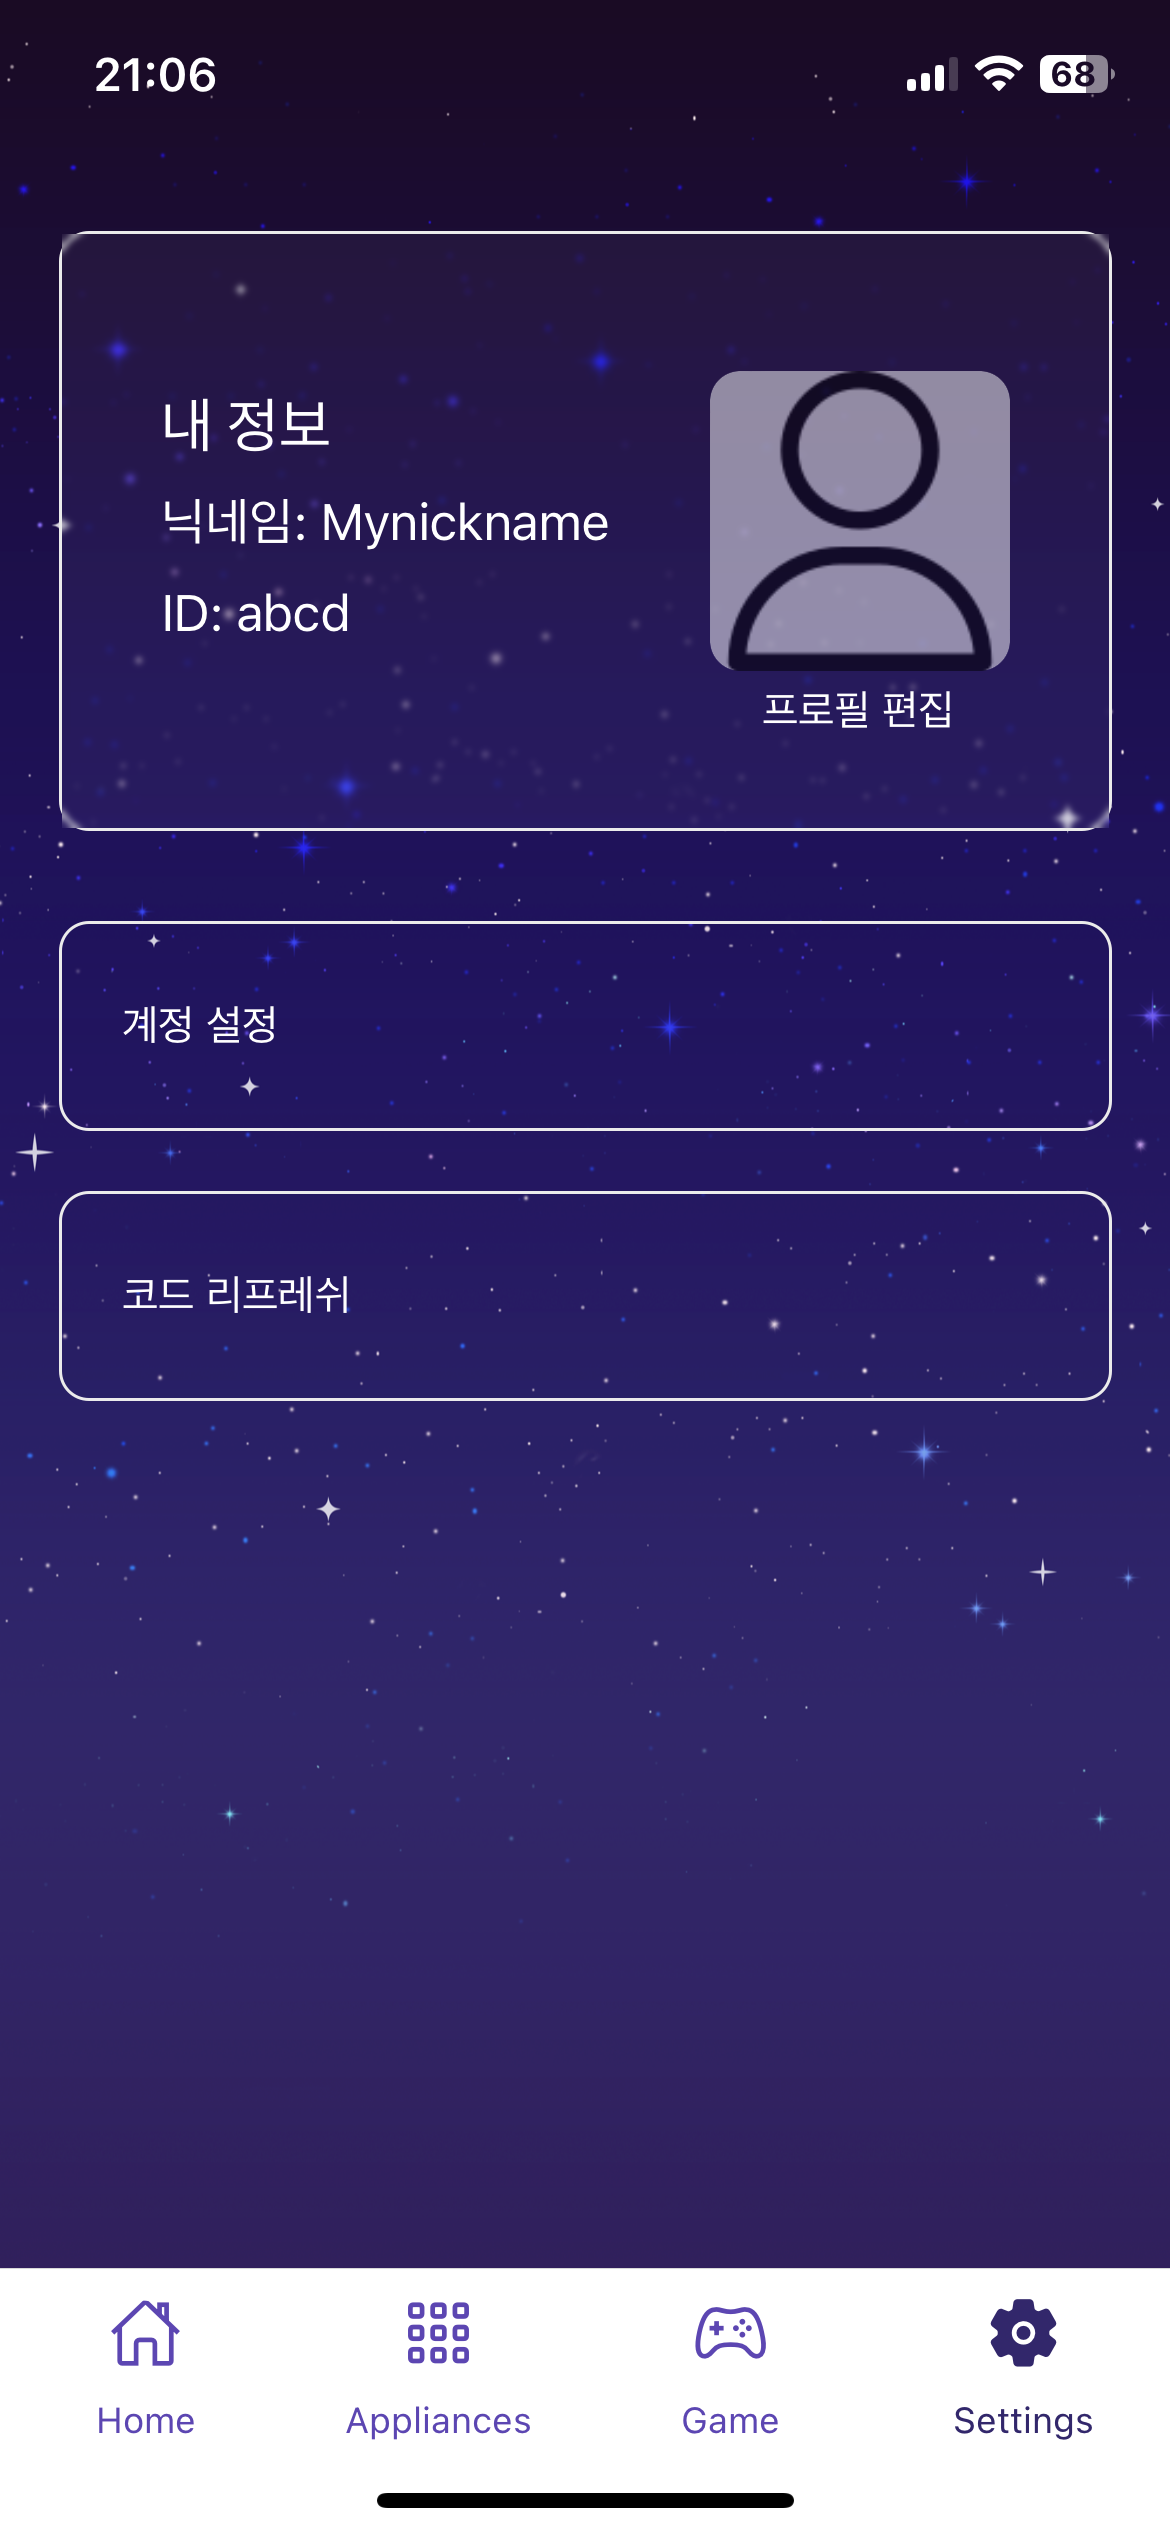
\includegraphics[width=3cm]{Images/screen/settings/SETTING_HOST.PNG}
            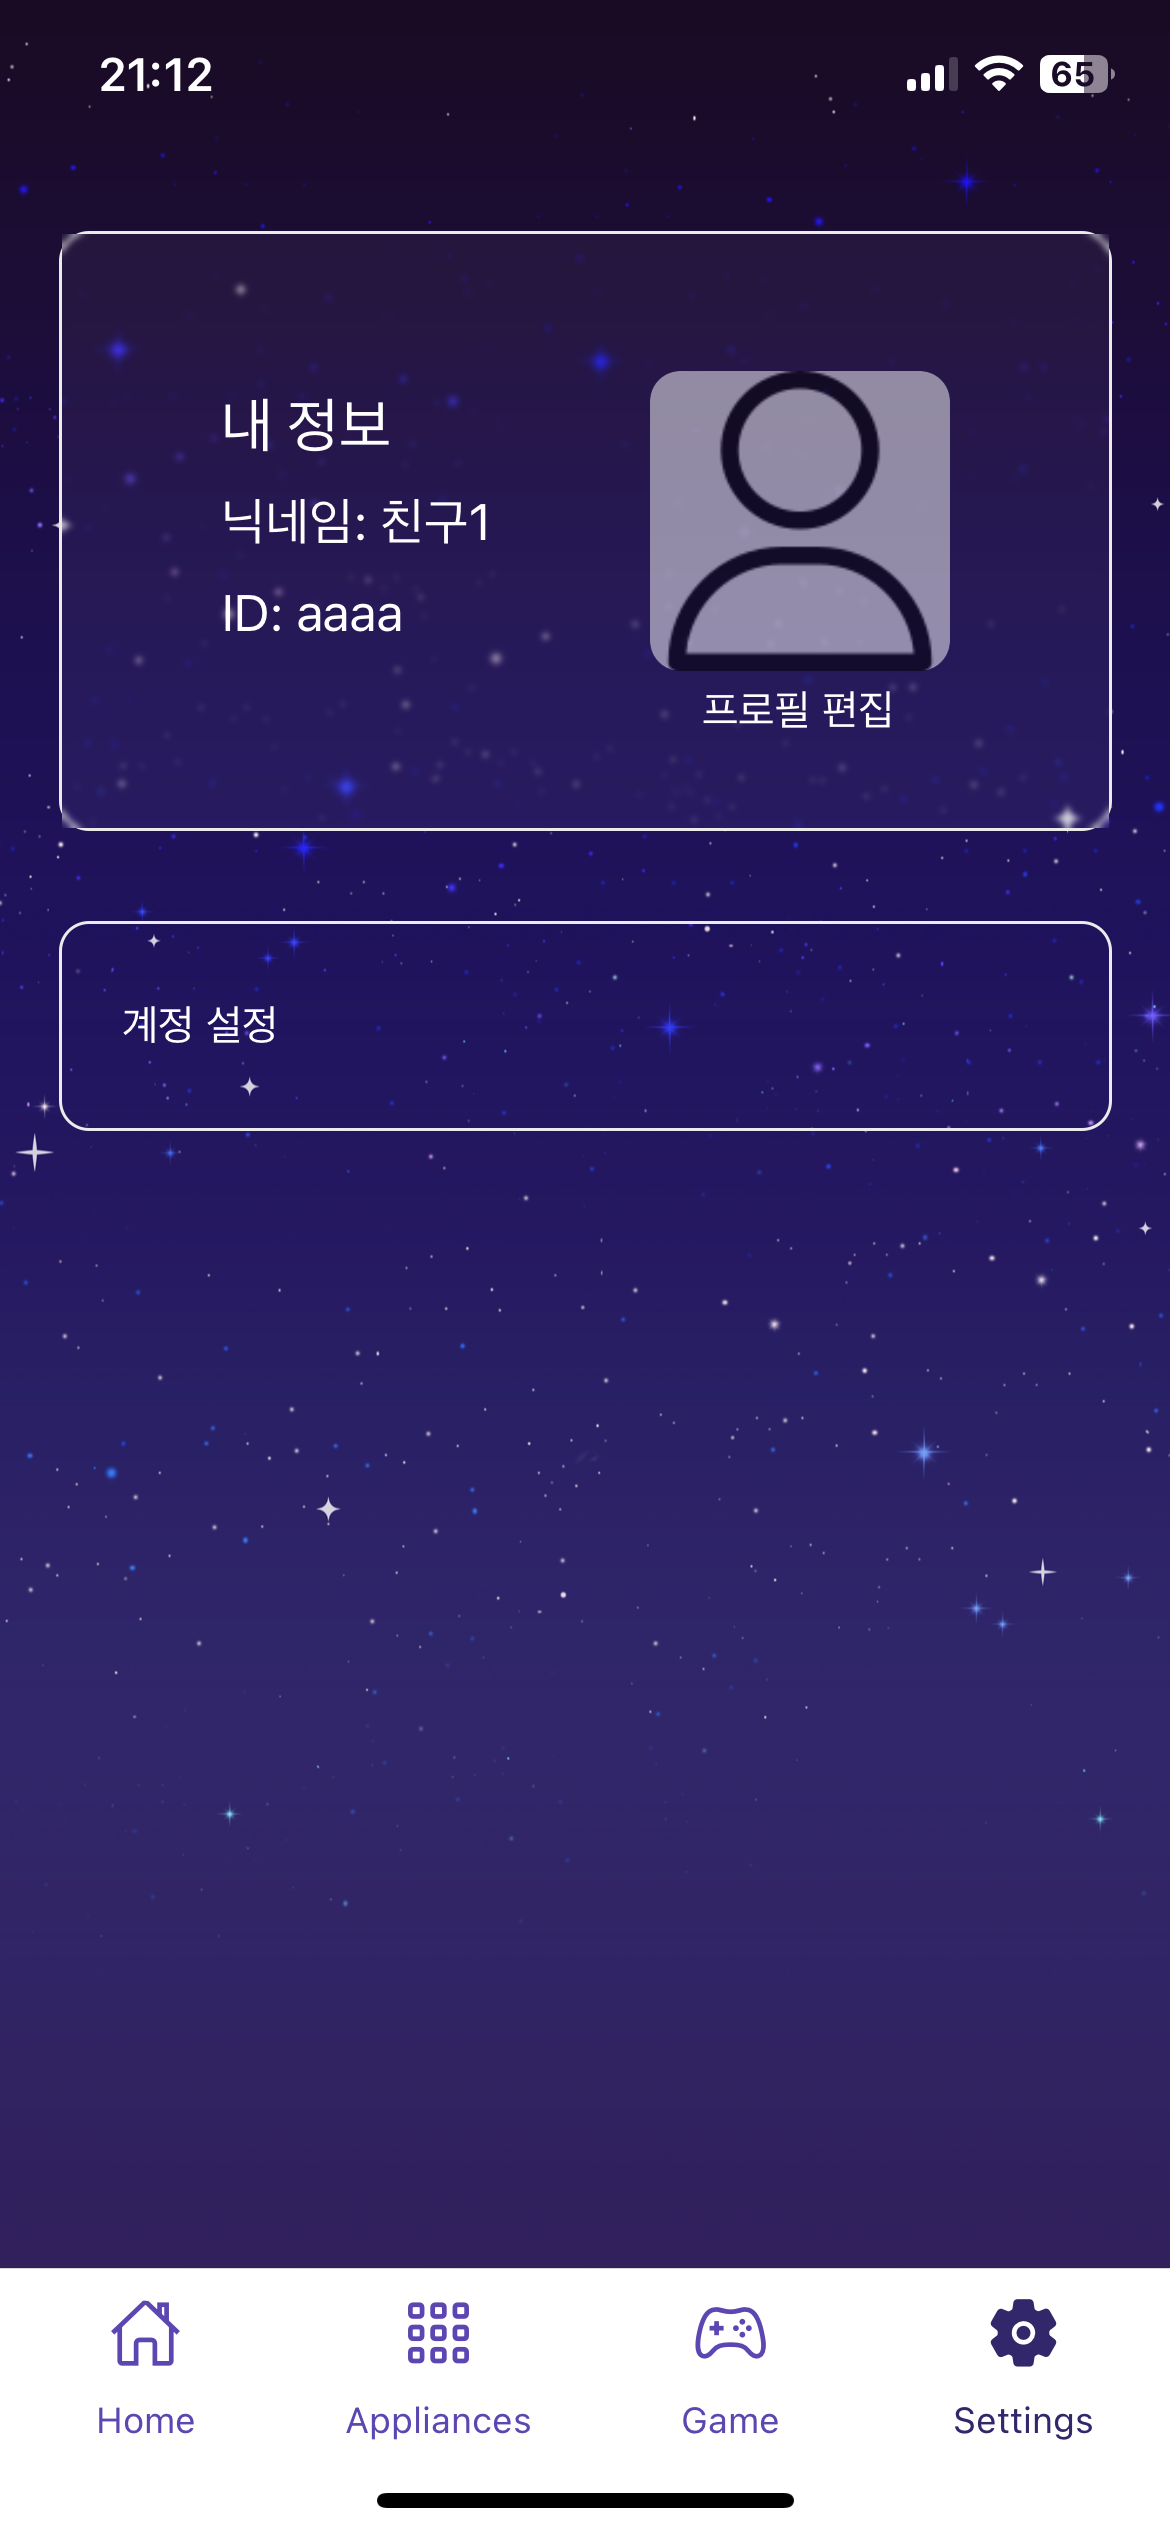
\includegraphics[width=3cm]{Images/screen/settings/SETTING_GUEST.PNG}}
            \caption{App Setting Page}
            \label{fig}
        \end{figure}
        App setting page is a page where any kind of settings regarding the app can be modified, such as logging out. The main difference and function of the application’s setting is that it has buttons regarding the refreshing of the space code.\\
        When you press the "Code Refresh" button, the room's access code is randomly changed, and at the same time, all guests who were invited to the room are removed.\\
        Pressing the "Code Refresh" button causes all user's room access permissions to expire, and they are redirected to the room selection screen.

\section{Architecture Design}
    \subsection{Overall Architecture}
        Our service consists of four modules: front-end, back-end, database and AI
            \begin{figure}[htbp]
                \centerline{\includegraphics[width = 8cm]{Images/archi/overall.png}}
                \label{fig}
                \caption{Overall Architecture}
            \end{figure}
            The first module is the frontend that directly interacts with the user. The frontend of MC GPT is designed and developed using the React Native framework and Expo CLI. Users can access servers, databases, and artificial intelligence speakers through the app. The MC GPT app represents login, registration, room information, lighting and appliance information, game information, and account information through communication with the backend server via HTTP.\\
            In the lighting control feature, it is connected to ChatGPT to receive party lighting color information and implement the recommendation of party lighting colors for users. The game feature is implemented by connecting to the server using WebSocket, allowing multiple people to enjoy party games such as Disney games, geography games, and gather games in real-time. Among these, the gather game is connected to the artificial intelligence speaker when entering the game.\\
            React Hooks were utilized to manage local state and handle events. The Context API was used to access globally used states and values, allowing access from multiple screens. Through this, the app achieves consistent state management and data sharing, providing users with a more cohesive experience.\\
            \begin{figure}[htbp]
                \centerline{\includegraphics[width = 9cm]{Images/archi/erd.png}}
                \label{fig}
                \caption{Database Diagram}
            \end{figure}
            The second module is the backend that interacts with the database. The backend of MC GPT consists of a main server implemented in Spring, a second server implemented in Flask, a database implemented in PostgreSQL, and AWS S3 cloud storage. The main server has functionalities such as login and registration, creation, retrieval, modification, and deletion of spaces and appliances, and real-time game progress. Various data generated through user interaction in the application is stored in the database through the main server. Among various games, the game utilizing the NUGU speaker goes through the algorithm of the main server, and the response is delivered to the speaker.\\
            The second server handles game and AI-related functions. For Disney games, the images generated by AI are uploaded to AWS S3. The server extracts 10 random links to these images from the storage and sends them to the frontend in link format. For geography games, the server receives latitude, longitude, and other values of famous tourist spots from the OpenAI API, uses them with the Google Street View API, and sends 10 links at a time to the frontend. The main server utilizes real-time communication features to progress the game using the links returned by the second server.\\
            All these backend components are built on the Amazon Web Services (AWS) cloud computing platform. The main server and the second server are implemented on separate AWS Compute Cloud (Elastic EC2) instances, and the database is included in the EC2 instance of the main server.\\
            \vspace{3mm}
            
            The third module is the machine learning module for the AI image game. The primary functionality of the AI code is to process and manipulate photos for games on the game tab, creating generative image files and changing original photos to resemble Disney characters. Anything related to photos is processed using the StyleGAN2 model. To utilize the StyleGAN2 model, AI frameworks such as PyTorch and Tensorflow are employed.\\
            The main script is the core component, establishing a connection to an AWS S3 bucket and performing tasks such as cropping, image inversion, and applying a toonify effect. It attempts to upload the resulting toonified image to the "MC-GPT" S3 bucket.\\
            The projector defines an image inversion process using a pre-trained StyleGAN2-based generator. It iteratively adjusts a latent code to generate an image close to a given input face image. The result is saved to an output path, utilizing the LPIPS library for perceptual loss calculation.\\
            The toonify file defines an image toonification process using two pre-trained StyleGAN2-based generators. It blends intermediate outputs of corresponding layers in the generators to create a toonified image.\\
            The model defines a PyTorch implementation of a StyleGAN2-based generator (Generator class) and discriminator (Discriminator class) for image generation tasks. It includes functionalities for image blending, patch swapping, and merging, enhancing the generator's versatility.\\

            
    \subsection{Directory Organization}
    \subsection{Module 1: Front-End}
        \subsubsection{Purpose}
            We wanted to make the house party more colorful through the Generative AI. AI speaker and application are the ways in which the user reaches the Generative AI. Frontend's application was developed based on the React Native. React Native enables cross-platform development and offers plenty of libraries and functionalities, simplifying the development process. Using Expo, developers can check the actual execution screen while creating the app. This application facilitates user-server connections to store user-entered values in the backend and retrieve data from backend-provided databases for user viewing.\\
            \vspace{3mm}
        \subsubsection{Functionality}
            Separating the space between a party host and a party guest, Displaying party-related appliances states on frontend screens, Control the lighting to match the lighting theme generated by the Generative AI, Managing the party mini games generated by Generative AI, and basic functions to support users such as signup, login authentication, account settings connected with backend servers.\\
            \vspace{3mm}
        \subsubsection{Location of source code}
            \begin{itemize}
                \item  github.com/MC-GPT/Frontend
            \end{itemize}
            
            \begin{table}[]
                \centering
                \caption{Frontend Directory}
                \begin{tabular}{p{2cm}|p{2.6cm}|p{3.2cm}}
                    \hline
                    \textit{\textbf{Directory}} & \textit{\textbf{File Name}} & \textit{\textbf{Modules Used}}\\ 
                    \hline 

                    \begin{tabular}[t]{@{}l@{}}
                    MC-GPT/\end{tabular} & 
                    \begin{tabular}[c]{@{}l@{}}             assets\\src\\.eslintrc.json\\.prettierrc\\App.js\\app.json\\babel.config.js\\package-lock.json\\package.json \end{tabular} \\
                    \hline

                    \begin{tabular}[c]{@{}l@{}}
                    MC-GPT/assets/\end{tabular} & 
                    \begin{tabular}[c]{@{}l@{}}                    background.png\\brightness.png\\Button\_off.png\\Button\_on.png\\color.png\\Disney.png\\Gatherup.png\\Geo.png\\icon.png\\mcnugulogo.png\\NewJeans.png\\nugu\_neon.gif\\nugu\_neon.png\\onoff.png\\play.png\\profile.png\\vote.gif\\\end{tabular} \\
                    \hline

                    \begin{tabular}[c]{@{}l@{}}
                    MC-GPT/assets/\\app/\\\end{tabular} & 
                    \begin{tabular}[c]{@{}l@{}}                    AirConditioner.png\\AirPurifier.png\\Beer.png\\disco-ball.png\\GameConsole.png\\GameJoystick.png\\Hanger.png\\HomeTheater.png\\KitchenLight.png\\Lamp.png\\LightBulb.png\\MoodupFridge.png\\Shower.png\\Speaker.png\\Standbyme.png\\WashingMachine.png\\\end{tabular} \\
                    \hline

                    \begin{tabular}[c]{@{}l@{}}
                    MC-GPT/src/\end{tabular} & 
                    \begin{tabular}[c]{@{}l@{}}                    
                    App.js\\color.js\end{tabular} \\
                    \hline

                    \begin{tabular}[c]{@{}l@{}}
                    MC-GPT/src/\\components/\end{tabular} & 
                    \begin{tabular}[c]{@{}l@{}}                    Button.js\\Input.js\\Popup.js\\PopupB.js\\SafeInputView.js\\TextAnimation.js\\TextButton.js\\\end{tabular} &
                    \begin{tabular}[c]{@{}l@{}}                    
                    react\\react-native\\prop-types\\expo/vector-icons \end{tabular} \\
                    \hline

                    \begin{tabular}[c]{@{}l@{}}
                    MC-GPT/src/\\contexts/\end{tabular} & 
                    \begin{tabular}[c]{@{}l@{}}                    GameContexts.js\\MainContext.js\\UserContext.js\\\end{tabular} &
                    \begin{tabular}[c]{@{}l@{}}                    
                    react\\prop-types\\ \end{tabular} \\
                    \hline

                    \begin{tabular}[c]{@{}l@{}}
                    MC-GPT/src/\\screens\\\end{tabular} & 
                    \begin{tabular}[c]{@{}l@{}}                    ElectroInfoScreen.js\\ElectronicScreen.js\\GameListScreen.js\\GameManageScreen.js\\GamePlayScreen.js\\HomeScreen.js\\LightningScreen.js\\LoadingScreen.js\\MoodLightScreen.js\\RoomScreen.js\\SettingsScreen.js\\SignInScreen.js\\SignUpScreen.js\\\end{tabular} &
                    \begin{tabular}[c]{@{}l@{}}                    
                    react\\react-native\\prop-types\\expo/vector-icons\\react-navigation/native\\react-native-safe-area-\\context\\expo-blur\\axios\\ \end{tabular} \\
                    \hline                    
        
                \end{tabular}
            \end{table}
            \begin{table}[]
                \centering
                \begin{tabular}{p{2cm}|p{2.6cm}|p{3.2cm}}
                \hline
                    \begin{tabular}[c]{@{}l@{}}
                    MC-GPT/src/\\navigations\\\end{tabular} & 
                    \begin{tabular}[c]{@{}l@{}}                    Appliances.js\\AuthStack.js\\ContentTab.js\\index.js\\MainStack.js\\\end{tabular} &
                    \begin{tabular}[c]{@{}l@{}}                    
                    react-native\\expo/vector-icons\\react-navigation/material-\\top-tabs\\react-native-safe-area-context\\react-navigation/native\\react-navigation/native-stack\\react-navigation/bottom-tabs \end{tabular} \\
                \hline
                \end{tabular}
            \end{table}
        \subsubsection{Component}
            \begin{itemize}
                \item MC-GPT/ : This folder contains frontend source code of MC-GPT service.
                    \item[-] .prettierrc : prettier is a code formatting tool that developers can use to automatically format their code using preset guidelines. 
                    \item[-] .eslintrc.json : ESlint is a tool for identifying and reporting on patterns found in ECMAScript/JavaScript code, with the goal of making code more consistent and avoiding bugs.
                \vspace{3mm}
                
                \item MC-GPT/assets : This folder contains images and font files used within the app.
                \vspace{3mm}
                
                \item MC-GPT/src : This folder is the main folder containing components, contexts, navigation, and screens.
                    \item[-] App.js : This file is a root component that is wrapped in the providers of context API for global state management.
                    \item[-] colors.js : This file contains information about colors used throughout the app. This exported file is used to manage the colors that are mainly used at once. 
                \vspace{3mm}
                
                \item MC-GPT/src/components : This folder contains custom components created using basic components. By utilizing custom components, development can be facilitated by combining frequently used components for app development.
                    \item[-] Button.js : This Button component is a custom component for frequently used primary buttons. It receives props such as title, onPress, onLongPress, disabled, isLoading, styles, and buttonType to define custom buttons that vary depending on the purpose of use.
                    \item[-] Input.js : This Input component is a custom component created by adding an icon, keyboard type, etc. to the text input component provided by React Native. It also added a function that emphasizes the boundaries of the window that the user is entering and a function that operates the keyboard.
                    \item[-] Popup.js : This Pop-up component is a custom component created by adding an input window and text based on the modal window provided by React Native.
                    \item[-] SafeInputView.js : This SafeInputView component is a custom component that adds the ability to make the keyboard disappear based on KeyboardAvoidingView provided by React Native.
                    \item[-] TextAnimation.js : This TextAnimation component is a custom component for moving text effects. This component was used to show notice in Homescreen. This text animation moves in a minute from the left end to the right end of the screen.
                    \item[-] TextButton.js : This TextButton component is a custom component created by adding style based on the Pressable component provided by React Native. It can be used throughout the app, so it is designed to apply the style at once.
                \vspace{3mm}
                
                \item MC-GPT/src/contexts : The context api is configured to manage the state which is used in the app service globally.
                    \item[-] GameContext.js : Game context is a component that defines game-related state variables and functions used globally.
                    \item[-] MainContext.js : Main context defines the global state variables used across the app.
                    \item[-] UserContext.js : User context is a global status management code that manages information related to a user and tokens used for backend communication.
                \vspace{3mm}
                
                \item MC-GPT/src/navigations
                    \item[-] Appliances.js : Appliances is a navigation that goes beyond the light list screen and the non-light list screen of home appliances.
                    \item[-] AuthStack.js : Authstack is a navigation that contains not-logged-in screens. It consists of LoginScreen and SignupScreen.
                    \item[-] ContentTab.js : Content tab is a navigation used for bottom tab navigation. It consists of Home, Appliance, Game, and Settings screens
                    \item[-] index.js : index is a navigation that separates and moves MainStack screens that are logged in and AuthStack screens that are not logged in.
                    \item[-] MainStack.js : MainStack is a navigation for moving between screens using stack navigator. It includes RoomScreen, HomeScreen, ContentTab, MoodLightScreen, ElectroInfoScreen, SettingsScreen, GamePlayScreen, GameManageScreen.
                \vspace{3mm}
                
                \item MC-GPT/src/screens
                    \item[-] ElectroInfoScreen.js : The ElectroInfoScreen is a screen that controls the detailed operation of the non-light home appliances.
                    \item[-] ElectronicScreen.js : The ElectronicScreen is a screen that displays, adds, and deletes a list of non-light home appliances. 
                    \item[-] GameListScreen.js : The GameListScreen is a screen that displays a list of party games on the screen through game information received from the server.
                    \item[-] GameManageScreen.js : The GameMangeScreen is a screen that appears after a game host creates a game room. It consists of a web socket code for playing the game in real time and a code for managing the game play.
                    \item[-] GamePlayScreen.js : The GamePlayScreen is a screen that appears after a player who participates in a game enters the game room. It consists of a web socket code to play the game in real time and a code that appears in the game play.
                    \item[-] HomeScreen.js : The HomeScreen is a screen that appears when a user enters a room for the first time. Information about the room, such as the name of the room and the invitation code, and the home appliance dashboard appear. The part that controls music played on artificial intelligence speakers is also composed of codes.
                    \item[-] LightningScreen.js : The LightningScreen allows lighting lists to appear and create and delete lighting. Simple on-off and locking features are also designed.
                    \item[-] LoadingScreen.js : The Loading Screen represents a loading image to be displayed on the screen while receiving information from the server.
                    \item[-] MoodLightScreen.js : The MoodLightScreen is a screen that controls the detailed operation of the lightning appliances.
                    \item[-] RoomScreen.js : The RoomScreen is a screen that displays room lists received from the server divided into MyHome and Guest. The user can create a room in the MyHome part and add a guest room through the invitation code in the Guest part.
                    \item[-] SettingsScreen.js : The SettingsScreen is a screen showing a user's profile and account information. The owner of the room can update the invitation code and initialize the guest through the Code Refresh function.
                    \item[-] SignInScreen.js : SignInScreen is a screen that displays the input window and buttons required for a user to log in and implements a login function.
                    \item[-] SignUpScreen.js : SignUpScreen is a screen that displays the input window and buttons required for a user to sign up and implements a signup function.
            \end{itemize}    
        
    \subsection{Module 2: Back-End}
        \subsubsection{Purpose} 
            The backend server generates a response by interacting with the database when a request is made from the frontend. When data entered in the frontend is sent to the backend in JSON format, the backend processes the data by performing create, read, update, and delete operations on the database, and then generates a response in JSON format. The generated response is then delivered to the MC-GPT app.\\
            \vspace{3mm}
        \subsubsection{Functionality}
            The backend server performs computations, communicates with NUGU, provides real-time gaming functionality, and interacts with the database. Additionally, it retrieves and returns appropriate responses to frontend requests by interacting with the database.\\
            \vspace{3mm}
        \subsubsection{Location of source code}
            \begin{itemize}
                \item Main Server : github.com/MC-GPT/Backend
                \item Second Server : github.com/MC-GPT/Backend-for-AI
            \end{itemize}

            \begin{table}[]
                \centering
                \caption{Backend Directory}
                \begin{tabular}{p{2.4cm}|p{2.8cm}|p{2.7cm}}
                    \hline
                    \textit{\textbf{Directory}} & \textit{\textbf{File Name}} & \textit{\textbf{Modules Used}}\\ 
                    \hline 

                    \begin{tabular}[c]{@{}l@{}}
                    MC-GPT/\end{tabular} & 
                    \begin{tabular}[c]{@{}l@{}}
                    src/main\\build.gradle\end{tabular} \\
                    \hline

                    \begin{tabular}[c]{@{}l@{}}
                    MC-GPT/src/main/\end{tabular} & 
                    \begin{tabular}[c]{@{}l@{}}
                    java/com.aise.mcnugu\\resources\end{tabular} \\
                    \hline

                    \begin{tabular}[c]{@{}l@{}}
                    MC-GPT/src/main/\\resources/\\\end{tabular} & 
                    \begin{tabular}[c]{@{}l@{}}
                    application.properties\end{tabular} \\
                    \hline

                    \begin{tabular}[c]{@{}l@{}}
                    MC-GPT/src/main/\\java/com.aise.com/\\\end{tabular} & 
                    \begin{tabular}[c]{@{}l@{}}                    config\\controller\\domain\\dto\\repository\\service\\websocket\\McNuguApplication.java \end{tabular} &
                    \begin{tabular}[c]{@{}l@{}}
                    SpringBootAppli-\\cation\end{tabular} \\
                    \hline

                    \begin{tabular}[c]{@{}l@{}}
                    MC-GPT/src/main/\\java/com.aise.mcnugu/\\config/\\\end{tabular} & 
                    \begin{tabular}[c]{@{}l@{}}                    jwt\\SecurityConfig.java\\WebSocketConfig.java\end{tabular} &
                    \begin{tabular}[c]{@{}l@{}}                    Configuration\\EnableWebSecurity\\EnableWebSocket\\RequiredArgsConstructor\\Bean \end{tabular} \\
                    \hline

                    \begin{tabular}[c]{@{}l@{}}
                    MC-GPT/src/main/\\java/com.aise.mcnugu/\\config/jwt/\\\end{tabular} & 
                    \begin{tabular}[c]{@{}l@{}}                    TokenInfo.java\\JwtTokenProvider.java\\JwtAuthentication-\\Filter.java\\CustomUserDetails-\\Service.java\\\end{tabular} &
                    \begin{tabular}[c]{@{}l@{}}                    Builder\\Data\\AllArgsConstructor\\Component\\RequiredArgsConstructor\\Service\\Slf4j \end{tabular} \\
                    \hline

                    \begin{tabular}[c]{@{}l@{}}
                    MC-GPT/src/main/\\java/com.aise.mcnugu/\\config/controller/\\\end{tabular} & 
                    \begin{tabular}[c]{@{}l@{}}                    MemberContoller.java\\HomeController.java\\ApplianceController.java\\GuestController.java\\NuguController.java\end{tabular} &
                    \begin{tabular}[c]{@{}l@{}}                    RestController\\RequiredArgsConstructor\\Slf4j \end{tabular} \\
                    \hline

                    \begin{tabular}[c]{@{}l@{}}
                    MC-GPT/src/main/\\java/com.aise.mcnugu/\\config/domain/\\\end{tabular} & 
                    \begin{tabular}[c]{@{}l@{}} Member.java\\Authority.java\\Home.java\\Appliance.java\\Guest.java\\Game.java\\Home\_Game.java\\\end{tabular} &
                    \begin{tabular}[c]{@{}l@{}}                    Entity\\Getter\\Setter\\AllArgsConstructor\\NoArgsConstructor\\Builder\\ \end{tabular} \\
                    \hline

                    \begin{tabular}[c]{@{}l@{}}
                    MC-GPT/src/main/\\java/com.aise.mcnugu/\\config/dto/\\\end{tabular} & 
                    \begin{tabular}[c]{@{}l@{}}                         nugu\\SignupRequest.java\\LoginRequest.java\\CreateHomeRequest.java\\MainResponse.java\\CreateAppRequest.java\\GameRoomRequest.java\end{tabular} &
                    \begin{tabular}[c]{@{}l@{}}                    
                    Getter\\Builder \end{tabular} \\
                    \hline

                    \begin{tabular}[c]{@{}l@{}}
                    MC-GPT/src/main/\\java/com.aise.mcnugu/\\config/dto/nugu/\\\end{tabular} & 
                    \begin{tabular}[c]{@{}l@{}}                    NuguActionDto.java\\NuguGatherUpDto.java\\NuguReturnDto.java\end{tabular} &
                    \begin{tabular}[c]{@{}l@{}}
                    Getter\\Setter\\NoArgsConstructor \end{tabular} \\
                    \hline

                    \begin{tabular}[t]{@{}l@{}} 
                    MC-GPT/src/main/\\java/com.aise.mcnugu/\\config/repository/\\\end{tabular} & 
                    \begin{tabular}[c]{@{}l@{}}                    MemberRepository.java\\HomeRepository.java\\ApplianceRepository.java\\GuestRepository.java\\GameRepository.java\\Home\_Game-\\Repository.java\end{tabular} &
                    \begin{tabular}[c]{@{}l@{}}                    JPARepository \end{tabular} \\
                    \hline

                    \begin{tabular}[c]{@{}l@{}}
                    MC-GPT/src/main/\\java/com.aise.mcnugu/\\config/service/\\\end{tabular} & 
                    \begin{tabular}[c]{@{}l@{}}                    MemberService.java\\HomeService.java\\ApplianceService.java\\GuestService.java\end{tabular} &
                    \begin{tabular}[c]{@{}l@{}}                    
                    Service\\RequiredArgsConstructor\\Transactional\\Slf4j \end{tabular} \\
                    \hline

                    \begin{tabular}[c]{@{}l@{}}
                    MC-GPT/src/main/\\java/com.aise.mcnugu/\\config/websocket/\\\end{tabular} & 
                    \begin{tabular}[c]{@{}l@{}}                    GameRoom.java\\Message.java\\GameRoomService.java\\GameRoomController.java\\WebSocketHandler.java\end{tabular} &
                    \begin{tabular}[c]{@{}l@{}}                            Getter\\Setter\\Component\\Service\\RestController\\RequiredArgsConstructor\\Slf4j\\ \end{tabular} \\
                    \hline

                \end{tabular}
            \end{table}
                        
        \subsubsection{Component}
            \begin{itemize}
                \item Main Server (MC-GPT/Backend)
                    \item[-]build.gradle : This file is a build configuration for the project. It contains a set of plugins and dependencies essential for the proper execution of the Spring Boot application.
                \vspace{3mm}
                
                \item src/resources/application.properties : This file manages settings used in Spring projects. It includes configurations such as database connection details, server port, and other application-specific properties.
                \vspace{3mm}
                
                \item src/main/java/com.aise.mcnugu/config : This package contain additional configuration files for the Spring application. It includes general application configuration, beans, and other settings.
                    \item[-] SecurityConfig.java : A configuration file for Spring Security, specifying security-related settings for the application.
                    \item[-] WebSocketSecurity.java : WebSocket-specific security configuration.
                \vspace{3mm}
                
                \item src/main/java/com.aise.mcnugu/config/jwt : This package contain files regarding jwt which used for authentication.
                    \item[-] TokenInfo.java : A class that holds information about authentication tokens.
                    \item[-] JwtTokenProvider.java : A class responsible for handling JWT authentication.
                    \item[-] JwtAuthenticationFilter.java : A filter to process JWT authentication.
                    \item[-] CustomUserDetailsService.java : A custom implementation of Spring Security’s UserDetailsService interface.
                \vspace{3mm}
                
                \item src/main/java/com.aise.mcnugu/config/controller/ : This is a package that contains files that process user requests and then hand over model objects to the specified view.
                    \item[-] MemberContoller.java : An API controller handling API requests related to managing users.
                    \item[-] HomeController.java : An API controller managing API requests related to spaces.
                    \item[-] ApplianceController.java : An API controller dealing with API requests related to managing LG and other appliances.
                    \item[-] GuestController.java : An API controller managing API requests related to creating relationships between users and spaces.
                    \item[-] NuguController.java : An API controller handling API requests related to the NUGU AI Speaker.
                \vspace{3mm}
                
                \item src/main/java/com.aise.mcnugu/config/domain/ : This is a package folder that contains all the entity files.
                    \item[-] Member.java : An entity class representing users.
                    \item[-] Authority.java : An entity class representing user authority.
                    \item[-] Home.java : An entity class representing spaces.
                    \item[-] Appliance.java : An entity class representing LG and other appliances.
                    \item[-] Guest.java : An entity class representing relationship between user and space.
                    \item[-] Game.java : An entity class representing mini-game.
                    \item[-] Home\_Game.java : An entity class representing relationship between spaces and mini-game.
                \vspace{3mm}
                
                \item src/main/java/com.aise.mcnugu/config/dto/ : This is a package that contains the Data Transfer Object files.
                    \item[-] SignupRequest.java : This is a class of json mapped to object from frontend to create member.
                    \item[-] LoginRequest.java : This is a class of json mapped to object from frontend to logging in.
                    \item[-] CreateHomeRequest.java : This is a class of json mapped to object form frontend to create home.
                    \item[-] MainResponse.java : This is a class that contains the values to be returned when entering space.
                    \item[-] CreateAppRequest.java : This is a class of json mapped to object from frontend to create appliance.
                    \item[-] GameRoomRequest.java : This is a class of json mapped to object from frontend to create game room.
                    \item[-] NuguGatherUpDto.java : This is a dto to calculate GatherUp game algoritm.
                    \item[-] NuguReturnDto.java : This is a dto to be returned to NUGU. It contains the version of backend proxy server, resultCode, and output.
                \vspace{3mm}

                \item src/main/java/com.aise.mcnugu/config/repository/ : This is a package that contains files that use JPA to access database.
                    \item[-] MemberRepository.java : This is a file accessing database by JPA to ‘member’ table.
                    \item[-] HomeRepository.java : This is a file accessing database by JPA to ‘home’ table.
                    \item[-] ApplianceRepository.java : This is a file accessing database by JPA to ‘appliance’ table.
                    \item[-] GuestRepository.java : This is a file accessing database by JPA to ‘guest’ table.
                    \item[-] GameRepository.java : This is a file accessing database by JPA to ‘game’ table.
                    \item[-] Home\_GameRepository.java This is a file accessing database by JPA to ‘home\_game’ table.
                \vspace{3mm}

                \item src/main/java/com.aise.mcnugu/config/service/ : This is a package that contains business logic files.
                    \item[-] MemberService.java : A file containing business logic related to users.
                    \item[-] HomeService.java : A file containing business logic related to spaces.
                    \item[-] ApplianceService.java : A file containing business logic related to LG and other appliances.
                    \item[-] GuestService.java : A file containing business logic related to creating guests for spaces.
                \vspace{3mm}

                \item  src/main/java/com.aise.mcnugu/config/websocket/ : This is a package that contains related to real-time service using websocket.
                    \item[-] GameRoom.java : An entity class representing GameRoom.
                    \item[-] Message.java : An entity class representing Message.
                    \item[-] GameRoomService.java : A file containing business logic related to game room.
                    \item[-] GameRoomController.java : An API controller managing API requests related to game room.
                    \item[-] WebSocketHandler.java : This is a file that handle websocket events, such as user connections, disconnections, and facilitating real-time communication.
                \vspace{3mm}

                \item Second Server (MC-GPT/Backend-for-AI/)
                    \item[-] app.py : This file define the routes, endpoints and behavior for the second API server.
                    \item[-] gpt.py : This file contains code related to OpenAI API, indicating functionality for natural language processing or text generation.
                    \item[-] streetview.py : This file handle functionality related to street view, interacting with Google Street View API.

                
            \end{itemize}
        
    \subsection{Module 3: Database}
        \subsubsection{Purpose}
            MC-GPT utilizes a significant amount of data, including user, space, home appliance, and game data. To ensure the operation of the service, this data needs to be stored not only in the user's mobile environment but also within the server's database. Given the close interrelation between these data sets, a relational database has been employed.\\
            \vspace{3mm}
        \subsubsection{Functionality}
            When the server receives a request from the frontend, it interacts with the database. For user-initiated data creation, it processes using INSERT SQL; for data reading, it uses SELECT; for data updating, it employs UPDATE, and for data deletion, it utilizes DELETE SQL. Additionally, the server can leverage data statistics for further analysis and processing.\\
            \vspace{3mm}
        \subsubsection{Component}
            \begin{itemize}
                \item Member Table\\
                The Member table stores information about registered members. It includes columns such as id, account, name, nickname, password, myHomes, homes, and roles. The id is the primary key, automatically generated as an ascending number even when not entered by the user. The account column is the same as the username in many services and must be unique. Name represents the user's name, nickname is  the nickname of users, password is the user's password, myHomes lists spaces created by the user in a multi relationship with the Home table, homes list spaces the user has participated in code-wise, in a one-to-many relationship with the Guest table. Roles are a list specifying the access level assigned to the member in the context of Spring Security.
                \vspace{3mm}
                \item Authority Table\\
                The Authority table, related to Spring Security, stores information about the authorities assigned to members. It includes columns such as id, name, and member. The id is the primary key, automatically generated as an ascending number. The name column holds the name of the authority assigned to a member. The member column is mapped to the id of the Member table, establishing a many-to-one relationship.
                \vspace{3mm}                
                \item Guest Table\\
                The Guest table is designed for specifying the relationship between members and spaces. It includes columns such as id, member\_id, and home\_id. The id is the primary key, automatically generated as an ascending number. The member\_id establishes a many-to-one relationship with a single data entry in the Member table, and home\_id establishes a many-to-one relationship with a single data entry in the Home table.
                \vspace{3mm}                
                \item Home Table\\
                The Home table stores information about spaces created by users. It includes columns such as id, name, code, owner, guests, and appliances. The id is the primary key, automatically generated as an ascending number. Name represents the space's name, code is a combination of a random 4-digit number and the ID of the member who created the space. Owner refers to the member who created the space and establishes a many-to-many relationship with the Member table. Guests is a list of members who have participated in the space, establishing a one-to-many relationship with the Guest table. Appliances is a list of appliances included in the space, establishing a one-to-many relationship with the Appliance table.
                \vspace{3mm}                
                \item Appliance Table\\
                The Appliance table stores information about appliances. It includes columns such as id, serialNumber, name, isLight, type, locked, and home. The id is the primary key, automatically generated as an ascending number. SerialNumber stores the serial number of the appliance, isLight indicates whether the appliance includes a light, type automatically specifies the type of appliance, locked stores the lock setting of the appliance (True/False), and home indicates which space the appliance belongs to, establishing a many-to-one relationship with the Home table.
                \vspace{3mm}                
                \item Home\_Game Table\\
                The Home\_Game table specifies the relationship between spaces and games. It includes columns such as id, home, game, mc, and realTimeUrl. The id is the primary key, automatically generated as an ascending number. Home is mapped to a data entry in the Home table, game is mapped to a data entry in the Game table, mc is mapped to the Member table, representing the game host, and realTimeUrl stores the real-time URL for game progress.
                \vspace{3mm}                
                \item Game Table\\
                The Game table stores information about AI mini-games. It includes columns such as id, name, gameType, and quizUrl. The id is the primary key, automatically generated as an ascending number. Name holds the game's name, gameType is an integer value specifying the type of game (e.g., app-based or speaker-based), and quizUrl stores the URL needed for the game progress, received from the server.
            \end{itemize}
    \subsection{Module 4: AI}
        \subsubsection{Purpose}
            The primary purpose of this AI module is to enhance and modify images specifically for a gaming environment, particularly within a game tab. The core focus is on machine learning, primarily the StyleGAN2 model, to process and manipulate photos. The main goal is to generate images that resemble Disney characters. This involves a combination of image processing techniques, such as cropping, inversion, and toonification, executed through a PyTorch implementation of the StyleGAN2-based generator and discriminator. The module is designed to integrate seamlessly with an AWS S3 bucket ("MC\_GPT"), in charge of storing the processed images.\\
            \vspace{3mm}
        \subsubsection{Functionality}
            It begins by establishing a connection to the designated AWS S3 bucket, enabling seamless interaction with cloud storage. The core script orchestrates various image processing tasks, including cropping, image inversion, and applying a toonify effect, utilizing the StyleGAN2 model. The projector component iteratively adjusts latent codes to generate images resembling input face images, while the toonify file blends outputs of pre-trained StyleGAN2-based generators to create toonified images. The PyTorch implementation enhances the generative capabilities of the StyleGAN2 model with features like image blending and merging. Final step is uploading toonified images back to the AWS S3 bucket for integration into MC-GPT.\\
            \vspace{3mm}
        \subsubsection{Location of source code}
            \begin{itemize}
                \item github.com/MC-GPT/AI
            \end{itemize}

            \begin{table}[]
                \centering
                \caption{AI Directory}
                \begin{tabular}{p{2.4cm}|p{2.8cm}|p{2.7cm}}
                    \hline
                    \textit{\textbf{Directory}} & \textit{\textbf{File Name}} & \textit{\textbf{Modules Used}}\\ 
                    \hline

                    \begin{tabular}[c]{@{}l@{}}
                    MC-GPT/\\\end{tabular} & 
                    \begin{tabular}[c]{@{}l@{}}
                    GAN\_Model\\.gitignore\\readme.md\end{tabular} \\
                    \hline

                    \begin{tabular}[c]{@{}l@{}}
                    MC-GPT/\\GAN\_Model/\\\end{tabular} & 
                    \begin{tabular}[c]{@{}l@{}}crop.py\\face.pt8udytfs5tmp\\imgs\\inversion\_codes\\inversion\_stats.npz\\main.py\\model.py\\Models\\Notebook\\op\\Pre-trained Data\\projector.py\\readme.md\\toonify.py\\util.py\\ \end{tabular} &
                    \begin{tabular}[c]{@{}l@{}}                    math\\ntpath\\tensorflow\\retinaface\\numpy\\PIL\\cv2\\torchvision\\boto3\\random\\functools\\operator\\torch\\kornia\\os\\pathlib\\lpips\\tqdm\\matplotlib\\scipy\end{tabular} \\
                    \hline

                    \begin{tabular}[c]{@{}l@{}}
                    MC-GPT/\\GAN\_Model/imgs/\end{tabular} & 
                    \begin{tabular}[c]{@{}l@{}}                    Cat.jpg\\crop\_Cat.jpg\\crop\_Irene.jpg\\crop\_IU.jpg\\crop\_Jang.jpg\\crop\_Jenny.jpg\\crop\_Karina.jpg\\crop\_Suzy.jpg\\crop\_Winter\_2.jpg\\crop\_Winter.jpg\\IU.jpg\\Jang.jpg\\Jenny.JPG\\Karina.jpg\\Suzy.jpg\\toonify\_Cat.png\\toonify\_IU.png\\toonify\_Jang.png\\toonify\_Jenny.png\\toonify\_Karina.png\\toonify\_Suzy.png\\toonify\_Winter\_2.png\\toonify\_Winter.png\\Winter\_2.jpg\\Winter.jpg\end{tabular} \\
                    \hline

                    \begin{tabular}[c]{@{}l@{}}
                    MC-GPT/\\GAN\_Model/\\inversion\_codes/\\\end{tabular} & 
                    \begin{tabular}[c]{@{}l@{}}                    Cat.pt\\IU.pt\\Jang.pt\\Jenny.pt\\Karina.pt\\Suzy.pt\\Winter\_2.pt\\Winter.pt\\\end{tabular} \\
                    \hline

                    \begin{tabular}[c]{@{}l@{}}
                    MC-GPT/\\GAN\_Model/Models/\\\end{tabular} & 
                    \begin{tabular}[c]{@{}l@{}}                    disney.pt\\face.pt\\face.pto0jxo7vdtmp\\inversion\_stats.npz\end{tabular} \\
                    \hline

                    \begin{tabular}[c]{@{}l@{}}
                    MC-GPT/\\GAN\_Model/\\Notebook/\\\end{tabular} & 
                    \begin{tabular}[c]{@{}l@{}}                    toonify.ipynb\\project.ipynb\\crop.ipynb\end{tabular} &
                    \begin{tabular}[c]{@{}l@{}}                    tensorflow\\retinaface\\matplotlib\\numpy\\PIL\\ntpath\\cv2\\math\\os\\torch\\torchvision\\tqdm\\lpips\\\end{tabular} \\
                    \hline

                \end{tabular}
            \end{table}

            \begin{table}[]
                \caption{Miniforge Virtual Environment with Python 3.10.1}
                \centering
                \begin{tabular}{|p{7.4cm}|}
                    \hline
                    Package Used\\
                    \hline
                    tensorflow, pytorch, torchvision, keras,  scikit-image, pandas, numpy, scipy, matplotlib, seaborn, jupyter, nbclassic, nbclient, nbconvert, nbformat, notebook, ipykernel, ipython, ipywidgets , requests, opencv-contrib-python, opencv-python, imageio, imagecodecs, mediapipe, pillow, tqdm\\
                    \hline
                \end{tabular}
            \end{table}
            
        \subsubsection{Component}
            \begin{itemize}
                \item .gitignore: File for preventing unnecessary files from committing to git\\
                \vspace{3mm}
                \item crop.py: File that crops images so that it can be used for the AI model. The key function is to align facial features and make the size of the image all equal.\\
                \vspace{3mm}
                \item imgs folder: Folder containing images needed for the machine learning code. Consists of original file, cropped file and toonified file. Also the target directory for cropping and toonify. Images are saved and will be sent to aws s3 by the main.py.\\
                \vspace{3mm}
                \item inversion\_codes folder: Folder containing images that are converted to a .pt file. This is also the target folder of projector.py. These files will be later used to generate images that can be used to toonify.\\
                \vspace{3mm}
                \item main.py: Main python file that performs a series of image processing tasks using various functions imported from custom modules and external libraries. It starts by establishing a connection to an Amazon S3 bucket using the AWS SDK for Python (Boto3). The script then crops an image, performs an image inversion, and applies a toonify effect to the cropped image. The resulting toonified image is saved locally. Finally, the script attempts to upload the toonified image to an S3 bucket named "MC\_GPT" using the established connection.\\
                \vspace{3mm}
                \item model.py: This code defines a PyTorch implementation of a StyleGAN2-based generator (`Generator` class) and discriminator (`Discriminator` class) for image generation tasks. The generator employs convolutional layers, noise injections, and skip connections to create diverse images based on input styles, while the discriminator aims to distinguish between real and generated images. The code also includes functionalities for image blending, patch swapping, and merging, enhancing the generator's versatility.\\
                \vspace{3mm}
                \item Models folder: Folder containing pre-trained AI models. The two main models are the pre-trained face model and disney model.\\
                \item Notebook folder: Folder containing jupyter notebook files to show the pipeline of the process. It contains example images processing.\\
                \vspace{3mm}
                \item projector.py: This file defines an image inversion process using a pre-trained StyleGAN2 based generator. The inversion is performed to find a latent code that generates an image close to a given input face image. The script initializes the generator, loads a pre-trained model, and defines a loss function combining perceptual, mean squared error (MSE), and Gaussian distribution losses. The inversion process iteratively adjusts the latent code using an Adam optimizer. The final inverted latent code and the generated image are saved to an output path. It also utilizes the LPIPS library for perceptual loss calculation and some utility functions for image processing. \\
                \vspace{3mm}
                \item toonify.py: This file defines an image toonification process using two pre-trained StyleGAN2-based generators. The function `img\_toonify` takes a latent code and generates a toonified image, which is saved at the specified `save\_path`. The toonification is achieved by blending the intermediate outputs of corresponding layers in the two generators, controlled by the parameters `num\_swap` and `alpha`. The `early\_alpha` parameter controls the influence of the first generator, providing a gradual transition. The generators and latent codes are loaded from pre-trained models, and the result is saved as an image using Matplotlib.\\
                \vspace{3mm}
                \item util.py: This file encompasses a collection of utility functions tailored for working with PyTorch tensors and images, primarily within the context of StyleGAN2-based models. Key functionalities include loading pre-trained StyleGAN2 generators, processing inverted style codes, and visualizing images. The code facilitates the conversion between style vectors and lists, flattening spatial activations, and handling segmentation labels. Additionally, it offers functions for image manipulation, such as interpolation between style vectors, computing distances between tensors, and preparing bounding box visualizations. These utilities collectively serve to streamline tasks related to model loading, style code manipulation, and image visualization in the domain of generative adversarial networks, specifically StyleGAN2.\\
                \vspace{3mm}
                \item toonify.ipynb: jupyter notebook version of toonify.py\\
                \item project.ipynb: jupyter notebook version of projector.py\\
                \item crop.ipynb: jupyter notebook version of crop.py\\

            \end{itemize}
    
\section{Use Cases}
    \subsection{Use Case 1: Signing Up}
        The signing up or registration page is the first page a user must encounter. It requires information such as name, nickname, ID, password and password check. When a user inserts these datas, it is stored in the database and can be used to login.\\
    \subsection{Use Case 2: Logging In}
        A user can login by using the data they inserted when registering account. When a user inserts data that is not valid according to the database, a pop-up appears saying login fail. when the data is valid, the user can go ahead to the space page.\\
    \subsection{Use Case 3: Space Adding \& deleting}
        \begin{figure}[htbp]
            \centerline{\includegraphics[width=3cm]{Images/screen/space/3_SPACE_POPUP1_FILLED.PNG}
            \includegraphics[width=3cm]{Images/screen/space/4_SPACE_CREATE_ALERT.PNG}}
            \caption{Geography Guessing Game}
            \label{fig}
        \end{figure}
        Users can add and delete spaces from the space page. To add a space, users can insert the name of the space and press enter. This will show a space addition pop-up and the space will be added to the space page. When a user wants to delete the space, the user can press the desired space long and it will enable a pop-up asking for confirmation. When deleted it will no longer show on the space page\\
    \subsection{Use Case 4: Space Entering}
        \begin{figure}[htbp]
            \centerline{\includegraphics[width=3cm]{Images/screen/space/6_SPACE_POPUP2_FILLED.PNG}
            \includegraphics[width=3cm]{Images/screen/space/7_SPACE_ADD_ALERT.PNG}}
            \caption{Geography Guessing Game}
            \label{fig}
        \end{figure}
        Users can enter a space by entering a unique code for spaces. There is a plus button which a user can press and enable a pop-up to enter the space code. When the user enters the space code and press enter, it will add the space if there is a match with the database. Then the space is added to the space page.\\
    \subsection{Use Case 5: Main Page - Music \& Exit}
        \begin{figure}[htbp]
            \centerline{\includegraphics[width=3cm]{Images/screen/home/1_HOME_MYHOME.PNG}
            \includegraphics[width=3cm]{Images/screen/home/3_HOME_FREINDHOME.PNG}}
            \caption{Main Page}
            \label{fig}
        \end{figure}
        This is the main page a user encounters, it has a announcement and music function. A desired user can enter anything in the announcement and a shared playlist can be played from a music device that is linked with the space. Anyone has control to these features. Also at the top, there is a name for the space and a button that can be used to leave the space. \\
    \subsection{Use Case 6: Appliance Addition \& Delete}
        \begin{figure}[htbp]
            \centerline{\includegraphics[width=3cm]{Images/screen/light/3_LIGHT_ADD_FILLED.PNG}
            \includegraphics[width=3cm]{Images/screen/light/4_LIGHT_ADD_ALERT.PNG}}
            \caption{Appliance Addition}
            \label{fig}
        \end{figure}
        Users that are hosts can add lighting devices and appliances. To add a appliance, users can press the plus button at the bottom and enter the name and serial number of the device. When added it will be shown in the lighting or appliance page. To delete the appliance, users can press the desired appliance for some time and a pop-up will appear. When deleted, it will no longer show on the page.
        \begin{figure}[htbp]
            \centerline{\includegraphics[width=3cm]{Images/screen/light/6_LIGHT_DELETE.PNG}
            \includegraphics[width=3cm]{Images/screen/light/7_LIGHT_DELETE_COMPLETE.PNG}}
            \caption{Appliance Deletion}
            \label{fig}
        \end{figure}
    \subsection{Use Case 7: Appliance Control}
        Users can control appliances by touching on it and entering. There are be attributes that can be changed such as color and brightness for lighting devices, and appliances have unique attributes that can be changed. For example, the wind speed and target temperature can be adjusted for a air conditioner.\\
        Another feature is a lock function that can be only used by the space owner. When locked, other users can not control that appliance.\\
    \subsection{Use Case 8: GPT Lighting Control}
        \begin{figure}[htbp]
            \centerline{\includegraphics[width=3cm]{Images/screen/light/10_LIGHT_BLUE_HIGH.PNG}
            \includegraphics[width=3cm]{Images/screen/light/12_LIGHT_GREEN.PNG}
             \includegraphics[width=3cm]{Images/screen/light/13_LIGHT_WARM.PNG}}
            \caption{GPT Lighting control}
            \label{fig}
        \end{figure}
        Users can select GPT suggested colors and change the lighting of devices. OpenAI API is used to request for color codes that are appropriate for parties. When a user presses any of the hashtaged theme for the color, the color will be set accordingly. This will result in the change of colors in the lighting devices. Also the icons of the devices are change.
    \subsection{Use Case 9: Game Selection}
        \begin{figure}[htbp]
            \centerline{\includegraphics[width=3cm]{Images/screen/game/GAME_LIST.PNG}
            \includegraphics[width=3cm]{Images/screen/game/GAME_STANDBY.PNG}}
            \caption{Game Selection}
            \label{fig}
        \end{figure}
        Users can select games from the game tab. There are a list of games that are provided. When a game is pressed it automatically makes that particular user as the host. Other users who are participating in the games can press the purple button below to enter. Before the game can start, the host has to press the start game button to make sure everyone has entered before starting.\\
    \subsection{Use Case 10: Game Play}
        \begin{figure}[htbp]
            \centerline{\includegraphics[width=3cm]{Images/screen/game/disney/DISNEY4_HOST.PNG}
            \includegraphics[width=3cm]{Images/screen/game/disney/DISNEY4_PLAYER.PNG}
             \includegraphics[width=3cm]{Images/screen/game/disney/DISNEY4_PLAYER_ANSWER.PNG}}
            \caption{AI Image Game}
            \label{fig}
        \end{figure}
        Users can play games with their mobile devices. Provided games are disney game, geo game and gather up. The host can see the question and the next person to answer the game. The player list is in serial order of how fast a user pressed the button. There is also a button to proceed to the next question at the top. For the user, there is a button that can be used to get the opportunity of answering the question.\\
        \begin{figure}[htbp]
            \centerline{\includegraphics[width=3cm]{Images/screen/game/geo/GEO3_HOST.PNG}
            \includegraphics[width=3cm]{Images/screen/game/geo/GEO3_ANSWER.PNG}
             \includegraphics[width=3cm]{Images/screen/game/geo/GEO3_PLAYER.PNG}}
            \caption{AI Image Game}
            \label{fig}
        \end{figure}
    \subsection{Use Case 11: Code Refresh}
        Users that are hosts can refresh codes and expire outdated codes. In the settings page, there is a code refresh button that can be only visible to the owner of the space. This features is made to ensure that participants cannot have access to applliances when the party is over.\\


\section{Discussion}
    

\tableofcontents
\listoftables
\listoffigures

\end{document}